\documentclass[a4paper]{book}
\usepackage{a4wide}
\usepackage{makeidx}
\usepackage{graphicx}
\usepackage{multicol}
\usepackage{float}
\usepackage{listings}
\usepackage{color}
\usepackage{textcomp}
\usepackage{alltt}
\usepackage{times}
\usepackage{ifpdf}
\ifpdf
\usepackage[pdftex,
            pagebackref=true,
            colorlinks=true,
            linkcolor=blue,
            unicode
           ]{hyperref}
\else
\usepackage[ps2pdf,
            pagebackref=true,
            colorlinks=true,
            linkcolor=blue,
            unicode
           ]{hyperref}
\usepackage{pspicture}
\fi
\usepackage[utf8]{inputenc}
\usepackage{doxygen}
\lstset{language=C++,inputencoding=utf8,basicstyle=\footnotesize,breaklines=true,breakatwhitespace=true,tabsize=8,numbers=left }
\makeindex
\setcounter{tocdepth}{3}
\renewcommand{\footrulewidth}{0.4pt}
\begin{document}
\hypersetup{pageanchor=false}
\begin{titlepage}
\vspace*{7cm}
\begin{center}
{\Large Hardware Locality (hwloc) \\[1ex]\large 0.9.3rc1 }\\
\vspace*{1cm}
{\large Generated by Doxygen 1.6.1}\\
\vspace*{0.5cm}
{\small Tue Nov 24 11:55:11 2009}\\
\end{center}
\end{titlepage}
\clearemptydoublepage
\pagenumbering{roman}
\tableofcontents
\clearemptydoublepage
\pagenumbering{arabic}
\hypersetup{pageanchor=true}
\chapter{hwloc}
\label{index}\hypertarget{index}{}\section*{Portable abstraction of hierarchical architectures for high-\/performance computing}





 \hypertarget{index_Introduction}{}\section{Introduction}\label{index_Introduction}
hwloc provides command line tools and a C API to obtain the hierarchical map of key computing elements, such as: NUMA memory nodes, shared caches, processor sockets, processor cores, and processor \char`\"{}threads\char`\"{}. hwloc also gathers various attributes such as cache and memory information, and is portable across a variety of different operating systems and platforms.

hwloc primarily aims at helping high-\/performance computing (HPC) applications, but is also applicable to any project seeking to exploit code and/or data locality on modern computing platforms.

Note that the hwloc project represents the merger of the libtopology project from INRIA and the Portable Linux Processor Affinity (PLPA) sub-\/project from Open MPI. {\itshape Both of these prior projects are now deprecated.\/} The first hwloc release is essentially a \char`\"{}re-\/branding\char`\"{} of the libtopology code base, but with both a few genuinely new features and a few PLPA-\/like features added in. More new features and more PLPA-\/like features will be added to hwloc over time.

hwloc supports the following operating systems:


\begin{DoxyItemize}
\item Linux (including old kernels not having sysfs topology information, with knowledge of cpusets, offline cpus, and Kerrighed support) 
\item Solaris 
\item AIX 
\item Darwin / OS X 
\item OSF/1 (a.k.a., Tru64) 
\item HP-\/UX 
\item Microsoft Windows 
\end{DoxyItemize}

hwloc only reports the number of processors on unsupported operating systems; no topology information is available.

For development and debugging purposes, hwloc also offers the ability to work on \char`\"{}fake\char`\"{} topologies:


\begin{DoxyItemize}
\item Symmetrical tree of resources generated from a list of level arities 
\item Remote machine simulation through the gathering of Linux sysfs topology files 
\end{DoxyItemize}

hwloc can display the topology in a human-\/readable format, either in graphical mode (X11), or by exporting in one of several different formats, including: plain text, PDF, PNG, and FIG (see Examples below). Note that some of the export formats require additional support libraries.

hwloc offers a programming interface for manipulating topologies and objects. It also brings a powerful CPU bitmap API that is used to describe topology objects location on physical/logical processors. See the \hyperlink{index_interface}{Programming interface} below. It may also be used to binding applications onto certain cores or memory nodes. Several utility programs are also provided to ease command-\/line manipulation of topology objects, binding of processes, and so on.

 \hypertarget{index_installation}{}\section{Installation}\label{index_installation}
hwloc (\href{http://www.open-mpi.org/projects/hwloc/}{\tt http://www.open-\/mpi.org/projects/hwloc/}) is available under the BSD license. It is hosted as a sub-\/project of the overall Open MPI project (\href{http://www.open-mpi.org/}{\tt http://www.open-\/mpi.org/}). Note that hwloc does not require any functionality from Open MPI -\/-\/ it is a wholly separate (and much smaller!) project and code base. It just happens to be hosted as part of the overall Open MPI project.

Nightly development snapshots are available on the web site. Additionally, the code can be directly checked out of Subversion:


\begin{DoxyCode}
shell$ svn checkout http://svn.open-mpi.org/svn/hwloc/trunk hwloc-trunk
shell$ cd hwloc-trunk
shell$ ./autogen.sh
\end{DoxyCode}


Note that GNU Autoconf $>$=2.60, Automake $>$=1.10 and Libtool $>$=2.2.6 are required when building from a Subversion checkout.

Installation by itself is the fairly common GNU-\/based process:


\begin{DoxyCode}
shell$ ./configure --prefix=...
shell$ make
shell$ make install
\end{DoxyCode}


The hwloc command-\/line tool \char`\"{}lstopo\char`\"{} produces human-\/readable topology maps, as mentioned above. It can also export maps to the \char`\"{}fig\char`\"{} file format. Support for PDF, Postscript, and PNG exporting is provided if the \char`\"{}Cairo\char`\"{} development package can be found when hwloc is configured and build. Similarly, lstopo's XML support requires the libxml2 development package.

 \hypertarget{index_examples}{}\section{Examples}\label{index_examples}
On a 4-\/socket 2-\/core machine with hyperthreading, the {\ttfamily lstopo} tool may show the following outputs:

 
\begin{DoxyImageNoCaption}
  \mbox{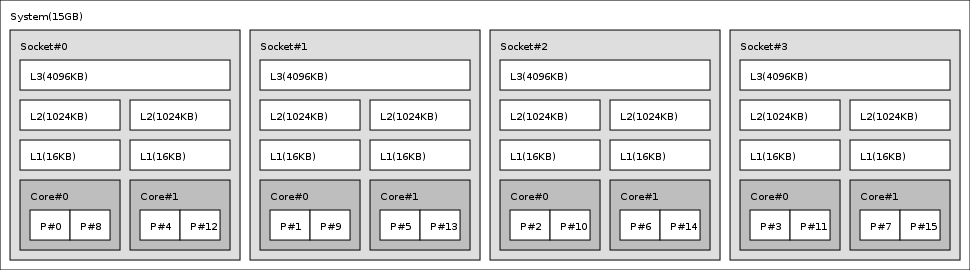
\includegraphics[width=\textwidth]{dudley.png}}
\end{DoxyImageNoCaption}


\begin{DoxyVerb}
System(15GB)
  Socket#0 + L3(4096KB)
    L2(1024KB) + L1(16KB) + Core#0
      P#0
      P#8
    L2(1024KB) + L1(16KB) + Core#1
      P#4
      P#12
  Socket#1 + L3(4096KB)
    L2(1024KB) + L1(16KB) + Core#0
      P#1
      P#9
    L2(1024KB) + L1(16KB) + Core#1
      P#5
      P#13
  Socket#2 + L3(4096KB)
    L2(1024KB) + L1(16KB) + Core#0
      P#2
      P#10
    L2(1024KB) + L1(16KB) + Core#1
      P#6
      P#14
  Socket#3 + L3(4096KB)
    L2(1024KB) + L1(16KB) + Core#0
      P#3
      P#11
    L2(1024KB) + L1(16KB) + Core#1
      P#7
      P#15
\end{DoxyVerb}


On a 4-\/socket 2-\/core Opteron NUMA machine, the {\ttfamily lstopo} tool may show the following outputs:

 
\begin{DoxyImageNoCaption}
  \mbox{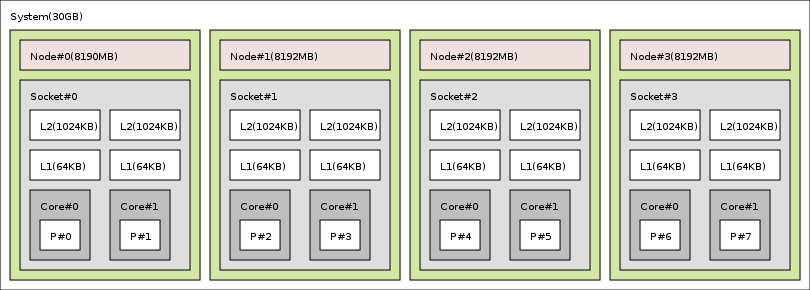
\includegraphics[width=\textwidth]{hagrid.png}}
\end{DoxyImageNoCaption}


\begin{DoxyVerb}
System(62GB)
  Node#0(8190MB) + Socket#0
    L2(1024KB) + L1(64KB) + Core#0 + P#0
    L2(1024KB) + L1(64KB) + Core#1 + P#1
  Node#1(8192MB) + Socket#1
    L2(1024KB) + L1(64KB) + Core#0 + P#2
    L2(1024KB) + L1(64KB) + Core#1 + P#3
  Node#2(8192MB) + Socket#2
    L2(1024KB) + L1(64KB) + Core#0 + P#4
    L2(1024KB) + L1(64KB) + Core#1 + P#5
  Node#3(8192MB) + Socket#3
    L2(1024KB) + L1(64KB) + Core#0 + P#6
    L2(1024KB) + L1(64KB) + Core#1 + P#7
  Node#4(8192MB) + Socket#4
    L2(1024KB) + L1(64KB) + Core#0 + P#8
    L2(1024KB) + L1(64KB) + Core#1 + P#9
  Node#5(8192MB) + Socket#5
    L2(1024KB) + L1(64KB) + Core#0 + P#10
    L2(1024KB) + L1(64KB) + Core#1 + P#11
  Node#6(8192MB) + Socket#6
    L2(1024KB) + L1(64KB) + Core#0 + P#12
    L2(1024KB) + L1(64KB) + Core#1 + P#13
  Node#7(8192MB) + Socket#7
    L2(1024KB) + L1(64KB) + Core#0 + P#14
    L2(1024KB) + L1(64KB) + Core#1 + P#15
\end{DoxyVerb}


On a 2-\/socket quad-\/core Xeon (pre-\/Nehalem, with 2 dual-\/core dies into each socket):

 
\begin{DoxyImageNoCaption}
  \mbox{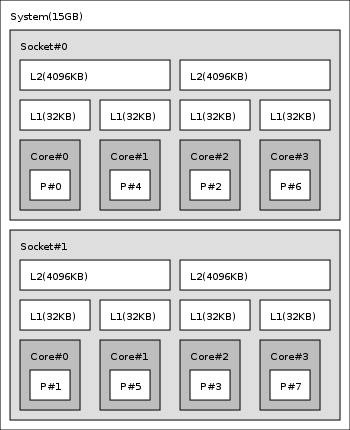
\includegraphics[width=8cm]{emmett.png}}
\end{DoxyImageNoCaption}


\begin{DoxyVerb}
System(15GB)
  Socket#0
    L2(4096KB)
      L1(32KB) + Core#0 + P#0
      L1(32KB) + Core#1 + P#4
    L2(4096KB)
      L1(32KB) + Core#2 + P#2
      L1(32KB) + Core#3 + P#6
  Socket#1
    L2(4096KB)
      L1(32KB) + Core#0 + P#1
      L1(32KB) + Core#1 + P#5
    L2(4096KB)
      L1(32KB) + Core#2 + P#3
      L1(32KB) + Core#3 + P#7
\end{DoxyVerb}


\hypertarget{index_interface}{}\section{Programming interface}\label{index_interface}
The basic interface is available in \hyperlink{hwloc_8h_source}{hwloc.h}. It mostly offers low-\/level routines for advanced programmers that want to manually manipulate objects and follow links between them. Developers should look at \hyperlink{helper_8h_source}{hwloc/helper.h}, which provides good higher-\/level topology traversal examples.

Each object contains a cpuset describing the list of processors that it contains. These cpusets may be used for \hyperlink{group__hwlocality__binding}{Binding}. hwloc offers an extensive cpuset manipulation interface in \hyperlink{cpuset_8h_source}{hwloc/cpuset.h}.

Moreover, hwloc also comes with additional helpers for interoperability with several commonly used environments. For Linux, some specific helpers are available in \hyperlink{linux_8h_source}{hwloc/linux.h}, and \hyperlink{linux-libnuma_8h_source}{hwloc/linux-\/libnuma.h} if using libnuma. On glibc-\/based systems, additional helpers are available in \hyperlink{glibc-sched_8h_source}{hwloc/glibc-\/sched.h}. For Linux systems with the OpenFabrics verbs library, some dedicated helpers are provided in \hyperlink{openfabrics-verbs_8h_source}{hwloc/openfabrics-\/verbs.h} (this helper file is not yet useful on non-\/Linux systems with the OpenFabrics verbs library).

To precisely define the vocabulary used by hwloc, a \hyperlink{index_glossary}{Glossary} is available and should probably be read first.

Further documentation is available in a full set of HTML pages, man pages, and self-\/contained PDF files (formatted for both both US letter and A4 formats) in the source tarball in doc/doxygen-\/doc/. If you are building from a Subversion checkout, you will need to have Doxygen and pdflatex installed -\/-\/ the documentation will be built during the normal \char`\"{}make\char`\"{} process. The documentation is installed during \char`\"{}make
install\char`\"{} to \$prefix/share/doc/hwloc/ and your systems default man page tree (under \$prefix, of course).

The following section presents an example of API usage.\hypertarget{index_interface_example}{}\section{API example}\label{index_interface_example}
The following small C example (named ``hwloc-\/hello.c'') prints the topology of the machine and bring the process to the first processor of the second core of the machine.


\begin{DoxyCodeInclude}
/* Example hwloc API program.
 *
 * Copyright © 2009 INRIA, Université Bordeaux 1
 * Copyright © 2009 Cisco Systems, Inc.  All rights reserved.
 *
 * hwloc-hello.c 
 */

#include <hwloc.h>

static void print_children(hwloc_topology_t topology, hwloc_obj_t obj, 
                           int depth)
{
    char string[128];
    int i;

    hwloc_obj_snprintf(string, sizeof(string), topology, obj, "#", 0);
    printf("%*s%s\n", 2*depth, "", string);
    for (i = 0; i < obj->arity; i++) {
        print_children(topology, obj->children[i], depth + 1);
    }
}

int main(int argc, char **argv)
{
    int depth, i;
    char string[128];
    unsigned int topodepth;
    hwloc_topology_t topology;
    hwloc_cpuset_t cpuset;
    hwloc_obj_t obj;

    /* Allocate and initialize topology object. */
    hwloc_topology_init(&topology);

    /* ... Optionally, put detection configuration here to e.g. ignore
       some objects types, define a synthetic topology, etc....  

       The default is to detect all the objects of the machine that
       the caller is allowed to access.  See Configure Topology
       Detection. */

    /* Perform the topology detection. */
    hwloc_topology_load(topology);

    /* Optionally, get some additional topology information
       in case we need the topology depth later. */
    topodepth = hwloc_topology_get_depth(topology);

    /* Walk the topology with an array style, from level 0 (always the
       system level) to the lowest level (always the proc level). */
    for (depth = 0; depth < topodepth; depth++) {
        printf("*** Objects at level %d\n", depth);
        for (i = 0; i < hwloc_get_nbobjs_by_depth(topology, depth); 
             i++) {
            hwloc_obj_snprintf(string, sizeof(string), topology,
                       hwloc_get_obj_by_depth(topology, depth, i),
                       "#", 0);
            printf("Index %d: %s\n", i, string);
        }
    }

    /* Walk the topology with a tree style. */
    printf("*** Printing overall tree\n");
    print_children(topology, hwloc_get_system_obj(topology), 0);

    /* Print the number of sockets. */
    depth = hwloc_get_type_depth(topology, HWLOC_OBJ_SOCKET);
    if (depth == HWLOC_TYPE_DEPTH_UNKNOWN) {
        printf("*** The number of sockets is unknown\n");
    } else {
        printf("*** %u socket(s)\n", 
               hwloc_get_nbobjs_by_depth(topology, depth));
    }

    /* Find out where cores are, or else smaller sets of CPUs if 
       the OS doesn't have the notion of a "core". */
    depth = hwloc_get_type_or_below_depth(topology, HWLOC_OBJ_CORE);

    /* Get last level. */
    obj = hwloc_get_obj_by_depth(topology, depth, 
                   hwloc_get_nbobjs_by_depth(topology, depth) - 1);
    if (obj) {
        /* Get a copy of its cpuset that we may modify. */
        cpuset = hwloc_cpuset_dup(obj->cpuset);
    
        /* Get only one logical processor (in case the core is
           SMT/hyperthreaded). */
        hwloc_cpuset_singlify(cpuset);

        /* And try to bind ourself there. */
        if (hwloc_set_cpubind(topology, cpuset, 0)) {
            char *str;
            hwloc_cpuset_asprintf(&str, obj->cpuset);
            printf("Couldn't bind to cpuset %s\n", str);
            free(str);
        }

        /* Free our cpuset copy */
        hwloc_cpuset_free(cpuset);
    }

    /* Destroy topology object. */
    hwloc_topology_destroy(topology);

    return 0;
}
\end{DoxyCodeInclude}


hwloc provides a {\ttfamily pkg-\/config} executable to obtain relevant compiler and linker flags. For example, it can be used thusly to compile applications that utilize the hwloc library (assuming GNU Make):

\begin{DoxyVerb}
CFLAGS += $(pkg-config --cflags hwloc)
LDLIBS += $(pkg-config --libs hwloc)
cc hwloc-hello.c $(CFLAGS) -o hwloc-hello $(LDLIBS)
\end{DoxyVerb}


On a machine with 4GB of RAM and 2 processor sockets -\/-\/ each socket of which has two processor cores -\/-\/ the output from running {\ttfamily hwloc-\/hello} could be something like the following:

\begin{DoxyVerb}
shell$ ./hwloc-hello
*** Objects at level 0
Index 0: System(3938MB)
*** Objects at level 1
Index 0: Socket#0
Index 1: Socket#1
*** Objects at level 2
Index 0: Core#0
Index 1: Core#1
Index 2: Core#3
Index 3: Core#2
*** Objects at level 3
Index 0: P#0
Index 1: P#1
Index 2: P#2
Index 3: P#3
*** Printing overall tree
System(3938MB)
  Socket#0
    Core#0
      P#0
    Core#1
      P#1
  Socket#1
    Core#3
      P#2
    Core#2
      P#3
*** 2 socket(s)
shell$ 
\end{DoxyVerb}


 \hypertarget{index_bugs}{}\section{Questions and bugs}\label{index_bugs}
Questions should be sent to the devel mailing list (\href{http://www.open-mpi.org/community/lists/hwloc.php}{\tt http://www.open-\/mpi.org/community/lists/hwloc.php}). Bug reports should be reported in the tracker (\href{https://svn.open-mpi.org/trac/hwloc/}{\tt https://svn.open-\/mpi.org/trac/hwloc/}).

 \hypertarget{index_history}{}\section{History / credits}\label{index_history}
hwloc is the evolution and merger of the libtopology (\href{http://runtime.bordeaux.inria.fr/libtopology/}{\tt http://runtime.bordeaux.inria.fr/libtopology/}) project and the Portable Linux Processor Affinity (PLPA) (\href{http://www.open-mpi.org/projects/plpa/}{\tt http://www.open-\/mpi.org/projects/plpa/}) project. Because of functional and ideological overlap, these two code bases and ideas were merged and released under the name \char`\"{}hwloc\char`\"{} as an Open MPI sub-\/project.

libtopology was initially developed by the INRIA Runtime Team-\/Project (\href{http://runtime.bordeaux.inria.fr/}{\tt http://runtime.bordeaux.inria.fr/}) (headed by Raymond Namyst (\href{http://dept-info.labri.fr/~namyst/}{\tt http://dept-\/info.labri.fr/$\sim$namyst/}). PLPA was initially developed by the Open MPI development team as a sub-\/project. Both are now deprecated in favor of hwloc, which is distributed as an Open MPI sub-\/project.

\hypertarget{index_glossary}{}\section{Glossary}\label{index_glossary}

\begin{DoxyDescription}
\item[Object ]Interesting kind of part of the system, such as a Core, a Cache, a Memory node, etc. The different types detected by hwloc are detailed in the \hyperlink{group__hwlocality__types_gacd37bb612667dc437d66bfb175a8dc55}{hwloc\_\-obj\_\-type\_\-t} enumeration.

They are topologically sorted by CPU set into a tree whose root is the System object (which always exists). 


\item[CPU set ]The set of logical processors logically included in an object (if any). This term does {\itshape not\/} have any relation to an operating system ``CPU set.''


\item[Father object ]The object logically containing the current object, for example because its CPU set includes the CPU set of the current object.


\item[Children object(s) ]The object (or objects) contained in the current object because their CPU set is included in the CPU set of the current object.


\item[Arity ]The number of children of an object.


\item[Sibling objects ]Objects of the same type which have the same father.


\item[Sibling rank ]Index to uniquely identify objects of the same type which have the same father, and is always in the range \mbox{[}0, fathers\_\-arity).


\item[Cousin objects ]Objects of the same type as the current object.


\item[Level ]Set of objects of the same type.


\item[OS index ]The index that the operating system (OS) uses to identify the object. This may be completely arbitrary, or it may depend on the BIOS configuration.


\item[Depth ]Nesting level in the object tree, starting from the 0th object (i.e., the System object).


\item[Logical index ]Index to uniquely identify objects of the same type. It is generally used to express proximity. This index is always linear and in the range \mbox{[}0, num\_\-objs\_\-same\_\-type\_\-same\_\-level). Think of it as ``cousin rank.''


\end{DoxyDescription}

The following diagram can help to understand the vocabulary of the relationships by showing the example of a machine with two dual core sockets (with no hardware threads); thus, a topology with 4 levels.

 
\begin{DoxyImageNoCaption}
  \mbox{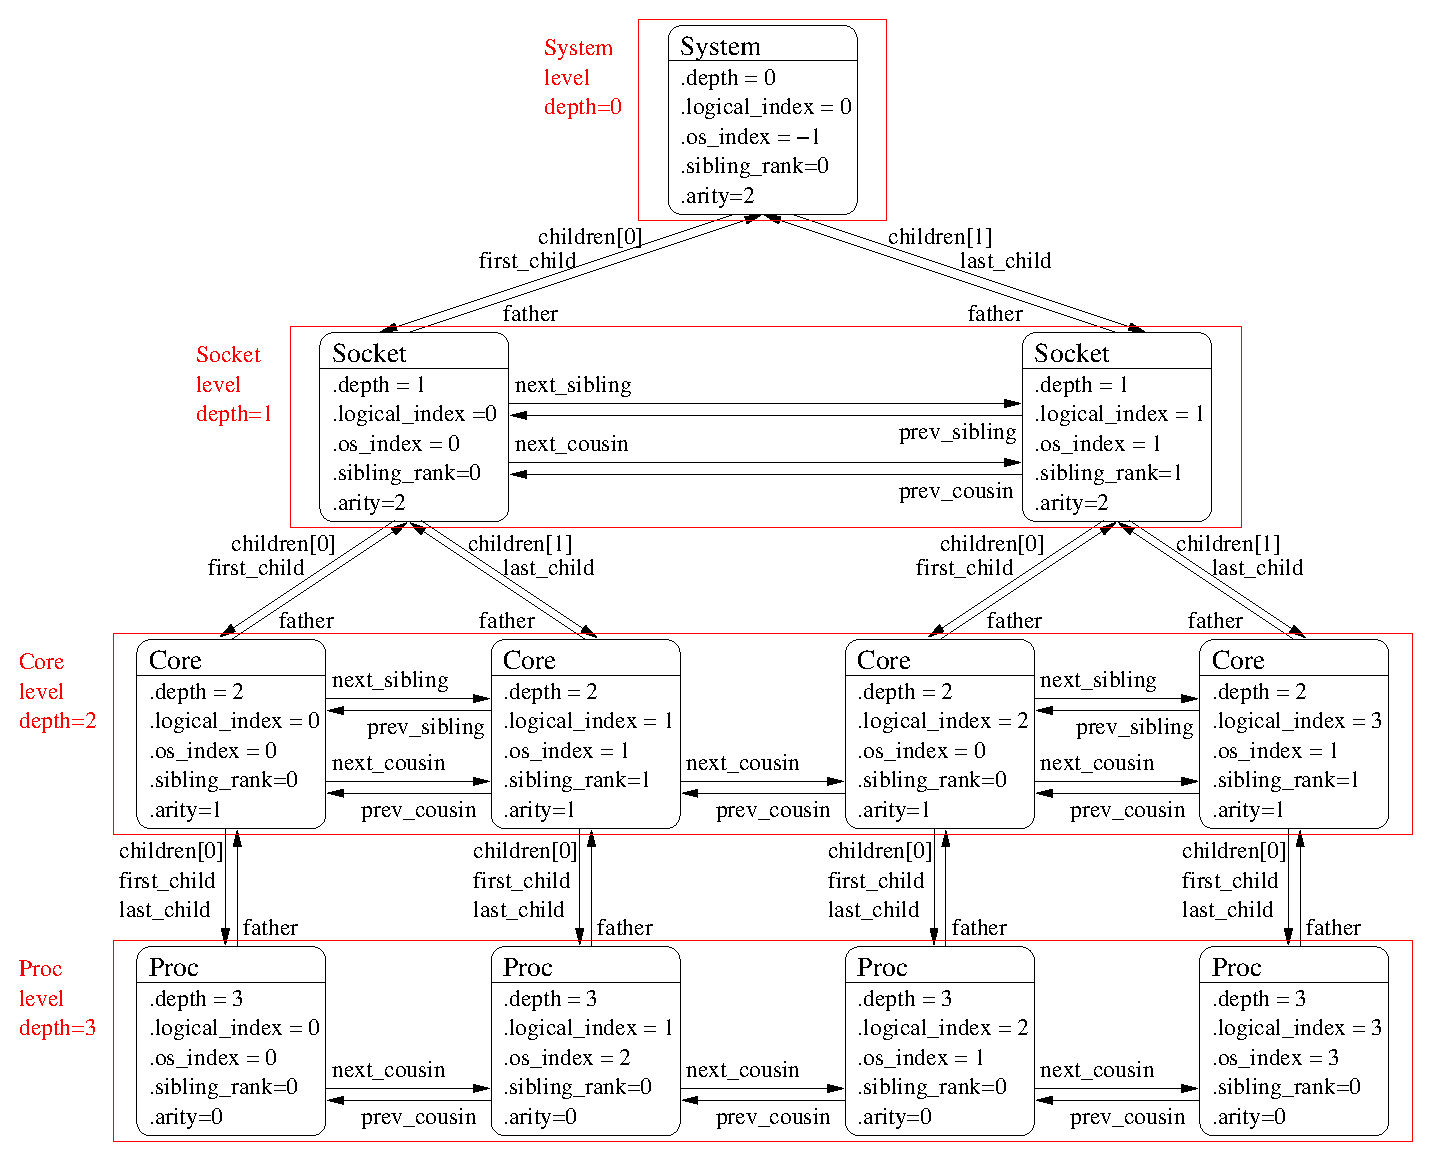
\includegraphics[width=\textwidth]{diagram}}
\end{DoxyImageNoCaption}


It should be noted that for Processor objects, the logical index -\/-\/ as computed linearly by hwloc -\/-\/ is not the same as the OS index. 

\chapter{Module Index}
\section{Modules}
Here is a list of all modules:\begin{DoxyCompactList}
\item \contentsline{section}{Topology context}{\pageref{group__hwlocality__topology}}{}
\item \contentsline{section}{Topology Object Types}{\pageref{group__hwlocality__types}}{}
\item \contentsline{section}{Topology Objects}{\pageref{group__hwlocality__objects}}{}
\item \contentsline{section}{Create and Destroy Topologies}{\pageref{group__hwlocality__creation}}{}
\item \contentsline{section}{Configure Topology Detection}{\pageref{group__hwlocality__configuration}}{}
\item \contentsline{section}{Get some Topology Information}{\pageref{group__hwlocality__information}}{}
\item \contentsline{section}{Retrieve Objects}{\pageref{group__hwlocality__traversal}}{}
\item \contentsline{section}{Object/String Conversion}{\pageref{group__hwlocality__conversion}}{}
\item \contentsline{section}{Binding}{\pageref{group__hwlocality__binding}}{}
\item \contentsline{section}{Object Type Helpers}{\pageref{group__hwlocality__helper__types}}{}
\item \contentsline{section}{Basic Traversal Helpers}{\pageref{group__hwlocality__helper__traversal__basic}}{}
\item \contentsline{section}{Finding Objects Inside a CPU set}{\pageref{group__hwlocality__helper__find__inside}}{}
\item \contentsline{section}{Finding a single Object covering at least CPU set}{\pageref{group__hwlocality__helper__find__covering}}{}
\item \contentsline{section}{Finding a set of similar Objects covering at least a CPU set}{\pageref{group__hwlocality__helper__find__coverings}}{}
\item \contentsline{section}{Cache-\/specific Finding Helpers}{\pageref{group__hwlocality__helper__find__cache}}{}
\item \contentsline{section}{Advanced Traversal Helpers}{\pageref{group__hwlocality__helper__traversal}}{}
\item \contentsline{section}{Binding Helpers}{\pageref{group__hwlocality__helper__binding}}{}
\item \contentsline{section}{The Cpuset API}{\pageref{group__hwlocality__cpuset}}{}
\item \contentsline{section}{Helpers for manipulating glibc sched affinity}{\pageref{group__hwlocality__glibc__sched}}{}
\item \contentsline{section}{Helpers for manipulating linux kernel cpumap files}{\pageref{group__hwlocality__linux__cpumap}}{}
\item \contentsline{section}{Helpers for manipulating Linux libnuma unsigned long masks}{\pageref{group__hwlocality__linux__libnuma__ulongs}}{}
\item \contentsline{section}{Helpers for manipulating Linux libnuma bitmask}{\pageref{group__hwlocality__linux__libnuma__bitmask}}{}
\item \contentsline{section}{Helpers for manipulating Linux libnuma nodemask\_\-t}{\pageref{group__hwlocality__linux__libnuma__nodemask}}{}
\item \contentsline{section}{OpenFabrics-\/Specific Functions}{\pageref{group__hwloc__openfabrics}}{}
\end{DoxyCompactList}

\chapter{Data Structure Index}
\section{Data Structures}
Here are the data structures with brief descriptions:\begin{DoxyCompactList}
\item\contentsline{section}{\hyperlink{structhwloc__obj__attr__u_1_1hwloc__cache__attr__s}{hwloc\_\-obj\_\-attr\_\-u::hwloc\_\-cache\_\-attr\_\-s} (Cache-\/specific Object Attributes )}{\pageref{structhwloc__obj__attr__u_1_1hwloc__cache__attr__s}}{}
\item\contentsline{section}{\hyperlink{structhwloc__obj__attr__u_1_1hwloc__machine__attr__s}{hwloc\_\-obj\_\-attr\_\-u::hwloc\_\-machine\_\-attr\_\-s} (Machine-\/specific Object Attributes )}{\pageref{structhwloc__obj__attr__u_1_1hwloc__machine__attr__s}}{}
\item\contentsline{section}{\hyperlink{structhwloc__obj__attr__u_1_1hwloc__memory__attr__s}{hwloc\_\-obj\_\-attr\_\-u::hwloc\_\-memory\_\-attr\_\-s} (Node-\/specific Object Attributes )}{\pageref{structhwloc__obj__attr__u_1_1hwloc__memory__attr__s}}{}
\item\contentsline{section}{\hyperlink{structhwloc__obj__attr__u_1_1hwloc__misc__attr__s}{hwloc\_\-obj\_\-attr\_\-u::hwloc\_\-misc\_\-attr\_\-s} (Misc-\/specific Object Attributes )}{\pageref{structhwloc__obj__attr__u_1_1hwloc__misc__attr__s}}{}
\item\contentsline{section}{\hyperlink{structhwloc__obj}{hwloc\_\-obj} (Structure of a topology object )}{\pageref{structhwloc__obj}}{}
\item\contentsline{section}{\hyperlink{unionhwloc__obj__attr__u}{hwloc\_\-obj\_\-attr\_\-u} (Object type-\/specific Attributes )}{\pageref{unionhwloc__obj__attr__u}}{}
\end{DoxyCompactList}

\chapter{Module Documentation}
\hypertarget{group__hwlocality__topology}{
\section{Topology context}
\label{group__hwlocality__topology}\index{Topology context@{Topology context}}
}
\subsection*{Typedefs}
\begin{DoxyCompactItemize}
\item 
typedef struct hwloc\_\-topology $\ast$ \hyperlink{group__hwlocality__topology_ga9d1e76ee15a7dee158b786c30b6a6e38}{hwloc\_\-topology\_\-t}
\begin{DoxyCompactList}\small\item\em Topology context. \item\end{DoxyCompactList}\end{DoxyCompactItemize}


\subsection{Typedef Documentation}
\hypertarget{group__hwlocality__topology_ga9d1e76ee15a7dee158b786c30b6a6e38}{
\index{hwlocality\_\-topology@{hwlocality\_\-topology}!hwloc\_\-topology\_\-t@{hwloc\_\-topology\_\-t}}
\index{hwloc\_\-topology\_\-t@{hwloc\_\-topology\_\-t}!hwlocality_topology@{hwlocality\_\-topology}}
\subsubsection[{hwloc\_\-topology\_\-t}]{\setlength{\rightskip}{0pt plus 5cm}typedef struct hwloc\_\-topology$\ast$ {\bf hwloc\_\-topology\_\-t}}}
\label{group__hwlocality__topology_ga9d1e76ee15a7dee158b786c30b6a6e38}


Topology context. To be initialized with \hyperlink{group__hwlocality__creation_ga03fd4a16d8b9ee1ffc32b25fd2f6bdfa}{hwloc\_\-topology\_\-init()} and built with \hyperlink{group__hwlocality__creation_gabdf58d87ad77f6615fccdfe0535ff826}{hwloc\_\-topology\_\-load()}. 

\hypertarget{group__hwlocality__types}{
\section{Topology Object Types}
\label{group__hwlocality__types}\index{Topology Object Types@{Topology Object Types}}
}
\subsection*{Defines}
\begin{DoxyCompactItemize}
\item 
\#define \hyperlink{group__hwlocality__types_ga3b6e4128e9fe773863b123fa6e4a080b}{HWLOC\_\-TYPE\_\-UNORDERED}~INT\_\-MAX
\begin{DoxyCompactList}\small\item\em Value returned by hwloc\_\-compare\_\-types when types can not be compared. \item\end{DoxyCompactList}\end{DoxyCompactItemize}
\subsection*{Enumerations}
\begin{DoxyCompactItemize}
\item 
enum \hyperlink{group__hwlocality__types_gacd37bb612667dc437d66bfb175a8dc55}{hwloc\_\-obj\_\-type\_\-t} \{ \par
\hyperlink{group__hwlocality__types_ggacd37bb612667dc437d66bfb175a8dc55a3aa1b842d1fd4207ebce171f95a244ec}{HWLOC\_\-OBJ\_\-SYSTEM}, 
\hyperlink{group__hwlocality__types_ggacd37bb612667dc437d66bfb175a8dc55a3f4e83ffc4a259354959ae8a9eaa2a80}{HWLOC\_\-OBJ\_\-MACHINE}, 
\hyperlink{group__hwlocality__types_ggacd37bb612667dc437d66bfb175a8dc55aaf0964881117bdedf1a5e9332cd120dd}{HWLOC\_\-OBJ\_\-NODE}, 
\hyperlink{group__hwlocality__types_ggacd37bb612667dc437d66bfb175a8dc55a1ac6e07775ae4324b3fe9dbd72c785ec}{HWLOC\_\-OBJ\_\-SOCKET}, 
\par
\hyperlink{group__hwlocality__types_ggacd37bb612667dc437d66bfb175a8dc55a56ee0b7eca88f363b75b34fdde8c9ddc}{HWLOC\_\-OBJ\_\-CACHE}, 
\hyperlink{group__hwlocality__types_ggacd37bb612667dc437d66bfb175a8dc55ac793958f330bca371aa1535de8aff45f}{HWLOC\_\-OBJ\_\-CORE}, 
\hyperlink{group__hwlocality__types_ggacd37bb612667dc437d66bfb175a8dc55a5e0ccbbd5922cbb07b53fe892b91b8f2}{HWLOC\_\-OBJ\_\-PROC}, 
\hyperlink{group__hwlocality__types_ggacd37bb612667dc437d66bfb175a8dc55a19f8a6953fa91efc76bcbcdf2d22de4d}{HWLOC\_\-OBJ\_\-MISC}
 \}
\begin{DoxyCompactList}\small\item\em Type of topology object. \item\end{DoxyCompactList}\end{DoxyCompactItemize}
\subsection*{Functions}
\begin{DoxyCompactItemize}
\item 
int \hyperlink{group__hwlocality__types_ga1820ea0dfd8e9dca28f9ea7624df5ae2}{hwloc\_\-compare\_\-types} (\hyperlink{group__hwlocality__types_gacd37bb612667dc437d66bfb175a8dc55}{hwloc\_\-obj\_\-type\_\-t} type1, \hyperlink{group__hwlocality__types_gacd37bb612667dc437d66bfb175a8dc55}{hwloc\_\-obj\_\-type\_\-t} type2)
\begin{DoxyCompactList}\small\item\em Compare the depth of two object types. \item\end{DoxyCompactList}\end{DoxyCompactItemize}


\subsection{Define Documentation}
\hypertarget{group__hwlocality__types_ga3b6e4128e9fe773863b123fa6e4a080b}{
\index{hwlocality\_\-types@{hwlocality\_\-types}!HWLOC\_\-TYPE\_\-UNORDERED@{HWLOC\_\-TYPE\_\-UNORDERED}}
\index{HWLOC\_\-TYPE\_\-UNORDERED@{HWLOC\_\-TYPE\_\-UNORDERED}!hwlocality_types@{hwlocality\_\-types}}
\subsubsection[{HWLOC\_\-TYPE\_\-UNORDERED}]{\setlength{\rightskip}{0pt plus 5cm}\#define HWLOC\_\-TYPE\_\-UNORDERED~INT\_\-MAX}}
\label{group__hwlocality__types_ga3b6e4128e9fe773863b123fa6e4a080b}


Value returned by hwloc\_\-compare\_\-types when types can not be compared. 

\subsection{Enumeration Type Documentation}
\hypertarget{group__hwlocality__types_gacd37bb612667dc437d66bfb175a8dc55}{
\index{hwlocality\_\-types@{hwlocality\_\-types}!hwloc\_\-obj\_\-type\_\-t@{hwloc\_\-obj\_\-type\_\-t}}
\index{hwloc\_\-obj\_\-type\_\-t@{hwloc\_\-obj\_\-type\_\-t}!hwlocality_types@{hwlocality\_\-types}}
\subsubsection[{hwloc\_\-obj\_\-type\_\-t}]{\setlength{\rightskip}{0pt plus 5cm}enum {\bf hwloc\_\-obj\_\-type\_\-t}}}
\label{group__hwlocality__types_gacd37bb612667dc437d66bfb175a8dc55}


Type of topology object. \begin{DoxyNote}{Note}
Do not rely on the ordering or completeness of the values as new ones may be defined in the future! If you need to compare types, use \hyperlink{group__hwlocality__types_ga1820ea0dfd8e9dca28f9ea7624df5ae2}{hwloc\_\-compare\_\-types()} instead. 
\end{DoxyNote}
\begin{Desc}
\item[Enumerator: ]\par
\begin{description}
\index{HWLOC\_\-OBJ\_\-SYSTEM@{HWLOC\_\-OBJ\_\-SYSTEM}!hwlocality\_\-types@{hwlocality\_\-types}}\index{hwlocality\_\-types@{hwlocality\_\-types}!HWLOC\_\-OBJ\_\-SYSTEM@{HWLOC\_\-OBJ\_\-SYSTEM}}\item[{\em 
\hypertarget{group__hwlocality__types_ggacd37bb612667dc437d66bfb175a8dc55a3aa1b842d1fd4207ebce171f95a244ec}{
HWLOC\_\-OBJ\_\-SYSTEM}
\label{group__hwlocality__types_ggacd37bb612667dc437d66bfb175a8dc55a3aa1b842d1fd4207ebce171f95a244ec}
}]Whole system (may be a cluster of machines). The whole system that is accessible to hwloc. That may comprise several machines in SSI systems like Kerrighed. \index{HWLOC\_\-OBJ\_\-MACHINE@{HWLOC\_\-OBJ\_\-MACHINE}!hwlocality\_\-types@{hwlocality\_\-types}}\index{hwlocality\_\-types@{hwlocality\_\-types}!HWLOC\_\-OBJ\_\-MACHINE@{HWLOC\_\-OBJ\_\-MACHINE}}\item[{\em 
\hypertarget{group__hwlocality__types_ggacd37bb612667dc437d66bfb175a8dc55a3f4e83ffc4a259354959ae8a9eaa2a80}{
HWLOC\_\-OBJ\_\-MACHINE}
\label{group__hwlocality__types_ggacd37bb612667dc437d66bfb175a8dc55a3f4e83ffc4a259354959ae8a9eaa2a80}
}]Machine. A set of processors and memory with cache coherency. \index{HWLOC\_\-OBJ\_\-NODE@{HWLOC\_\-OBJ\_\-NODE}!hwlocality\_\-types@{hwlocality\_\-types}}\index{hwlocality\_\-types@{hwlocality\_\-types}!HWLOC\_\-OBJ\_\-NODE@{HWLOC\_\-OBJ\_\-NODE}}\item[{\em 
\hypertarget{group__hwlocality__types_ggacd37bb612667dc437d66bfb175a8dc55aaf0964881117bdedf1a5e9332cd120dd}{
HWLOC\_\-OBJ\_\-NODE}
\label{group__hwlocality__types_ggacd37bb612667dc437d66bfb175a8dc55aaf0964881117bdedf1a5e9332cd120dd}
}]NUMA node. A set of processors around memory which the processors can directly access. \index{HWLOC\_\-OBJ\_\-SOCKET@{HWLOC\_\-OBJ\_\-SOCKET}!hwlocality\_\-types@{hwlocality\_\-types}}\index{hwlocality\_\-types@{hwlocality\_\-types}!HWLOC\_\-OBJ\_\-SOCKET@{HWLOC\_\-OBJ\_\-SOCKET}}\item[{\em 
\hypertarget{group__hwlocality__types_ggacd37bb612667dc437d66bfb175a8dc55a1ac6e07775ae4324b3fe9dbd72c785ec}{
HWLOC\_\-OBJ\_\-SOCKET}
\label{group__hwlocality__types_ggacd37bb612667dc437d66bfb175a8dc55a1ac6e07775ae4324b3fe9dbd72c785ec}
}]Socket, physical package, or chip. In the physical meaning, i.e. that you can add or remove physically. \index{HWLOC\_\-OBJ\_\-CACHE@{HWLOC\_\-OBJ\_\-CACHE}!hwlocality\_\-types@{hwlocality\_\-types}}\index{hwlocality\_\-types@{hwlocality\_\-types}!HWLOC\_\-OBJ\_\-CACHE@{HWLOC\_\-OBJ\_\-CACHE}}\item[{\em 
\hypertarget{group__hwlocality__types_ggacd37bb612667dc437d66bfb175a8dc55a56ee0b7eca88f363b75b34fdde8c9ddc}{
HWLOC\_\-OBJ\_\-CACHE}
\label{group__hwlocality__types_ggacd37bb612667dc437d66bfb175a8dc55a56ee0b7eca88f363b75b34fdde8c9ddc}
}]Data cache. Can be L1, L2, L3, ... \index{HWLOC\_\-OBJ\_\-CORE@{HWLOC\_\-OBJ\_\-CORE}!hwlocality\_\-types@{hwlocality\_\-types}}\index{hwlocality\_\-types@{hwlocality\_\-types}!HWLOC\_\-OBJ\_\-CORE@{HWLOC\_\-OBJ\_\-CORE}}\item[{\em 
\hypertarget{group__hwlocality__types_ggacd37bb612667dc437d66bfb175a8dc55ac793958f330bca371aa1535de8aff45f}{
HWLOC\_\-OBJ\_\-CORE}
\label{group__hwlocality__types_ggacd37bb612667dc437d66bfb175a8dc55ac793958f330bca371aa1535de8aff45f}
}]Core. A computation unit (may be shared by several logical processors). \index{HWLOC\_\-OBJ\_\-PROC@{HWLOC\_\-OBJ\_\-PROC}!hwlocality\_\-types@{hwlocality\_\-types}}\index{hwlocality\_\-types@{hwlocality\_\-types}!HWLOC\_\-OBJ\_\-PROC@{HWLOC\_\-OBJ\_\-PROC}}\item[{\em 
\hypertarget{group__hwlocality__types_ggacd37bb612667dc437d66bfb175a8dc55a5e0ccbbd5922cbb07b53fe892b91b8f2}{
HWLOC\_\-OBJ\_\-PROC}
\label{group__hwlocality__types_ggacd37bb612667dc437d66bfb175a8dc55a5e0ccbbd5922cbb07b53fe892b91b8f2}
}](Logical) Processor. An execution unit (may share a core with some other logical processors, e.g. in the case of an SMT core). Objects of this kind are always reported and can thus be used as fallback when others are not. \index{HWLOC\_\-OBJ\_\-MISC@{HWLOC\_\-OBJ\_\-MISC}!hwlocality\_\-types@{hwlocality\_\-types}}\index{hwlocality\_\-types@{hwlocality\_\-types}!HWLOC\_\-OBJ\_\-MISC@{HWLOC\_\-OBJ\_\-MISC}}\item[{\em 
\hypertarget{group__hwlocality__types_ggacd37bb612667dc437d66bfb175a8dc55a19f8a6953fa91efc76bcbcdf2d22de4d}{
HWLOC\_\-OBJ\_\-MISC}
\label{group__hwlocality__types_ggacd37bb612667dc437d66bfb175a8dc55a19f8a6953fa91efc76bcbcdf2d22de4d}
}]Miscellaneous objects. Objects which do not fit in the above but are detected by hwloc and are useful to take into account for affinity. For instance, some OSes expose their arbitrary processors aggregation this way. \end{description}
\end{Desc}



\subsection{Function Documentation}
\hypertarget{group__hwlocality__types_ga1820ea0dfd8e9dca28f9ea7624df5ae2}{
\index{hwlocality\_\-types@{hwlocality\_\-types}!hwloc\_\-compare\_\-types@{hwloc\_\-compare\_\-types}}
\index{hwloc\_\-compare\_\-types@{hwloc\_\-compare\_\-types}!hwlocality_types@{hwlocality\_\-types}}
\subsubsection[{hwloc\_\-compare\_\-types}]{\setlength{\rightskip}{0pt plus 5cm}int hwloc\_\-compare\_\-types ({\bf hwloc\_\-obj\_\-type\_\-t} {\em type1}, \/  {\bf hwloc\_\-obj\_\-type\_\-t} {\em type2})}}
\label{group__hwlocality__types_ga1820ea0dfd8e9dca28f9ea7624df5ae2}


Compare the depth of two object types. Types shouldn't be compared as they are, since newer ones may be added in the future. This function returns less than, equal to, or greater than zero if {\ttfamily type1} is considered to be respectively higher than, equal to, or deeper than {\ttfamily type2} in the hierarchy. If the types can not be compared (because it does not make sense), HWLOC\_\-TYPE\_\-UNORDERED is returned. Object types containing CPUs can always be compared.

\begin{DoxyNote}{Note}
HWLOC\_\-OBJ\_\-SYSTEM will always be the highest, and HWLOC\_\-OBJ\_\-PROC will always be the deepest. 
\end{DoxyNote}

\hypertarget{group__hwlocality__objects}{
\section{Topology Objects}
\label{group__hwlocality__objects}\index{Topology Objects@{Topology Objects}}
}
\subsection*{Data Structures}
\begin{DoxyCompactItemize}
\item 
struct \hyperlink{structhwloc__obj}{hwloc\_\-obj}
\begin{DoxyCompactList}\small\item\em Structure of a topology object. \item\end{DoxyCompactList}\item 
union \hyperlink{unionhwloc__obj__attr__u}{hwloc\_\-obj\_\-attr\_\-u}
\begin{DoxyCompactList}\small\item\em Object type-\/specific Attributes. \item\end{DoxyCompactList}\end{DoxyCompactItemize}
\subsection*{Typedefs}
\begin{DoxyCompactItemize}
\item 
typedef struct \hyperlink{structhwloc__obj}{hwloc\_\-obj} $\ast$ \hyperlink{group__hwlocality__objects_ga79b8ab56877ef99ac59b833203391c7d}{hwloc\_\-obj\_\-t}
\end{DoxyCompactItemize}


\subsection{Typedef Documentation}
\hypertarget{group__hwlocality__objects_ga79b8ab56877ef99ac59b833203391c7d}{
\index{hwlocality\_\-objects@{hwlocality\_\-objects}!hwloc\_\-obj\_\-t@{hwloc\_\-obj\_\-t}}
\index{hwloc\_\-obj\_\-t@{hwloc\_\-obj\_\-t}!hwlocality_objects@{hwlocality\_\-objects}}
\subsubsection[{hwloc\_\-obj\_\-t}]{\setlength{\rightskip}{0pt plus 5cm}typedef struct {\bf hwloc\_\-obj}$\ast$ {\bf hwloc\_\-obj\_\-t}}}
\label{group__hwlocality__objects_ga79b8ab56877ef99ac59b833203391c7d}

\hypertarget{group__hwlocality__creation}{
\section{Create and Destroy Topologies}
\label{group__hwlocality__creation}\index{Create and Destroy Topologies@{Create and Destroy Topologies}}
}
\subsection*{Functions}
\begin{DoxyCompactItemize}
\item 
int \hyperlink{group__hwlocality__creation_ga03fd4a16d8b9ee1ffc32b25fd2f6bdfa}{hwloc\_\-topology\_\-init} (\hyperlink{group__hwlocality__topology_ga9d1e76ee15a7dee158b786c30b6a6e38}{hwloc\_\-topology\_\-t} $\ast$topologyp)
\begin{DoxyCompactList}\small\item\em Allocate a topology context. \item\end{DoxyCompactList}\item 
int \hyperlink{group__hwlocality__creation_gabdf58d87ad77f6615fccdfe0535ff826}{hwloc\_\-topology\_\-load} (\hyperlink{group__hwlocality__topology_ga9d1e76ee15a7dee158b786c30b6a6e38}{hwloc\_\-topology\_\-t} topology)
\begin{DoxyCompactList}\small\item\em Build the actual topology. \item\end{DoxyCompactList}\item 
void \hyperlink{group__hwlocality__creation_ga9f34a640b6fd28d23699d4d084667b15}{hwloc\_\-topology\_\-destroy} (\hyperlink{group__hwlocality__topology_ga9d1e76ee15a7dee158b786c30b6a6e38}{hwloc\_\-topology\_\-t} topology)
\begin{DoxyCompactList}\small\item\em Terminate and free a topology context. \item\end{DoxyCompactList}\item 
void \hyperlink{group__hwlocality__creation_gaf6746bc3a558ef1ac8348b4491d091b5}{hwloc\_\-topology\_\-check} (\hyperlink{group__hwlocality__topology_ga9d1e76ee15a7dee158b786c30b6a6e38}{hwloc\_\-topology\_\-t} topology)
\begin{DoxyCompactList}\small\item\em Run internal checks on a topology structure. \item\end{DoxyCompactList}\end{DoxyCompactItemize}


\subsection{Function Documentation}
\hypertarget{group__hwlocality__creation_gaf6746bc3a558ef1ac8348b4491d091b5}{
\index{hwlocality\_\-creation@{hwlocality\_\-creation}!hwloc\_\-topology\_\-check@{hwloc\_\-topology\_\-check}}
\index{hwloc\_\-topology\_\-check@{hwloc\_\-topology\_\-check}!hwlocality_creation@{hwlocality\_\-creation}}
\subsubsection[{hwloc\_\-topology\_\-check}]{\setlength{\rightskip}{0pt plus 5cm}void hwloc\_\-topology\_\-check ({\bf hwloc\_\-topology\_\-t} {\em topology})}}
\label{group__hwlocality__creation_gaf6746bc3a558ef1ac8348b4491d091b5}


Run internal checks on a topology structure. 
\begin{DoxyParams}{Parameters}
\item[{\em topology}]is the topology to be checked \end{DoxyParams}
\hypertarget{group__hwlocality__creation_ga9f34a640b6fd28d23699d4d084667b15}{
\index{hwlocality\_\-creation@{hwlocality\_\-creation}!hwloc\_\-topology\_\-destroy@{hwloc\_\-topology\_\-destroy}}
\index{hwloc\_\-topology\_\-destroy@{hwloc\_\-topology\_\-destroy}!hwlocality_creation@{hwlocality\_\-creation}}
\subsubsection[{hwloc\_\-topology\_\-destroy}]{\setlength{\rightskip}{0pt plus 5cm}void hwloc\_\-topology\_\-destroy ({\bf hwloc\_\-topology\_\-t} {\em topology})}}
\label{group__hwlocality__creation_ga9f34a640b6fd28d23699d4d084667b15}


Terminate and free a topology context. 
\begin{DoxyParams}{Parameters}
\item[{\em topology}]is the topology to be freed \end{DoxyParams}
\hypertarget{group__hwlocality__creation_ga03fd4a16d8b9ee1ffc32b25fd2f6bdfa}{
\index{hwlocality\_\-creation@{hwlocality\_\-creation}!hwloc\_\-topology\_\-init@{hwloc\_\-topology\_\-init}}
\index{hwloc\_\-topology\_\-init@{hwloc\_\-topology\_\-init}!hwlocality_creation@{hwlocality\_\-creation}}
\subsubsection[{hwloc\_\-topology\_\-init}]{\setlength{\rightskip}{0pt plus 5cm}int hwloc\_\-topology\_\-init ({\bf hwloc\_\-topology\_\-t} $\ast$ {\em topologyp})}}
\label{group__hwlocality__creation_ga03fd4a16d8b9ee1ffc32b25fd2f6bdfa}


Allocate a topology context. 
\begin{DoxyParams}{Parameters}
\item[\mbox{$\rightarrow$} {\em topologyp}]is assigned a pointer to the new allocated context.\end{DoxyParams}
\begin{DoxyReturn}{Returns}
0 on success, -\/1 on error. 
\end{DoxyReturn}
\hypertarget{group__hwlocality__creation_gabdf58d87ad77f6615fccdfe0535ff826}{
\index{hwlocality\_\-creation@{hwlocality\_\-creation}!hwloc\_\-topology\_\-load@{hwloc\_\-topology\_\-load}}
\index{hwloc\_\-topology\_\-load@{hwloc\_\-topology\_\-load}!hwlocality_creation@{hwlocality\_\-creation}}
\subsubsection[{hwloc\_\-topology\_\-load}]{\setlength{\rightskip}{0pt plus 5cm}int hwloc\_\-topology\_\-load ({\bf hwloc\_\-topology\_\-t} {\em topology})}}
\label{group__hwlocality__creation_gabdf58d87ad77f6615fccdfe0535ff826}


Build the actual topology. Build the actual topology once initialized with \hyperlink{group__hwlocality__creation_ga03fd4a16d8b9ee1ffc32b25fd2f6bdfa}{hwloc\_\-topology\_\-init()} and tuned with hwlocality\_\-configuration routine. No other routine may be called earlier using this topology context.


\begin{DoxyParams}{Parameters}
\item[{\em topology}]is the topology to be loaded with objects.\end{DoxyParams}
\begin{DoxyReturn}{Returns}
0 on success, -\/1 on error.
\end{DoxyReturn}
\begin{DoxySeeAlso}{See also}
\hyperlink{group__hwlocality__configuration}{Configure Topology Detection} 
\end{DoxySeeAlso}

\hypertarget{group__hwlocality__configuration}{
\section{Configure Topology Detection}
\label{group__hwlocality__configuration}\index{Configure Topology Detection@{Configure Topology Detection}}
}
\subsection*{Enumerations}
\begin{DoxyCompactItemize}
\item 
enum \hyperlink{group__hwlocality__configuration_gada025d3ec20b4b420f8038d23d6e7bde}{hwloc\_\-topology\_\-flags\_\-e} \{ \hyperlink{group__hwlocality__configuration_ggada025d3ec20b4b420f8038d23d6e7bdea129b4fea1300be22bbaf0bb0958994c8}{HWLOC\_\-TOPOLOGY\_\-FLAG\_\-WHOLE\_\-SYSTEM} =  (1$<$$<$0), 
\hyperlink{group__hwlocality__configuration_ggada025d3ec20b4b420f8038d23d6e7bdea6ecb6abc6a0bb75e81564f8bca85783b}{HWLOC\_\-TOPOLOGY\_\-FLAG\_\-IS\_\-THISSYSTEM} =  (1$<$$<$1)
 \}
\begin{DoxyCompactList}\small\item\em Flags to be set onto a topology context before load. \item\end{DoxyCompactList}\end{DoxyCompactItemize}
\subsection*{Functions}
\begin{DoxyCompactItemize}
\item 
int \hyperlink{group__hwlocality__configuration_gafcf30842e8cb47b4c3dcaebecea31e17}{hwloc\_\-topology\_\-ignore\_\-type} (\hyperlink{group__hwlocality__topology_ga9d1e76ee15a7dee158b786c30b6a6e38}{hwloc\_\-topology\_\-t} topology, \hyperlink{group__hwlocality__types_gacd37bb612667dc437d66bfb175a8dc55}{hwloc\_\-obj\_\-type\_\-t} type)
\begin{DoxyCompactList}\small\item\em Ignore an object type. \item\end{DoxyCompactList}\item 
int \hyperlink{group__hwlocality__configuration_ga1f987bca941d6949faf7b1554dd7bc12}{hwloc\_\-topology\_\-ignore\_\-type\_\-keep\_\-structure} (\hyperlink{group__hwlocality__topology_ga9d1e76ee15a7dee158b786c30b6a6e38}{hwloc\_\-topology\_\-t} topology, \hyperlink{group__hwlocality__types_gacd37bb612667dc437d66bfb175a8dc55}{hwloc\_\-obj\_\-type\_\-t} type)
\begin{DoxyCompactList}\small\item\em Ignore an object type if it does not bring any structure. \item\end{DoxyCompactList}\item 
int \hyperlink{group__hwlocality__configuration_ga7c9cf147442d65d755c664ccde3bb3ef}{hwloc\_\-topology\_\-ignore\_\-all\_\-keep\_\-structure} (\hyperlink{group__hwlocality__topology_ga9d1e76ee15a7dee158b786c30b6a6e38}{hwloc\_\-topology\_\-t} topology)
\begin{DoxyCompactList}\small\item\em Ignore all objects that do not bring any structure. \item\end{DoxyCompactList}\item 
int \hyperlink{group__hwlocality__configuration_gaaeed4df656979e5f16befea9d29b814b}{hwloc\_\-topology\_\-set\_\-flags} (\hyperlink{group__hwlocality__topology_ga9d1e76ee15a7dee158b786c30b6a6e38}{hwloc\_\-topology\_\-t} topology, unsigned long flags)
\begin{DoxyCompactList}\small\item\em Set OR'ed flags to non-\/yet-\/loaded topology. \item\end{DoxyCompactList}\item 
int \hyperlink{group__hwlocality__configuration_ga45a6b5dd59be36879a64a7f73e0363c2}{hwloc\_\-topology\_\-set\_\-fsroot} (\hyperlink{group__hwlocality__topology_ga9d1e76ee15a7dee158b786c30b6a6e38}{hwloc\_\-topology\_\-t} restrict topology, const char $\ast$restrict fsroot\_\-path)
\begin{DoxyCompactList}\small\item\em Change the file-\/system root path when building the topology from sysfs/procfs. \item\end{DoxyCompactList}\item 
int \hyperlink{group__hwlocality__configuration_ga5c11f6e454ebd5f4089670269e097a1e}{hwloc\_\-topology\_\-set\_\-synthetic} (\hyperlink{group__hwlocality__topology_ga9d1e76ee15a7dee158b786c30b6a6e38}{hwloc\_\-topology\_\-t} restrict topology, const char $\ast$restrict description)
\begin{DoxyCompactList}\small\item\em Enable synthetic topology. \item\end{DoxyCompactList}\item 
int \hyperlink{group__hwlocality__configuration_ga29b8ebec1b85b324af18fdf5040806bf}{hwloc\_\-topology\_\-set\_\-xml} (\hyperlink{group__hwlocality__topology_ga9d1e76ee15a7dee158b786c30b6a6e38}{hwloc\_\-topology\_\-t} restrict topology, const char $\ast$restrict xmlpath)
\begin{DoxyCompactList}\small\item\em Enable XML-\/file based topology. \item\end{DoxyCompactList}\end{DoxyCompactItemize}


\subsection{Detailed Description}
These functions can optionally be called between \hyperlink{group__hwlocality__creation_ga03fd4a16d8b9ee1ffc32b25fd2f6bdfa}{hwloc\_\-topology\_\-init()} and \hyperlink{group__hwlocality__creation_gabdf58d87ad77f6615fccdfe0535ff826}{hwloc\_\-topology\_\-load()} to configure how the detection should be performed, e.g. to ignore some objects types, define a synthetic topology, etc.

If none of them is called, the default is to detect all the objects of the machine that the caller is allowed to access.

This default behavior may also be modified through environment variables if the application did not modify it already. Setting HWLOC\_\-XMLFILE in the environment enforces the discovery from a XML file as if \hyperlink{group__hwlocality__configuration_ga29b8ebec1b85b324af18fdf5040806bf}{hwloc\_\-topology\_\-set\_\-xml()} had been called. HWLOC\_\-FSROOT switches to reading the topology from the specified Linux filesystem root as if \hyperlink{group__hwlocality__configuration_ga45a6b5dd59be36879a64a7f73e0363c2}{hwloc\_\-topology\_\-set\_\-fsroot()} had been called. Finally, HWLOC\_\-THISSYSTEM enforces the value of the is\_\-thissystem field. 

\subsection{Enumeration Type Documentation}
\hypertarget{group__hwlocality__configuration_gada025d3ec20b4b420f8038d23d6e7bde}{
\index{hwlocality\_\-configuration@{hwlocality\_\-configuration}!hwloc\_\-topology\_\-flags\_\-e@{hwloc\_\-topology\_\-flags\_\-e}}
\index{hwloc\_\-topology\_\-flags\_\-e@{hwloc\_\-topology\_\-flags\_\-e}!hwlocality_configuration@{hwlocality\_\-configuration}}
\subsubsection[{hwloc\_\-topology\_\-flags\_\-e}]{\setlength{\rightskip}{0pt plus 5cm}enum {\bf hwloc\_\-topology\_\-flags\_\-e}}}
\label{group__hwlocality__configuration_gada025d3ec20b4b420f8038d23d6e7bde}


Flags to be set onto a topology context before load. Flags should be given to \hyperlink{group__hwlocality__configuration_gaaeed4df656979e5f16befea9d29b814b}{hwloc\_\-topology\_\-set\_\-flags()}. \begin{Desc}
\item[Enumerator: ]\par
\begin{description}
\index{HWLOC\_\-TOPOLOGY\_\-FLAG\_\-WHOLE\_\-SYSTEM@{HWLOC\_\-TOPOLOGY\_\-FLAG\_\-WHOLE\_\-SYSTEM}!hwlocality\_\-configuration@{hwlocality\_\-configuration}}\index{hwlocality\_\-configuration@{hwlocality\_\-configuration}!HWLOC\_\-TOPOLOGY\_\-FLAG\_\-WHOLE\_\-SYSTEM@{HWLOC\_\-TOPOLOGY\_\-FLAG\_\-WHOLE\_\-SYSTEM}}\item[{\em 
\hypertarget{group__hwlocality__configuration_ggada025d3ec20b4b420f8038d23d6e7bdea129b4fea1300be22bbaf0bb0958994c8}{
HWLOC\_\-TOPOLOGY\_\-FLAG\_\-WHOLE\_\-SYSTEM}
\label{group__hwlocality__configuration_ggada025d3ec20b4b420f8038d23d6e7bdea129b4fea1300be22bbaf0bb0958994c8}
}]\index{HWLOC\_\-TOPOLOGY\_\-FLAG\_\-IS\_\-THISSYSTEM@{HWLOC\_\-TOPOLOGY\_\-FLAG\_\-IS\_\-THISSYSTEM}!hwlocality\_\-configuration@{hwlocality\_\-configuration}}\index{hwlocality\_\-configuration@{hwlocality\_\-configuration}!HWLOC\_\-TOPOLOGY\_\-FLAG\_\-IS\_\-THISSYSTEM@{HWLOC\_\-TOPOLOGY\_\-FLAG\_\-IS\_\-THISSYSTEM}}\item[{\em 
\hypertarget{group__hwlocality__configuration_ggada025d3ec20b4b420f8038d23d6e7bdea6ecb6abc6a0bb75e81564f8bca85783b}{
HWLOC\_\-TOPOLOGY\_\-FLAG\_\-IS\_\-THISSYSTEM}
\label{group__hwlocality__configuration_ggada025d3ec20b4b420f8038d23d6e7bdea6ecb6abc6a0bb75e81564f8bca85783b}
}]\end{description}
\end{Desc}



\subsection{Function Documentation}
\hypertarget{group__hwlocality__configuration_ga7c9cf147442d65d755c664ccde3bb3ef}{
\index{hwlocality\_\-configuration@{hwlocality\_\-configuration}!hwloc\_\-topology\_\-ignore\_\-all\_\-keep\_\-structure@{hwloc\_\-topology\_\-ignore\_\-all\_\-keep\_\-structure}}
\index{hwloc\_\-topology\_\-ignore\_\-all\_\-keep\_\-structure@{hwloc\_\-topology\_\-ignore\_\-all\_\-keep\_\-structure}!hwlocality_configuration@{hwlocality\_\-configuration}}
\subsubsection[{hwloc\_\-topology\_\-ignore\_\-all\_\-keep\_\-structure}]{\setlength{\rightskip}{0pt plus 5cm}int hwloc\_\-topology\_\-ignore\_\-all\_\-keep\_\-structure ({\bf hwloc\_\-topology\_\-t} {\em topology})}}
\label{group__hwlocality__configuration_ga7c9cf147442d65d755c664ccde3bb3ef}


Ignore all objects that do not bring any structure. Ignore all objects that do not bring any structure: Each ignored object should have a single children or be the only child of its father. \hypertarget{group__hwlocality__configuration_gafcf30842e8cb47b4c3dcaebecea31e17}{
\index{hwlocality\_\-configuration@{hwlocality\_\-configuration}!hwloc\_\-topology\_\-ignore\_\-type@{hwloc\_\-topology\_\-ignore\_\-type}}
\index{hwloc\_\-topology\_\-ignore\_\-type@{hwloc\_\-topology\_\-ignore\_\-type}!hwlocality_configuration@{hwlocality\_\-configuration}}
\subsubsection[{hwloc\_\-topology\_\-ignore\_\-type}]{\setlength{\rightskip}{0pt plus 5cm}int hwloc\_\-topology\_\-ignore\_\-type ({\bf hwloc\_\-topology\_\-t} {\em topology}, \/  {\bf hwloc\_\-obj\_\-type\_\-t} {\em type})}}
\label{group__hwlocality__configuration_gafcf30842e8cb47b4c3dcaebecea31e17}


Ignore an object type. Ignore all objects from the given type. The top-\/level type HWLOC\_\-OBJ\_\-SYSTEM and bottom-\/level type HWLOC\_\-OBJ\_\-PROC may not be ignored. \hypertarget{group__hwlocality__configuration_ga1f987bca941d6949faf7b1554dd7bc12}{
\index{hwlocality\_\-configuration@{hwlocality\_\-configuration}!hwloc\_\-topology\_\-ignore\_\-type\_\-keep\_\-structure@{hwloc\_\-topology\_\-ignore\_\-type\_\-keep\_\-structure}}
\index{hwloc\_\-topology\_\-ignore\_\-type\_\-keep\_\-structure@{hwloc\_\-topology\_\-ignore\_\-type\_\-keep\_\-structure}!hwlocality_configuration@{hwlocality\_\-configuration}}
\subsubsection[{hwloc\_\-topology\_\-ignore\_\-type\_\-keep\_\-structure}]{\setlength{\rightskip}{0pt plus 5cm}int hwloc\_\-topology\_\-ignore\_\-type\_\-keep\_\-structure ({\bf hwloc\_\-topology\_\-t} {\em topology}, \/  {\bf hwloc\_\-obj\_\-type\_\-t} {\em type})}}
\label{group__hwlocality__configuration_ga1f987bca941d6949faf7b1554dd7bc12}


Ignore an object type if it does not bring any structure. Ignore all objects from the given type as long as they do not bring any structure: Each ignored object should have a single children or be the only child of its father. The top-\/level type HWLOC\_\-OBJ\_\-SYSTEM and bottom-\/level type HWLOC\_\-OBJ\_\-PROC may not be ignored. \hypertarget{group__hwlocality__configuration_gaaeed4df656979e5f16befea9d29b814b}{
\index{hwlocality\_\-configuration@{hwlocality\_\-configuration}!hwloc\_\-topology\_\-set\_\-flags@{hwloc\_\-topology\_\-set\_\-flags}}
\index{hwloc\_\-topology\_\-set\_\-flags@{hwloc\_\-topology\_\-set\_\-flags}!hwlocality_configuration@{hwlocality\_\-configuration}}
\subsubsection[{hwloc\_\-topology\_\-set\_\-flags}]{\setlength{\rightskip}{0pt plus 5cm}int hwloc\_\-topology\_\-set\_\-flags ({\bf hwloc\_\-topology\_\-t} {\em topology}, \/  unsigned long {\em flags})}}
\label{group__hwlocality__configuration_gaaeed4df656979e5f16befea9d29b814b}


Set OR'ed flags to non-\/yet-\/loaded topology. Set a OR'ed set of hwloc\_\-topology\_\-flags\_\-e onto a topology that was not yet loaded. \hypertarget{group__hwlocality__configuration_ga45a6b5dd59be36879a64a7f73e0363c2}{
\index{hwlocality\_\-configuration@{hwlocality\_\-configuration}!hwloc\_\-topology\_\-set\_\-fsroot@{hwloc\_\-topology\_\-set\_\-fsroot}}
\index{hwloc\_\-topology\_\-set\_\-fsroot@{hwloc\_\-topology\_\-set\_\-fsroot}!hwlocality_configuration@{hwlocality\_\-configuration}}
\subsubsection[{hwloc\_\-topology\_\-set\_\-fsroot}]{\setlength{\rightskip}{0pt plus 5cm}int hwloc\_\-topology\_\-set\_\-fsroot ({\bf hwloc\_\-topology\_\-t} restrict {\em topology}, \/  const char $\ast$restrict {\em fsroot\_\-path})}}
\label{group__hwlocality__configuration_ga45a6b5dd59be36879a64a7f73e0363c2}


Change the file-\/system root path when building the topology from sysfs/procfs. On Linux system, use sysfs and procfs files as if they were mounted on the given {\ttfamily fsroot\_\-path} instead of the main file-\/system root. Setting the environment variable HWLOC\_\-FSROOT may also result in this behavior. Not using the main file-\/system root causes hwloc\_\-topology\_\-is\_\-thissystem field to return 0.

\begin{DoxyNote}{Note}
For conveniency, this backend provides empty binding hooks which just return success. To have hwloc still actually call OS-\/specific hooks, the HWLOC\_\-TOPOLOGY\_\-FLAG\_\-IS\_\-THISSYSTEM has to be set to assert that the loaded file is really the underlying system. 
\end{DoxyNote}
\hypertarget{group__hwlocality__configuration_ga5c11f6e454ebd5f4089670269e097a1e}{
\index{hwlocality\_\-configuration@{hwlocality\_\-configuration}!hwloc\_\-topology\_\-set\_\-synthetic@{hwloc\_\-topology\_\-set\_\-synthetic}}
\index{hwloc\_\-topology\_\-set\_\-synthetic@{hwloc\_\-topology\_\-set\_\-synthetic}!hwlocality_configuration@{hwlocality\_\-configuration}}
\subsubsection[{hwloc\_\-topology\_\-set\_\-synthetic}]{\setlength{\rightskip}{0pt plus 5cm}int hwloc\_\-topology\_\-set\_\-synthetic ({\bf hwloc\_\-topology\_\-t} restrict {\em topology}, \/  const char $\ast$restrict {\em description})}}
\label{group__hwlocality__configuration_ga5c11f6e454ebd5f4089670269e097a1e}


Enable synthetic topology. Gather topology information from the given {\ttfamily description} which should be a comma separated string of numbers describing the arity of each level. Each number may be prefixed with a type and a colon to enforce the type of a level.

\begin{DoxyNote}{Note}
For conveniency, this backend provides empty binding hooks which just return success. 
\end{DoxyNote}
\hypertarget{group__hwlocality__configuration_ga29b8ebec1b85b324af18fdf5040806bf}{
\index{hwlocality\_\-configuration@{hwlocality\_\-configuration}!hwloc\_\-topology\_\-set\_\-xml@{hwloc\_\-topology\_\-set\_\-xml}}
\index{hwloc\_\-topology\_\-set\_\-xml@{hwloc\_\-topology\_\-set\_\-xml}!hwlocality_configuration@{hwlocality\_\-configuration}}
\subsubsection[{hwloc\_\-topology\_\-set\_\-xml}]{\setlength{\rightskip}{0pt plus 5cm}int hwloc\_\-topology\_\-set\_\-xml ({\bf hwloc\_\-topology\_\-t} restrict {\em topology}, \/  const char $\ast$restrict {\em xmlpath})}}
\label{group__hwlocality__configuration_ga29b8ebec1b85b324af18fdf5040806bf}


Enable XML-\/file based topology. Gather topology information the XML file given at {\ttfamily xmlpath}. Setting the environment variable HWLOC\_\-XMLFILE may also result in this behavior. This file may have been generated earlier with lstopo file.xml.

\begin{DoxyNote}{Note}
For conveniency, this backend provides empty binding hooks which just return success. To have hwloc still actually call OS-\/specific hooks, the HWLOC\_\-TOPOLOGY\_\-FLAG\_\-IS\_\-THISSYSTEM has to be set to assert that the loaded file is really the underlying system. 
\end{DoxyNote}

\hypertarget{group__hwlocality__information}{
\section{Get some Topology Information}
\label{group__hwlocality__information}\index{Get some Topology Information@{Get some Topology Information}}
}
\subsection*{Defines}
\begin{DoxyCompactItemize}
\item 
\#define \hyperlink{group__hwlocality__information_ga9e86ce528f626330de2da7adb6c4e02e}{HWLOC\_\-TYPE\_\-DEPTH\_\-UNKNOWN}~-\/1
\begin{DoxyCompactList}\small\item\em No object of given type exists in the topology. \item\end{DoxyCompactList}\item 
\#define \hyperlink{group__hwlocality__information_ga64c80d3e0501b321d217b1642d68e23d}{HWLOC\_\-TYPE\_\-DEPTH\_\-MULTIPLE}~-\/2
\begin{DoxyCompactList}\small\item\em Objects of given type exist at different depth in the topology. \item\end{DoxyCompactList}\end{DoxyCompactItemize}
\subsection*{Functions}
\begin{DoxyCompactItemize}
\item 
unsigned \hyperlink{group__hwlocality__information_ga3cc2255e237b751a6c8efa8703b3daf5}{hwloc\_\-topology\_\-get\_\-depth} (\hyperlink{group__hwlocality__topology_ga9d1e76ee15a7dee158b786c30b6a6e38}{hwloc\_\-topology\_\-t} restrict topology)
\begin{DoxyCompactList}\small\item\em Get the depth of the hierachical tree of objects. \item\end{DoxyCompactList}\item 
int \hyperlink{group__hwlocality__information_ga8bec782e21be313750da70cf7428b374}{hwloc\_\-get\_\-type\_\-depth} (\hyperlink{group__hwlocality__topology_ga9d1e76ee15a7dee158b786c30b6a6e38}{hwloc\_\-topology\_\-t} topology, \hyperlink{group__hwlocality__types_gacd37bb612667dc437d66bfb175a8dc55}{hwloc\_\-obj\_\-type\_\-t} type)
\begin{DoxyCompactList}\small\item\em Returns the depth of objects of type {\ttfamily type}. \item\end{DoxyCompactList}\item 
\hyperlink{group__hwlocality__types_gacd37bb612667dc437d66bfb175a8dc55}{hwloc\_\-obj\_\-type\_\-t} \hyperlink{group__hwlocality__information_ga8cc04ad9eb03b0b74d420adf8cc11ad2}{hwloc\_\-get\_\-depth\_\-type} (\hyperlink{group__hwlocality__topology_ga9d1e76ee15a7dee158b786c30b6a6e38}{hwloc\_\-topology\_\-t} topology, unsigned depth)
\begin{DoxyCompactList}\small\item\em Returns the type of objects at depth {\ttfamily depth}. \item\end{DoxyCompactList}\item 
unsigned \hyperlink{group__hwlocality__information_gab17065e3d53455973844568d9f21c72c}{hwloc\_\-get\_\-nbobjs\_\-by\_\-depth} (\hyperlink{group__hwlocality__topology_ga9d1e76ee15a7dee158b786c30b6a6e38}{hwloc\_\-topology\_\-t} topology, unsigned depth)
\begin{DoxyCompactList}\small\item\em Returns the width of level at depth {\ttfamily depth}. \item\end{DoxyCompactList}\item 
static inline int \hyperlink{group__hwlocality__information_gad86a90c0d3501d90410fb1a4eb36f5d0}{hwloc\_\-get\_\-nbobjs\_\-by\_\-type} (\hyperlink{group__hwlocality__topology_ga9d1e76ee15a7dee158b786c30b6a6e38}{hwloc\_\-topology\_\-t} topology, \hyperlink{group__hwlocality__types_gacd37bb612667dc437d66bfb175a8dc55}{hwloc\_\-obj\_\-type\_\-t} type)
\begin{DoxyCompactList}\small\item\em Returns the width of level type {\ttfamily type}. \item\end{DoxyCompactList}\item 
int \hyperlink{group__hwlocality__information_ga29cdfde981aafc92eb89639a36b1ff9b}{hwloc\_\-topology\_\-is\_\-thissystem} (\hyperlink{group__hwlocality__topology_ga9d1e76ee15a7dee158b786c30b6a6e38}{hwloc\_\-topology\_\-t} restrict topology)
\begin{DoxyCompactList}\small\item\em Does the topology context come from this system? \item\end{DoxyCompactList}\end{DoxyCompactItemize}


\subsection{Define Documentation}
\hypertarget{group__hwlocality__information_ga64c80d3e0501b321d217b1642d68e23d}{
\index{hwlocality\_\-information@{hwlocality\_\-information}!HWLOC\_\-TYPE\_\-DEPTH\_\-MULTIPLE@{HWLOC\_\-TYPE\_\-DEPTH\_\-MULTIPLE}}
\index{HWLOC\_\-TYPE\_\-DEPTH\_\-MULTIPLE@{HWLOC\_\-TYPE\_\-DEPTH\_\-MULTIPLE}!hwlocality_information@{hwlocality\_\-information}}
\subsubsection[{HWLOC\_\-TYPE\_\-DEPTH\_\-MULTIPLE}]{\setlength{\rightskip}{0pt plus 5cm}\#define HWLOC\_\-TYPE\_\-DEPTH\_\-MULTIPLE~-\/2}}
\label{group__hwlocality__information_ga64c80d3e0501b321d217b1642d68e23d}


Objects of given type exist at different depth in the topology. \hypertarget{group__hwlocality__information_ga9e86ce528f626330de2da7adb6c4e02e}{
\index{hwlocality\_\-information@{hwlocality\_\-information}!HWLOC\_\-TYPE\_\-DEPTH\_\-UNKNOWN@{HWLOC\_\-TYPE\_\-DEPTH\_\-UNKNOWN}}
\index{HWLOC\_\-TYPE\_\-DEPTH\_\-UNKNOWN@{HWLOC\_\-TYPE\_\-DEPTH\_\-UNKNOWN}!hwlocality_information@{hwlocality\_\-information}}
\subsubsection[{HWLOC\_\-TYPE\_\-DEPTH\_\-UNKNOWN}]{\setlength{\rightskip}{0pt plus 5cm}\#define HWLOC\_\-TYPE\_\-DEPTH\_\-UNKNOWN~-\/1}}
\label{group__hwlocality__information_ga9e86ce528f626330de2da7adb6c4e02e}


No object of given type exists in the topology. 

\subsection{Function Documentation}
\hypertarget{group__hwlocality__information_ga8cc04ad9eb03b0b74d420adf8cc11ad2}{
\index{hwlocality\_\-information@{hwlocality\_\-information}!hwloc\_\-get\_\-depth\_\-type@{hwloc\_\-get\_\-depth\_\-type}}
\index{hwloc\_\-get\_\-depth\_\-type@{hwloc\_\-get\_\-depth\_\-type}!hwlocality_information@{hwlocality\_\-information}}
\subsubsection[{hwloc\_\-get\_\-depth\_\-type}]{\setlength{\rightskip}{0pt plus 5cm}{\bf hwloc\_\-obj\_\-type\_\-t} hwloc\_\-get\_\-depth\_\-type ({\bf hwloc\_\-topology\_\-t} {\em topology}, \/  unsigned {\em depth})}}
\label{group__hwlocality__information_ga8cc04ad9eb03b0b74d420adf8cc11ad2}


Returns the type of objects at depth {\ttfamily depth}. \hypertarget{group__hwlocality__information_gab17065e3d53455973844568d9f21c72c}{
\index{hwlocality\_\-information@{hwlocality\_\-information}!hwloc\_\-get\_\-nbobjs\_\-by\_\-depth@{hwloc\_\-get\_\-nbobjs\_\-by\_\-depth}}
\index{hwloc\_\-get\_\-nbobjs\_\-by\_\-depth@{hwloc\_\-get\_\-nbobjs\_\-by\_\-depth}!hwlocality_information@{hwlocality\_\-information}}
\subsubsection[{hwloc\_\-get\_\-nbobjs\_\-by\_\-depth}]{\setlength{\rightskip}{0pt plus 5cm}unsigned hwloc\_\-get\_\-nbobjs\_\-by\_\-depth ({\bf hwloc\_\-topology\_\-t} {\em topology}, \/  unsigned {\em depth})}}
\label{group__hwlocality__information_gab17065e3d53455973844568d9f21c72c}


Returns the width of level at depth {\ttfamily depth}. \hypertarget{group__hwlocality__information_gad86a90c0d3501d90410fb1a4eb36f5d0}{
\index{hwlocality\_\-information@{hwlocality\_\-information}!hwloc\_\-get\_\-nbobjs\_\-by\_\-type@{hwloc\_\-get\_\-nbobjs\_\-by\_\-type}}
\index{hwloc\_\-get\_\-nbobjs\_\-by\_\-type@{hwloc\_\-get\_\-nbobjs\_\-by\_\-type}!hwlocality_information@{hwlocality\_\-information}}
\subsubsection[{hwloc\_\-get\_\-nbobjs\_\-by\_\-type}]{\setlength{\rightskip}{0pt plus 5cm}static inline int hwloc\_\-get\_\-nbobjs\_\-by\_\-type ({\bf hwloc\_\-topology\_\-t} {\em topology}, \/  {\bf hwloc\_\-obj\_\-type\_\-t} {\em type})\hspace{0.3cm}{\ttfamily  \mbox{[}static\mbox{]}}}}
\label{group__hwlocality__information_gad86a90c0d3501d90410fb1a4eb36f5d0}


Returns the width of level type {\ttfamily type}. If no object for that type exists, 0 is returned. If there are several levels with objects of that type, -\/1 is returned. \hypertarget{group__hwlocality__information_ga8bec782e21be313750da70cf7428b374}{
\index{hwlocality\_\-information@{hwlocality\_\-information}!hwloc\_\-get\_\-type\_\-depth@{hwloc\_\-get\_\-type\_\-depth}}
\index{hwloc\_\-get\_\-type\_\-depth@{hwloc\_\-get\_\-type\_\-depth}!hwlocality_information@{hwlocality\_\-information}}
\subsubsection[{hwloc\_\-get\_\-type\_\-depth}]{\setlength{\rightskip}{0pt plus 5cm}int hwloc\_\-get\_\-type\_\-depth ({\bf hwloc\_\-topology\_\-t} {\em topology}, \/  {\bf hwloc\_\-obj\_\-type\_\-t} {\em type})}}
\label{group__hwlocality__information_ga8bec782e21be313750da70cf7428b374}


Returns the depth of objects of type {\ttfamily type}. If no object of this type is present on the underlying architecture, or if the OS doesn't provide this kind of information, the function returns HWLOC\_\-TYPE\_\-DEPTH\_\-UNKNOWN.

If type is absent but a similar type is acceptable, see also \hyperlink{group__hwlocality__helper__types_gaa0835c86ef2ce8c62637d61a1cf134f9}{hwloc\_\-get\_\-type\_\-or\_\-below\_\-depth()} and \hyperlink{group__hwlocality__helper__types_ga65a1d8f1012cb500817893ef848bc3f1}{hwloc\_\-get\_\-type\_\-or\_\-above\_\-depth()}. \hypertarget{group__hwlocality__information_ga3cc2255e237b751a6c8efa8703b3daf5}{
\index{hwlocality\_\-information@{hwlocality\_\-information}!hwloc\_\-topology\_\-get\_\-depth@{hwloc\_\-topology\_\-get\_\-depth}}
\index{hwloc\_\-topology\_\-get\_\-depth@{hwloc\_\-topology\_\-get\_\-depth}!hwlocality_information@{hwlocality\_\-information}}
\subsubsection[{hwloc\_\-topology\_\-get\_\-depth}]{\setlength{\rightskip}{0pt plus 5cm}unsigned hwloc\_\-topology\_\-get\_\-depth ({\bf hwloc\_\-topology\_\-t} restrict {\em topology})}}
\label{group__hwlocality__information_ga3cc2255e237b751a6c8efa8703b3daf5}


Get the depth of the hierachical tree of objects. This is the depth of HWLOC\_\-OBJ\_\-PROC objects plus one. \hypertarget{group__hwlocality__information_ga29cdfde981aafc92eb89639a36b1ff9b}{
\index{hwlocality\_\-information@{hwlocality\_\-information}!hwloc\_\-topology\_\-is\_\-thissystem@{hwloc\_\-topology\_\-is\_\-thissystem}}
\index{hwloc\_\-topology\_\-is\_\-thissystem@{hwloc\_\-topology\_\-is\_\-thissystem}!hwlocality_information@{hwlocality\_\-information}}
\subsubsection[{hwloc\_\-topology\_\-is\_\-thissystem}]{\setlength{\rightskip}{0pt plus 5cm}int hwloc\_\-topology\_\-is\_\-thissystem ({\bf hwloc\_\-topology\_\-t} restrict {\em topology})}}
\label{group__hwlocality__information_ga29cdfde981aafc92eb89639a36b1ff9b}


Does the topology context come from this system? \begin{DoxyReturn}{Returns}
1 if this topology context was built using the system running this program. 

0 instead (for instance if using another file-\/system root, a XML topology file, or a synthetic topology). 
\end{DoxyReturn}

\hypertarget{group__hwlocality__traversal}{
\section{Retrieve Objects}
\label{group__hwlocality__traversal}\index{Retrieve Objects@{Retrieve Objects}}
}
\subsection*{Functions}
\begin{DoxyCompactItemize}
\item 
\hyperlink{structhwloc__obj}{hwloc\_\-obj\_\-t} \hyperlink{group__hwlocality__traversal_gabf8a98ad085460a4982cc7b74c344b71}{hwloc\_\-get\_\-obj\_\-by\_\-depth} (\hyperlink{group__hwlocality__topology_ga9d1e76ee15a7dee158b786c30b6a6e38}{hwloc\_\-topology\_\-t} topology, unsigned depth, unsigned idx)
\begin{DoxyCompactList}\small\item\em Returns the topology object at index {\ttfamily index} from depth {\ttfamily depth}. \item\end{DoxyCompactList}\item 
static inline \hyperlink{structhwloc__obj}{hwloc\_\-obj\_\-t} \hyperlink{group__hwlocality__traversal_ga718b83f189c970ad16b4ec068df18612}{hwloc\_\-get\_\-obj\_\-by\_\-type} (\hyperlink{group__hwlocality__topology_ga9d1e76ee15a7dee158b786c30b6a6e38}{hwloc\_\-topology\_\-t} topology, \hyperlink{group__hwlocality__types_gacd37bb612667dc437d66bfb175a8dc55}{hwloc\_\-obj\_\-type\_\-t} type, unsigned idx)
\begin{DoxyCompactList}\small\item\em Returns the topology object at index {\ttfamily index} with type {\ttfamily type}. \item\end{DoxyCompactList}\end{DoxyCompactItemize}


\subsection{Function Documentation}
\hypertarget{group__hwlocality__traversal_gabf8a98ad085460a4982cc7b74c344b71}{
\index{hwlocality\_\-traversal@{hwlocality\_\-traversal}!hwloc\_\-get\_\-obj\_\-by\_\-depth@{hwloc\_\-get\_\-obj\_\-by\_\-depth}}
\index{hwloc\_\-get\_\-obj\_\-by\_\-depth@{hwloc\_\-get\_\-obj\_\-by\_\-depth}!hwlocality_traversal@{hwlocality\_\-traversal}}
\subsubsection[{hwloc\_\-get\_\-obj\_\-by\_\-depth}]{\setlength{\rightskip}{0pt plus 5cm}{\bf hwloc\_\-obj\_\-t} hwloc\_\-get\_\-obj\_\-by\_\-depth ({\bf hwloc\_\-topology\_\-t} {\em topology}, \/  unsigned {\em depth}, \/  unsigned {\em idx})}}
\label{group__hwlocality__traversal_gabf8a98ad085460a4982cc7b74c344b71}


Returns the topology object at index {\ttfamily index} from depth {\ttfamily depth}. \hypertarget{group__hwlocality__traversal_ga718b83f189c970ad16b4ec068df18612}{
\index{hwlocality\_\-traversal@{hwlocality\_\-traversal}!hwloc\_\-get\_\-obj\_\-by\_\-type@{hwloc\_\-get\_\-obj\_\-by\_\-type}}
\index{hwloc\_\-get\_\-obj\_\-by\_\-type@{hwloc\_\-get\_\-obj\_\-by\_\-type}!hwlocality_traversal@{hwlocality\_\-traversal}}
\subsubsection[{hwloc\_\-get\_\-obj\_\-by\_\-type}]{\setlength{\rightskip}{0pt plus 5cm}static inline {\bf hwloc\_\-obj\_\-t} hwloc\_\-get\_\-obj\_\-by\_\-type ({\bf hwloc\_\-topology\_\-t} {\em topology}, \/  {\bf hwloc\_\-obj\_\-type\_\-t} {\em type}, \/  unsigned {\em idx})\hspace{0.3cm}{\ttfamily  \mbox{[}static\mbox{]}}}}
\label{group__hwlocality__traversal_ga718b83f189c970ad16b4ec068df18612}


Returns the topology object at index {\ttfamily index} with type {\ttfamily type}. If no object for that type exists, {\ttfamily NULL} is returned. If there are several levels with objects of that type, {\ttfamily NULL} is returned and ther caller may fallback to \hyperlink{group__hwlocality__traversal_gabf8a98ad085460a4982cc7b74c344b71}{hwloc\_\-get\_\-obj\_\-by\_\-depth()}. 

\hypertarget{group__hwlocality__conversion}{
\section{Object/String Conversion}
\label{group__hwlocality__conversion}\index{Object/String Conversion@{Object/String Conversion}}
}
\subsection*{Functions}
\begin{DoxyCompactItemize}
\item 
const char $\ast$ \hyperlink{group__hwlocality__conversion_ga5ca0bf94bbbb080d0eff17a57bd90422}{hwloc\_\-obj\_\-type\_\-string} (\hyperlink{group__hwlocality__types_gacd37bb612667dc437d66bfb175a8dc55}{hwloc\_\-obj\_\-type\_\-t} type)
\begin{DoxyCompactList}\small\item\em Return a stringified topology object type. \item\end{DoxyCompactList}\item 
\hyperlink{group__hwlocality__types_gacd37bb612667dc437d66bfb175a8dc55}{hwloc\_\-obj\_\-type\_\-t} \hyperlink{group__hwlocality__conversion_ga8a1eee67a1de115d264719157c109a20}{hwloc\_\-obj\_\-type\_\-of\_\-string} (const char $\ast$string)
\begin{DoxyCompactList}\small\item\em Return an object type from the string. \item\end{DoxyCompactList}\item 
int \hyperlink{group__hwlocality__conversion_ga612dc210053b65d2466ac7ad39db92a4}{hwloc\_\-obj\_\-snprintf} (char $\ast$restrict string, size\_\-t size, \hyperlink{group__hwlocality__topology_ga9d1e76ee15a7dee158b786c30b6a6e38}{hwloc\_\-topology\_\-t} topology, \hyperlink{structhwloc__obj}{hwloc\_\-obj\_\-t} obj, const char $\ast$restrict indexprefix, int verbose)
\begin{DoxyCompactList}\small\item\em Stringify a given topology object into a human-\/readable form. \item\end{DoxyCompactList}\item 
int \hyperlink{group__hwlocality__conversion_gae001fafdeda3a67695d406affde1ab0d}{hwloc\_\-obj\_\-cpuset\_\-snprintf} (char $\ast$restrict str, size\_\-t size, size\_\-t nobj, const \hyperlink{structhwloc__obj}{hwloc\_\-obj\_\-t} $\ast$restrict objs)
\begin{DoxyCompactList}\small\item\em Stringify the cpuset containing a set of objects. \item\end{DoxyCompactList}\end{DoxyCompactItemize}


\subsection{Function Documentation}
\hypertarget{group__hwlocality__conversion_gae001fafdeda3a67695d406affde1ab0d}{
\index{hwlocality\_\-conversion@{hwlocality\_\-conversion}!hwloc\_\-obj\_\-cpuset\_\-snprintf@{hwloc\_\-obj\_\-cpuset\_\-snprintf}}
\index{hwloc\_\-obj\_\-cpuset\_\-snprintf@{hwloc\_\-obj\_\-cpuset\_\-snprintf}!hwlocality_conversion@{hwlocality\_\-conversion}}
\subsubsection[{hwloc\_\-obj\_\-cpuset\_\-snprintf}]{\setlength{\rightskip}{0pt plus 5cm}int hwloc\_\-obj\_\-cpuset\_\-snprintf (char $\ast$restrict {\em str}, \/  size\_\-t {\em size}, \/  size\_\-t {\em nobj}, \/  const {\bf hwloc\_\-obj\_\-t} $\ast$restrict {\em objs})}}
\label{group__hwlocality__conversion_gae001fafdeda3a67695d406affde1ab0d}


Stringify the cpuset containing a set of objects. \begin{DoxyReturn}{Returns}
how many characters were actually written (not including the ending $\backslash$0). 
\end{DoxyReturn}
\hypertarget{group__hwlocality__conversion_ga612dc210053b65d2466ac7ad39db92a4}{
\index{hwlocality\_\-conversion@{hwlocality\_\-conversion}!hwloc\_\-obj\_\-snprintf@{hwloc\_\-obj\_\-snprintf}}
\index{hwloc\_\-obj\_\-snprintf@{hwloc\_\-obj\_\-snprintf}!hwlocality_conversion@{hwlocality\_\-conversion}}
\subsubsection[{hwloc\_\-obj\_\-snprintf}]{\setlength{\rightskip}{0pt plus 5cm}int hwloc\_\-obj\_\-snprintf (char $\ast$restrict {\em string}, \/  size\_\-t {\em size}, \/  {\bf hwloc\_\-topology\_\-t} {\em topology}, \/  {\bf hwloc\_\-obj\_\-t} {\em obj}, \/  const char $\ast$restrict {\em indexprefix}, \/  int {\em verbose})}}
\label{group__hwlocality__conversion_ga612dc210053b65d2466ac7ad39db92a4}


Stringify a given topology object into a human-\/readable form. Fill string {\ttfamily string} up to {\ttfamily size} characters with the description of topology object {\ttfamily obj} in topology {\ttfamily topology}.

If {\ttfamily verbose} is set, a longer description is used. Otherwise a short description is used.

{\ttfamily indexprefix} is used to prefix the {\ttfamily os\_\-index} attribute number of the object in the description. If {\ttfamily NULL}, the {\ttfamily \#} character is used.

\begin{DoxyReturn}{Returns}
how many characters were actually written (not including the ending $\backslash$0). 
\end{DoxyReturn}
\hypertarget{group__hwlocality__conversion_ga8a1eee67a1de115d264719157c109a20}{
\index{hwlocality\_\-conversion@{hwlocality\_\-conversion}!hwloc\_\-obj\_\-type\_\-of\_\-string@{hwloc\_\-obj\_\-type\_\-of\_\-string}}
\index{hwloc\_\-obj\_\-type\_\-of\_\-string@{hwloc\_\-obj\_\-type\_\-of\_\-string}!hwlocality_conversion@{hwlocality\_\-conversion}}
\subsubsection[{hwloc\_\-obj\_\-type\_\-of\_\-string}]{\setlength{\rightskip}{0pt plus 5cm}{\bf hwloc\_\-obj\_\-type\_\-t} hwloc\_\-obj\_\-type\_\-of\_\-string (const char $\ast$ {\em string})}}
\label{group__hwlocality__conversion_ga8a1eee67a1de115d264719157c109a20}


Return an object type from the string. \hypertarget{group__hwlocality__conversion_ga5ca0bf94bbbb080d0eff17a57bd90422}{
\index{hwlocality\_\-conversion@{hwlocality\_\-conversion}!hwloc\_\-obj\_\-type\_\-string@{hwloc\_\-obj\_\-type\_\-string}}
\index{hwloc\_\-obj\_\-type\_\-string@{hwloc\_\-obj\_\-type\_\-string}!hwlocality_conversion@{hwlocality\_\-conversion}}
\subsubsection[{hwloc\_\-obj\_\-type\_\-string}]{\setlength{\rightskip}{0pt plus 5cm}const char$\ast$ hwloc\_\-obj\_\-type\_\-string ({\bf hwloc\_\-obj\_\-type\_\-t} {\em type})}}
\label{group__hwlocality__conversion_ga5ca0bf94bbbb080d0eff17a57bd90422}


Return a stringified topology object type. 

\hypertarget{group__hwlocality__binding}{
\section{Binding}
\label{group__hwlocality__binding}\index{Binding@{Binding}}
}
\subsection*{Enumerations}
\begin{DoxyCompactItemize}
\item 
enum \hyperlink{group__hwlocality__binding_ga9b2de9a34a18edb39fb272adf9c33622}{hwloc\_\-cpubind\_\-policy\_\-t} \{ \hyperlink{group__hwlocality__binding_gga9b2de9a34a18edb39fb272adf9c33622a2e0dd0128dac6b03408c7dd170477fdc}{HWLOC\_\-CPUBIND\_\-PROCESS} =  (1$<$$<$0), 
\hyperlink{group__hwlocality__binding_gga9b2de9a34a18edb39fb272adf9c33622af1b6bbad00d7b1017b918e3719f4d421}{HWLOC\_\-CPUBIND\_\-THREAD} =  (1$<$$<$1), 
\hyperlink{group__hwlocality__binding_gga9b2de9a34a18edb39fb272adf9c33622a679a7e0f0c7ee06b123565f90d98e7fa}{HWLOC\_\-CPUBIND\_\-STRICT} =  (1$<$$<$2)
 \}
\begin{DoxyCompactList}\small\item\em Process/Thread binding policy. \item\end{DoxyCompactList}\end{DoxyCompactItemize}
\subsection*{Functions}
\begin{DoxyCompactItemize}
\item 
int \hyperlink{group__hwlocality__binding_ga47053da286384d86ec3e4fb3fe148dae}{hwloc\_\-set\_\-cpubind} (\hyperlink{group__hwlocality__topology_ga9d1e76ee15a7dee158b786c30b6a6e38}{hwloc\_\-topology\_\-t} topology, const \hyperlink{group__hwlocality__cpuset_ga7366332f7090f5b54d4b25a0c2c4b411}{hwloc\_\-cpuset\_\-t} set, int policy)
\begin{DoxyCompactList}\small\item\em Bind current process or thread on cpus given in cpuset {\ttfamily set}. \item\end{DoxyCompactList}\item 
int \hyperlink{group__hwlocality__binding_ga27f372f8d5fd8c9844318b492b316dfb}{hwloc\_\-set\_\-proc\_\-cpubind} (\hyperlink{group__hwlocality__topology_ga9d1e76ee15a7dee158b786c30b6a6e38}{hwloc\_\-topology\_\-t} topology, hwloc\_\-pid\_\-t pid, const \hyperlink{group__hwlocality__cpuset_ga7366332f7090f5b54d4b25a0c2c4b411}{hwloc\_\-cpuset\_\-t} set, int policy)
\begin{DoxyCompactList}\small\item\em Bind a process {\ttfamily pid} on cpus given in cpuset {\ttfamily set}. \item\end{DoxyCompactList}\item 
int \hyperlink{group__hwlocality__binding_gadba2db76b9359d39c33bac86f2fb77b4}{hwloc\_\-set\_\-thread\_\-cpubind} (\hyperlink{group__hwlocality__topology_ga9d1e76ee15a7dee158b786c30b6a6e38}{hwloc\_\-topology\_\-t} topology, hwloc\_\-thread\_\-t tid, const \hyperlink{group__hwlocality__cpuset_ga7366332f7090f5b54d4b25a0c2c4b411}{hwloc\_\-cpuset\_\-t} set, int policy)
\begin{DoxyCompactList}\small\item\em Bind a thread {\ttfamily tid} on cpus given in cpuset {\ttfamily set}. \item\end{DoxyCompactList}\end{DoxyCompactItemize}


\subsection{Detailed Description}
It is often useful to call \hyperlink{group__hwlocality__cpuset_ga548a6620cce008fc5b1e2110d25135fe}{hwloc\_\-cpuset\_\-singlify()} first so that a single CPU remains in the set. This way, the process will not even migrate between different CPUs. Some OSes also only support that kind of binding.

\begin{DoxyNote}{Note}
Some OSes do not provide all ways to bind processes, threads, etc and the corresponding binding functions may fail. ENOSYS is returned when it is not possible to bind the requested kind of object processes/threads). EXDEV is returned when the requested cpuset can not be enforced (e.g. some systems only allow one CPU, and some other systems only allow one NUMA node)
\end{DoxyNote}
The most portable version that should be preferred over the others, whenever possible, is


\begin{DoxyCode}
 hwloc_set_cpubind(topology, set, 0),
\end{DoxyCode}


as it just binds the current program, assuming it is monothread, or


\begin{DoxyCode}
 hwloc_set_cpubind(topology, set, HWLOC_CPUBIND_THREAD),
\end{DoxyCode}


which binds the current thread of the current program (which may be multithreaded).

\begin{DoxyNote}{Note}
To unbind, just call the binding function with either a full cpuset or a cpuset equal to the system cpuset. 
\end{DoxyNote}


\subsection{Enumeration Type Documentation}
\hypertarget{group__hwlocality__binding_ga9b2de9a34a18edb39fb272adf9c33622}{
\index{hwlocality\_\-binding@{hwlocality\_\-binding}!hwloc\_\-cpubind\_\-policy\_\-t@{hwloc\_\-cpubind\_\-policy\_\-t}}
\index{hwloc\_\-cpubind\_\-policy\_\-t@{hwloc\_\-cpubind\_\-policy\_\-t}!hwlocality_binding@{hwlocality\_\-binding}}
\subsubsection[{hwloc\_\-cpubind\_\-policy\_\-t}]{\setlength{\rightskip}{0pt plus 5cm}enum {\bf hwloc\_\-cpubind\_\-policy\_\-t}}}
\label{group__hwlocality__binding_ga9b2de9a34a18edb39fb272adf9c33622}


Process/Thread binding policy. These flags can be used to refine the binding policy.

The default (0) is to bind the current process, assumed to be mono-\/thread, in a non-\/strict way. This is the most portable way to bind as all OSes usually provide it. \begin{Desc}
\item[Enumerator: ]\par
\begin{description}
\index{HWLOC\_\-CPUBIND\_\-PROCESS@{HWLOC\_\-CPUBIND\_\-PROCESS}!hwlocality\_\-binding@{hwlocality\_\-binding}}\index{hwlocality\_\-binding@{hwlocality\_\-binding}!HWLOC\_\-CPUBIND\_\-PROCESS@{HWLOC\_\-CPUBIND\_\-PROCESS}}\item[{\em 
\hypertarget{group__hwlocality__binding_gga9b2de9a34a18edb39fb272adf9c33622a2e0dd0128dac6b03408c7dd170477fdc}{
HWLOC\_\-CPUBIND\_\-PROCESS}
\label{group__hwlocality__binding_gga9b2de9a34a18edb39fb272adf9c33622a2e0dd0128dac6b03408c7dd170477fdc}
}]Bind all threads of the current multithreaded process. This may not be supported by some OSes (e.g. Linux). \index{HWLOC\_\-CPUBIND\_\-THREAD@{HWLOC\_\-CPUBIND\_\-THREAD}!hwlocality\_\-binding@{hwlocality\_\-binding}}\index{hwlocality\_\-binding@{hwlocality\_\-binding}!HWLOC\_\-CPUBIND\_\-THREAD@{HWLOC\_\-CPUBIND\_\-THREAD}}\item[{\em 
\hypertarget{group__hwlocality__binding_gga9b2de9a34a18edb39fb272adf9c33622af1b6bbad00d7b1017b918e3719f4d421}{
HWLOC\_\-CPUBIND\_\-THREAD}
\label{group__hwlocality__binding_gga9b2de9a34a18edb39fb272adf9c33622af1b6bbad00d7b1017b918e3719f4d421}
}]Bind current thread of current process. \index{HWLOC\_\-CPUBIND\_\-STRICT@{HWLOC\_\-CPUBIND\_\-STRICT}!hwlocality\_\-binding@{hwlocality\_\-binding}}\index{hwlocality\_\-binding@{hwlocality\_\-binding}!HWLOC\_\-CPUBIND\_\-STRICT@{HWLOC\_\-CPUBIND\_\-STRICT}}\item[{\em 
\hypertarget{group__hwlocality__binding_gga9b2de9a34a18edb39fb272adf9c33622a679a7e0f0c7ee06b123565f90d98e7fa}{
HWLOC\_\-CPUBIND\_\-STRICT}
\label{group__hwlocality__binding_gga9b2de9a34a18edb39fb272adf9c33622a679a7e0f0c7ee06b123565f90d98e7fa}
}]Request for strict binding from the OS. By default, when the designated CPUs are all busy while other CPUs are idle, OSes may execute the thread/process on those other CPUs instead of the designated CPUs, to let them progress anyway. Strict binding means that the thread/process will \_\-never\_\- execute on other cpus than the designated CPUs, even when those are busy with other tasks and other CPUs are idle.

\begin{DoxyNote}{Note}
Depending on OSes and implementations, strict binding may not be possible (implementation reason) or not allowed (administrative reasons), and the function will fail in that case. 
\end{DoxyNote}
\end{description}
\end{Desc}



\subsection{Function Documentation}
\hypertarget{group__hwlocality__binding_ga47053da286384d86ec3e4fb3fe148dae}{
\index{hwlocality\_\-binding@{hwlocality\_\-binding}!hwloc\_\-set\_\-cpubind@{hwloc\_\-set\_\-cpubind}}
\index{hwloc\_\-set\_\-cpubind@{hwloc\_\-set\_\-cpubind}!hwlocality_binding@{hwlocality\_\-binding}}
\subsubsection[{hwloc\_\-set\_\-cpubind}]{\setlength{\rightskip}{0pt plus 5cm}int hwloc\_\-set\_\-cpubind ({\bf hwloc\_\-topology\_\-t} {\em topology}, \/  const {\bf hwloc\_\-cpuset\_\-t} {\em set}, \/  int {\em policy})}}
\label{group__hwlocality__binding_ga47053da286384d86ec3e4fb3fe148dae}


Bind current process or thread on cpus given in cpuset {\ttfamily set}. \hypertarget{group__hwlocality__binding_ga27f372f8d5fd8c9844318b492b316dfb}{
\index{hwlocality\_\-binding@{hwlocality\_\-binding}!hwloc\_\-set\_\-proc\_\-cpubind@{hwloc\_\-set\_\-proc\_\-cpubind}}
\index{hwloc\_\-set\_\-proc\_\-cpubind@{hwloc\_\-set\_\-proc\_\-cpubind}!hwlocality_binding@{hwlocality\_\-binding}}
\subsubsection[{hwloc\_\-set\_\-proc\_\-cpubind}]{\setlength{\rightskip}{0pt plus 5cm}int hwloc\_\-set\_\-proc\_\-cpubind ({\bf hwloc\_\-topology\_\-t} {\em topology}, \/  hwloc\_\-pid\_\-t {\em pid}, \/  const {\bf hwloc\_\-cpuset\_\-t} {\em set}, \/  int {\em policy})}}
\label{group__hwlocality__binding_ga27f372f8d5fd8c9844318b492b316dfb}


Bind a process {\ttfamily pid} on cpus given in cpuset {\ttfamily set}. \begin{DoxyNote}{Note}
hwloc\_\-pid\_\-t is pid\_\-t on unix platforms, and HANDLE on native Windows platforms

HWLOC\_\-CPUBIND\_\-THREAD can not be used in {\ttfamily policy}. 
\end{DoxyNote}
\hypertarget{group__hwlocality__binding_gadba2db76b9359d39c33bac86f2fb77b4}{
\index{hwlocality\_\-binding@{hwlocality\_\-binding}!hwloc\_\-set\_\-thread\_\-cpubind@{hwloc\_\-set\_\-thread\_\-cpubind}}
\index{hwloc\_\-set\_\-thread\_\-cpubind@{hwloc\_\-set\_\-thread\_\-cpubind}!hwlocality_binding@{hwlocality\_\-binding}}
\subsubsection[{hwloc\_\-set\_\-thread\_\-cpubind}]{\setlength{\rightskip}{0pt plus 5cm}int hwloc\_\-set\_\-thread\_\-cpubind ({\bf hwloc\_\-topology\_\-t} {\em topology}, \/  hwloc\_\-thread\_\-t {\em tid}, \/  const {\bf hwloc\_\-cpuset\_\-t} {\em set}, \/  int {\em policy})}}
\label{group__hwlocality__binding_gadba2db76b9359d39c33bac86f2fb77b4}


Bind a thread {\ttfamily tid} on cpus given in cpuset {\ttfamily set}. \begin{DoxyNote}{Note}
hwloc\_\-thread\_\-t is pthread\_\-t on unix platforms, and HANDLE on native Windows platforms

HWLOC\_\-CPUBIND\_\-PROCESS can not be used in {\ttfamily policy}. 
\end{DoxyNote}

\hypertarget{group__hwlocality__helper__types}{
\section{Object Type Helpers}
\label{group__hwlocality__helper__types}\index{Object Type Helpers@{Object Type Helpers}}
}
\subsection*{Functions}
\begin{DoxyCompactItemize}
\item 
static inline unsigned \hyperlink{group__hwlocality__helper__types_gaa0835c86ef2ce8c62637d61a1cf134f9}{hwloc\_\-get\_\-type\_\-or\_\-below\_\-depth} (\hyperlink{group__hwlocality__topology_ga9d1e76ee15a7dee158b786c30b6a6e38}{hwloc\_\-topology\_\-t} topology, \hyperlink{group__hwlocality__types_gacd37bb612667dc437d66bfb175a8dc55}{hwloc\_\-obj\_\-type\_\-t} type)
\begin{DoxyCompactList}\small\item\em Returns the depth of objects of type {\ttfamily type} or below. \item\end{DoxyCompactList}\item 
static inline unsigned \hyperlink{group__hwlocality__helper__types_ga65a1d8f1012cb500817893ef848bc3f1}{hwloc\_\-get\_\-type\_\-or\_\-above\_\-depth} (\hyperlink{group__hwlocality__topology_ga9d1e76ee15a7dee158b786c30b6a6e38}{hwloc\_\-topology\_\-t} topology, \hyperlink{group__hwlocality__types_gacd37bb612667dc437d66bfb175a8dc55}{hwloc\_\-obj\_\-type\_\-t} type)
\begin{DoxyCompactList}\small\item\em Returns the depth of objects of type {\ttfamily type} or above. \item\end{DoxyCompactList}\end{DoxyCompactItemize}


\subsection{Function Documentation}
\hypertarget{group__hwlocality__helper__types_ga65a1d8f1012cb500817893ef848bc3f1}{
\index{hwlocality\_\-helper\_\-types@{hwlocality\_\-helper\_\-types}!hwloc\_\-get\_\-type\_\-or\_\-above\_\-depth@{hwloc\_\-get\_\-type\_\-or\_\-above\_\-depth}}
\index{hwloc\_\-get\_\-type\_\-or\_\-above\_\-depth@{hwloc\_\-get\_\-type\_\-or\_\-above\_\-depth}!hwlocality_helper_types@{hwlocality\_\-helper\_\-types}}
\subsubsection[{hwloc\_\-get\_\-type\_\-or\_\-above\_\-depth}]{\setlength{\rightskip}{0pt plus 5cm}static inline unsigned hwloc\_\-get\_\-type\_\-or\_\-above\_\-depth ({\bf hwloc\_\-topology\_\-t} {\em topology}, \/  {\bf hwloc\_\-obj\_\-type\_\-t} {\em type})\hspace{0.3cm}{\ttfamily  \mbox{[}static\mbox{]}}}}
\label{group__hwlocality__helper__types_ga65a1d8f1012cb500817893ef848bc3f1}


Returns the depth of objects of type {\ttfamily type} or above. If no object of this type is present on the underlying architecture, the function returns the depth of the first \char`\"{}present\char`\"{} object typically containing {\ttfamily type}. \hypertarget{group__hwlocality__helper__types_gaa0835c86ef2ce8c62637d61a1cf134f9}{
\index{hwlocality\_\-helper\_\-types@{hwlocality\_\-helper\_\-types}!hwloc\_\-get\_\-type\_\-or\_\-below\_\-depth@{hwloc\_\-get\_\-type\_\-or\_\-below\_\-depth}}
\index{hwloc\_\-get\_\-type\_\-or\_\-below\_\-depth@{hwloc\_\-get\_\-type\_\-or\_\-below\_\-depth}!hwlocality_helper_types@{hwlocality\_\-helper\_\-types}}
\subsubsection[{hwloc\_\-get\_\-type\_\-or\_\-below\_\-depth}]{\setlength{\rightskip}{0pt plus 5cm}static inline unsigned hwloc\_\-get\_\-type\_\-or\_\-below\_\-depth ({\bf hwloc\_\-topology\_\-t} {\em topology}, \/  {\bf hwloc\_\-obj\_\-type\_\-t} {\em type})\hspace{0.3cm}{\ttfamily  \mbox{[}static\mbox{]}}}}
\label{group__hwlocality__helper__types_gaa0835c86ef2ce8c62637d61a1cf134f9}


Returns the depth of objects of type {\ttfamily type} or below. If no object of this type is present on the underlying architecture, the function returns the depth of the first \char`\"{}present\char`\"{} object typically found inside {\ttfamily type}. 

\hypertarget{group__hwlocality__helper__traversal__basic}{
\section{Basic Traversal Helpers}
\label{group__hwlocality__helper__traversal__basic}\index{Basic Traversal Helpers@{Basic Traversal Helpers}}
}
\subsection*{Functions}
\begin{DoxyCompactItemize}
\item 
static inline \hyperlink{structhwloc__obj}{hwloc\_\-obj\_\-t} \hyperlink{group__hwlocality__helper__traversal__basic_gab39658e42f1046db0f8870a0d0ba9f42}{hwloc\_\-get\_\-system\_\-obj} (\hyperlink{group__hwlocality__topology_ga9d1e76ee15a7dee158b786c30b6a6e38}{hwloc\_\-topology\_\-t} topology)
\begin{DoxyCompactList}\small\item\em Returns the top-\/object of the topology-\/tree. Its type is \hyperlink{group__hwlocality__types_ggacd37bb612667dc437d66bfb175a8dc55a3aa1b842d1fd4207ebce171f95a244ec}{HWLOC\_\-OBJ\_\-SYSTEM}. \item\end{DoxyCompactList}\item 
static inline \hyperlink{structhwloc__obj}{hwloc\_\-obj\_\-t} \hyperlink{group__hwlocality__helper__traversal__basic_ga5755cecb9124c5181642ac84dc5bc554}{hwloc\_\-get\_\-next\_\-obj\_\-by\_\-depth} (\hyperlink{group__hwlocality__topology_ga9d1e76ee15a7dee158b786c30b6a6e38}{hwloc\_\-topology\_\-t} topology, unsigned depth, \hyperlink{structhwloc__obj}{hwloc\_\-obj\_\-t} prev)
\begin{DoxyCompactList}\small\item\em Returns the next object at depth {\ttfamily depth}. \item\end{DoxyCompactList}\item 
static inline \hyperlink{structhwloc__obj}{hwloc\_\-obj\_\-t} \hyperlink{group__hwlocality__helper__traversal__basic_gad011fce572551516267de3c57241a326}{hwloc\_\-get\_\-next\_\-obj\_\-by\_\-type} (\hyperlink{group__hwlocality__topology_ga9d1e76ee15a7dee158b786c30b6a6e38}{hwloc\_\-topology\_\-t} topology, \hyperlink{group__hwlocality__types_gacd37bb612667dc437d66bfb175a8dc55}{hwloc\_\-obj\_\-type\_\-t} type, \hyperlink{structhwloc__obj}{hwloc\_\-obj\_\-t} prev)
\begin{DoxyCompactList}\small\item\em Returns the next object of type {\ttfamily type}. \item\end{DoxyCompactList}\item 
static inline \hyperlink{structhwloc__obj}{hwloc\_\-obj\_\-t} \hyperlink{group__hwlocality__helper__traversal__basic_ga3727d1e62843468ad3796fae52881512}{hwloc\_\-get\_\-next\_\-child} (\hyperlink{group__hwlocality__topology_ga9d1e76ee15a7dee158b786c30b6a6e38}{hwloc\_\-topology\_\-t} topology, \hyperlink{structhwloc__obj}{hwloc\_\-obj\_\-t} father, \hyperlink{structhwloc__obj}{hwloc\_\-obj\_\-t} prev)
\begin{DoxyCompactList}\small\item\em Return the next child. \item\end{DoxyCompactList}\item 
static inline \hyperlink{structhwloc__obj}{hwloc\_\-obj\_\-t} \hyperlink{group__hwlocality__helper__traversal__basic_ga58ba3d31ed79e7a1a47909824489d317}{hwloc\_\-get\_\-common\_\-ancestor\_\-obj} (\hyperlink{group__hwlocality__topology_ga9d1e76ee15a7dee158b786c30b6a6e38}{hwloc\_\-topology\_\-t} topology, \hyperlink{structhwloc__obj}{hwloc\_\-obj\_\-t} obj1, \hyperlink{structhwloc__obj}{hwloc\_\-obj\_\-t} obj2)
\begin{DoxyCompactList}\small\item\em Returns the common father object to objects lvl1 and lvl2. \item\end{DoxyCompactList}\item 
static inline int \hyperlink{group__hwlocality__helper__traversal__basic_ga810bf401a37f879f864aa1ab9d10b12f}{hwloc\_\-obj\_\-is\_\-in\_\-subtree} (\hyperlink{group__hwlocality__topology_ga9d1e76ee15a7dee158b786c30b6a6e38}{hwloc\_\-topology\_\-t} topology, \hyperlink{structhwloc__obj}{hwloc\_\-obj\_\-t} obj, \hyperlink{structhwloc__obj}{hwloc\_\-obj\_\-t} subtree\_\-root)
\begin{DoxyCompactList}\small\item\em Returns true if \_\-obj\_\- is inside the subtree beginning with {\ttfamily subtree\_\-root}. \item\end{DoxyCompactList}\end{DoxyCompactItemize}


\subsection{Function Documentation}
\hypertarget{group__hwlocality__helper__traversal__basic_ga58ba3d31ed79e7a1a47909824489d317}{
\index{hwlocality\_\-helper\_\-traversal\_\-basic@{hwlocality\_\-helper\_\-traversal\_\-basic}!hwloc\_\-get\_\-common\_\-ancestor\_\-obj@{hwloc\_\-get\_\-common\_\-ancestor\_\-obj}}
\index{hwloc\_\-get\_\-common\_\-ancestor\_\-obj@{hwloc\_\-get\_\-common\_\-ancestor\_\-obj}!hwlocality_helper_traversal_basic@{hwlocality\_\-helper\_\-traversal\_\-basic}}
\subsubsection[{hwloc\_\-get\_\-common\_\-ancestor\_\-obj}]{\setlength{\rightskip}{0pt plus 5cm}static inline {\bf hwloc\_\-obj\_\-t} hwloc\_\-get\_\-common\_\-ancestor\_\-obj ({\bf hwloc\_\-topology\_\-t} {\em topology}, \/  {\bf hwloc\_\-obj\_\-t} {\em obj1}, \/  {\bf hwloc\_\-obj\_\-t} {\em obj2})\hspace{0.3cm}{\ttfamily  \mbox{[}static\mbox{]}}}}
\label{group__hwlocality__helper__traversal__basic_ga58ba3d31ed79e7a1a47909824489d317}


Returns the common father object to objects lvl1 and lvl2. \hypertarget{group__hwlocality__helper__traversal__basic_ga3727d1e62843468ad3796fae52881512}{
\index{hwlocality\_\-helper\_\-traversal\_\-basic@{hwlocality\_\-helper\_\-traversal\_\-basic}!hwloc\_\-get\_\-next\_\-child@{hwloc\_\-get\_\-next\_\-child}}
\index{hwloc\_\-get\_\-next\_\-child@{hwloc\_\-get\_\-next\_\-child}!hwlocality_helper_traversal_basic@{hwlocality\_\-helper\_\-traversal\_\-basic}}
\subsubsection[{hwloc\_\-get\_\-next\_\-child}]{\setlength{\rightskip}{0pt plus 5cm}static inline {\bf hwloc\_\-obj\_\-t} hwloc\_\-get\_\-next\_\-child ({\bf hwloc\_\-topology\_\-t} {\em topology}, \/  {\bf hwloc\_\-obj\_\-t} {\em father}, \/  {\bf hwloc\_\-obj\_\-t} {\em prev})\hspace{0.3cm}{\ttfamily  \mbox{[}static\mbox{]}}}}
\label{group__hwlocality__helper__traversal__basic_ga3727d1e62843468ad3796fae52881512}


Return the next child. If {\ttfamily prev} is {\ttfamily NULL}, return the first child. \hypertarget{group__hwlocality__helper__traversal__basic_ga5755cecb9124c5181642ac84dc5bc554}{
\index{hwlocality\_\-helper\_\-traversal\_\-basic@{hwlocality\_\-helper\_\-traversal\_\-basic}!hwloc\_\-get\_\-next\_\-obj\_\-by\_\-depth@{hwloc\_\-get\_\-next\_\-obj\_\-by\_\-depth}}
\index{hwloc\_\-get\_\-next\_\-obj\_\-by\_\-depth@{hwloc\_\-get\_\-next\_\-obj\_\-by\_\-depth}!hwlocality_helper_traversal_basic@{hwlocality\_\-helper\_\-traversal\_\-basic}}
\subsubsection[{hwloc\_\-get\_\-next\_\-obj\_\-by\_\-depth}]{\setlength{\rightskip}{0pt plus 5cm}static inline {\bf hwloc\_\-obj\_\-t} hwloc\_\-get\_\-next\_\-obj\_\-by\_\-depth ({\bf hwloc\_\-topology\_\-t} {\em topology}, \/  unsigned {\em depth}, \/  {\bf hwloc\_\-obj\_\-t} {\em prev})\hspace{0.3cm}{\ttfamily  \mbox{[}static\mbox{]}}}}
\label{group__hwlocality__helper__traversal__basic_ga5755cecb9124c5181642ac84dc5bc554}


Returns the next object at depth {\ttfamily depth}. If {\ttfamily prev} is {\ttfamily NULL}, return the first object at depth {\ttfamily depth}. \hypertarget{group__hwlocality__helper__traversal__basic_gad011fce572551516267de3c57241a326}{
\index{hwlocality\_\-helper\_\-traversal\_\-basic@{hwlocality\_\-helper\_\-traversal\_\-basic}!hwloc\_\-get\_\-next\_\-obj\_\-by\_\-type@{hwloc\_\-get\_\-next\_\-obj\_\-by\_\-type}}
\index{hwloc\_\-get\_\-next\_\-obj\_\-by\_\-type@{hwloc\_\-get\_\-next\_\-obj\_\-by\_\-type}!hwlocality_helper_traversal_basic@{hwlocality\_\-helper\_\-traversal\_\-basic}}
\subsubsection[{hwloc\_\-get\_\-next\_\-obj\_\-by\_\-type}]{\setlength{\rightskip}{0pt plus 5cm}static inline {\bf hwloc\_\-obj\_\-t} hwloc\_\-get\_\-next\_\-obj\_\-by\_\-type ({\bf hwloc\_\-topology\_\-t} {\em topology}, \/  {\bf hwloc\_\-obj\_\-type\_\-t} {\em type}, \/  {\bf hwloc\_\-obj\_\-t} {\em prev})\hspace{0.3cm}{\ttfamily  \mbox{[}static\mbox{]}}}}
\label{group__hwlocality__helper__traversal__basic_gad011fce572551516267de3c57241a326}


Returns the next object of type {\ttfamily type}. If {\ttfamily prev} is {\ttfamily NULL}, return the first object at type {\ttfamily type}. If there are multiple or no depth for given type, return {\ttfamily NULL} and let the caller fallback to \hyperlink{group__hwlocality__helper__traversal__basic_ga5755cecb9124c5181642ac84dc5bc554}{hwloc\_\-get\_\-next\_\-obj\_\-by\_\-depth()}. \hypertarget{group__hwlocality__helper__traversal__basic_gab39658e42f1046db0f8870a0d0ba9f42}{
\index{hwlocality\_\-helper\_\-traversal\_\-basic@{hwlocality\_\-helper\_\-traversal\_\-basic}!hwloc\_\-get\_\-system\_\-obj@{hwloc\_\-get\_\-system\_\-obj}}
\index{hwloc\_\-get\_\-system\_\-obj@{hwloc\_\-get\_\-system\_\-obj}!hwlocality_helper_traversal_basic@{hwlocality\_\-helper\_\-traversal\_\-basic}}
\subsubsection[{hwloc\_\-get\_\-system\_\-obj}]{\setlength{\rightskip}{0pt plus 5cm}static inline {\bf hwloc\_\-obj\_\-t} hwloc\_\-get\_\-system\_\-obj ({\bf hwloc\_\-topology\_\-t} {\em topology})\hspace{0.3cm}{\ttfamily  \mbox{[}static\mbox{]}}}}
\label{group__hwlocality__helper__traversal__basic_gab39658e42f1046db0f8870a0d0ba9f42}


Returns the top-\/object of the topology-\/tree. Its type is \hyperlink{group__hwlocality__types_ggacd37bb612667dc437d66bfb175a8dc55a3aa1b842d1fd4207ebce171f95a244ec}{HWLOC\_\-OBJ\_\-SYSTEM}. \hypertarget{group__hwlocality__helper__traversal__basic_ga810bf401a37f879f864aa1ab9d10b12f}{
\index{hwlocality\_\-helper\_\-traversal\_\-basic@{hwlocality\_\-helper\_\-traversal\_\-basic}!hwloc\_\-obj\_\-is\_\-in\_\-subtree@{hwloc\_\-obj\_\-is\_\-in\_\-subtree}}
\index{hwloc\_\-obj\_\-is\_\-in\_\-subtree@{hwloc\_\-obj\_\-is\_\-in\_\-subtree}!hwlocality_helper_traversal_basic@{hwlocality\_\-helper\_\-traversal\_\-basic}}
\subsubsection[{hwloc\_\-obj\_\-is\_\-in\_\-subtree}]{\setlength{\rightskip}{0pt plus 5cm}static inline int hwloc\_\-obj\_\-is\_\-in\_\-subtree ({\bf hwloc\_\-topology\_\-t} {\em topology}, \/  {\bf hwloc\_\-obj\_\-t} {\em obj}, \/  {\bf hwloc\_\-obj\_\-t} {\em subtree\_\-root})\hspace{0.3cm}{\ttfamily  \mbox{[}static\mbox{]}}}}
\label{group__hwlocality__helper__traversal__basic_ga810bf401a37f879f864aa1ab9d10b12f}


Returns true if \_\-obj\_\- is inside the subtree beginning with {\ttfamily subtree\_\-root}. 

\hypertarget{group__hwlocality__helper__find__inside}{
\section{Finding Objects Inside a CPU set}
\label{group__hwlocality__helper__find__inside}\index{Finding Objects Inside a CPU set@{Finding Objects Inside a CPU set}}
}
\subsection*{Functions}
\begin{DoxyCompactItemize}
\item 
int \hyperlink{group__hwlocality__helper__find__inside_ga762bf572ecf691ad812977ce29496ac2}{hwloc\_\-get\_\-largest\_\-objs\_\-inside\_\-cpuset} (\hyperlink{group__hwlocality__topology_ga9d1e76ee15a7dee158b786c30b6a6e38}{hwloc\_\-topology\_\-t} topology, \hyperlink{group__hwlocality__cpuset_ga7366332f7090f5b54d4b25a0c2c4b411}{hwloc\_\-cpuset\_\-t} set, \hyperlink{structhwloc__obj}{hwloc\_\-obj\_\-t} $\ast$restrict objs, int max)
\begin{DoxyCompactList}\small\item\em Get the set of largest objects covering exactly a given cpuset {\ttfamily set}. \item\end{DoxyCompactList}\item 
static inline \hyperlink{structhwloc__obj}{hwloc\_\-obj\_\-t} \hyperlink{group__hwlocality__helper__find__inside_ga9f0cdb50962d59220a557757278e1919}{hwloc\_\-get\_\-next\_\-obj\_\-inside\_\-cpuset\_\-by\_\-depth} (\hyperlink{group__hwlocality__topology_ga9d1e76ee15a7dee158b786c30b6a6e38}{hwloc\_\-topology\_\-t} topology, \hyperlink{group__hwlocality__cpuset_ga7366332f7090f5b54d4b25a0c2c4b411}{hwloc\_\-cpuset\_\-t} set, unsigned depth, \hyperlink{structhwloc__obj}{hwloc\_\-obj\_\-t} prev)
\begin{DoxyCompactList}\small\item\em Return the next object at depth {\ttfamily depth} included in CPU set {\ttfamily set}. \item\end{DoxyCompactList}\item 
static inline \hyperlink{structhwloc__obj}{hwloc\_\-obj\_\-t} \hyperlink{group__hwlocality__helper__find__inside_ga060d4f60652ef68bc25bf83e5db1fdb9}{hwloc\_\-get\_\-next\_\-obj\_\-inside\_\-cpuset\_\-by\_\-type} (\hyperlink{group__hwlocality__topology_ga9d1e76ee15a7dee158b786c30b6a6e38}{hwloc\_\-topology\_\-t} topology, \hyperlink{group__hwlocality__cpuset_ga7366332f7090f5b54d4b25a0c2c4b411}{hwloc\_\-cpuset\_\-t} set, \hyperlink{group__hwlocality__types_gacd37bb612667dc437d66bfb175a8dc55}{hwloc\_\-obj\_\-type\_\-t} type, \hyperlink{structhwloc__obj}{hwloc\_\-obj\_\-t} prev)
\begin{DoxyCompactList}\small\item\em Return the next object of type {\ttfamily type} included in CPU set {\ttfamily set}. \item\end{DoxyCompactList}\item 
static inline \hyperlink{structhwloc__obj}{hwloc\_\-obj\_\-t} \hyperlink{group__hwlocality__helper__find__inside_gad9b35f0fb89f3bb90edb11c35e7d5683}{hwloc\_\-get\_\-obj\_\-inside\_\-cpuset\_\-by\_\-depth} (\hyperlink{group__hwlocality__topology_ga9d1e76ee15a7dee158b786c30b6a6e38}{hwloc\_\-topology\_\-t} topology, \hyperlink{group__hwlocality__cpuset_ga7366332f7090f5b54d4b25a0c2c4b411}{hwloc\_\-cpuset\_\-t} set, unsigned depth, unsigned idx)
\begin{DoxyCompactList}\small\item\em Return the {\ttfamily index} -\/th object at depth {\ttfamily depth} included in CPU set {\ttfamily set}. \item\end{DoxyCompactList}\item 
static inline \hyperlink{structhwloc__obj}{hwloc\_\-obj\_\-t} \hyperlink{group__hwlocality__helper__find__inside_gafcb8f93a01a688d7772332b3ce543f6a}{hwloc\_\-get\_\-obj\_\-inside\_\-cpuset\_\-by\_\-type} (\hyperlink{group__hwlocality__topology_ga9d1e76ee15a7dee158b786c30b6a6e38}{hwloc\_\-topology\_\-t} topology, \hyperlink{group__hwlocality__cpuset_ga7366332f7090f5b54d4b25a0c2c4b411}{hwloc\_\-cpuset\_\-t} set, \hyperlink{group__hwlocality__types_gacd37bb612667dc437d66bfb175a8dc55}{hwloc\_\-obj\_\-type\_\-t} type, unsigned idx)
\begin{DoxyCompactList}\small\item\em Return the {\ttfamily idx} -\/th object of type {\ttfamily type} included in CPU set {\ttfamily set}. \item\end{DoxyCompactList}\item 
static inline unsigned \hyperlink{group__hwlocality__helper__find__inside_gace5af1ea003c8269566b6726fade7b32}{hwloc\_\-get\_\-nbobjs\_\-inside\_\-cpuset\_\-by\_\-depth} (\hyperlink{group__hwlocality__topology_ga9d1e76ee15a7dee158b786c30b6a6e38}{hwloc\_\-topology\_\-t} topology, \hyperlink{group__hwlocality__cpuset_ga7366332f7090f5b54d4b25a0c2c4b411}{hwloc\_\-cpuset\_\-t} set, unsigned depth)
\begin{DoxyCompactList}\small\item\em Return the number of objects at depth {\ttfamily depth} included in CPU set {\ttfamily set}. \item\end{DoxyCompactList}\item 
static inline int \hyperlink{group__hwlocality__helper__find__inside_ga7e44cec58c6bdb681400a52d007d2597}{hwloc\_\-get\_\-nbobjs\_\-inside\_\-cpuset\_\-by\_\-type} (\hyperlink{group__hwlocality__topology_ga9d1e76ee15a7dee158b786c30b6a6e38}{hwloc\_\-topology\_\-t} topology, \hyperlink{group__hwlocality__cpuset_ga7366332f7090f5b54d4b25a0c2c4b411}{hwloc\_\-cpuset\_\-t} set, \hyperlink{group__hwlocality__types_gacd37bb612667dc437d66bfb175a8dc55}{hwloc\_\-obj\_\-type\_\-t} type)
\begin{DoxyCompactList}\small\item\em Return the number of objects of type {\ttfamily type} included in CPU set {\ttfamily set}. \item\end{DoxyCompactList}\end{DoxyCompactItemize}


\subsection{Function Documentation}
\hypertarget{group__hwlocality__helper__find__inside_ga762bf572ecf691ad812977ce29496ac2}{
\index{hwlocality\_\-helper\_\-find\_\-inside@{hwlocality\_\-helper\_\-find\_\-inside}!hwloc\_\-get\_\-largest\_\-objs\_\-inside\_\-cpuset@{hwloc\_\-get\_\-largest\_\-objs\_\-inside\_\-cpuset}}
\index{hwloc\_\-get\_\-largest\_\-objs\_\-inside\_\-cpuset@{hwloc\_\-get\_\-largest\_\-objs\_\-inside\_\-cpuset}!hwlocality_helper_find_inside@{hwlocality\_\-helper\_\-find\_\-inside}}
\subsubsection[{hwloc\_\-get\_\-largest\_\-objs\_\-inside\_\-cpuset}]{\setlength{\rightskip}{0pt plus 5cm}int hwloc\_\-get\_\-largest\_\-objs\_\-inside\_\-cpuset ({\bf hwloc\_\-topology\_\-t} {\em topology}, \/  {\bf hwloc\_\-cpuset\_\-t} {\em set}, \/  {\bf hwloc\_\-obj\_\-t} $\ast$restrict {\em objs}, \/  int {\em max})}}
\label{group__hwlocality__helper__find__inside_ga762bf572ecf691ad812977ce29496ac2}


Get the set of largest objects covering exactly a given cpuset {\ttfamily set}. \begin{DoxyReturn}{Returns}
the number of objects returned in {\ttfamily objs}. 
\end{DoxyReturn}
\hypertarget{group__hwlocality__helper__find__inside_gace5af1ea003c8269566b6726fade7b32}{
\index{hwlocality\_\-helper\_\-find\_\-inside@{hwlocality\_\-helper\_\-find\_\-inside}!hwloc\_\-get\_\-nbobjs\_\-inside\_\-cpuset\_\-by\_\-depth@{hwloc\_\-get\_\-nbobjs\_\-inside\_\-cpuset\_\-by\_\-depth}}
\index{hwloc\_\-get\_\-nbobjs\_\-inside\_\-cpuset\_\-by\_\-depth@{hwloc\_\-get\_\-nbobjs\_\-inside\_\-cpuset\_\-by\_\-depth}!hwlocality_helper_find_inside@{hwlocality\_\-helper\_\-find\_\-inside}}
\subsubsection[{hwloc\_\-get\_\-nbobjs\_\-inside\_\-cpuset\_\-by\_\-depth}]{\setlength{\rightskip}{0pt plus 5cm}static inline unsigned hwloc\_\-get\_\-nbobjs\_\-inside\_\-cpuset\_\-by\_\-depth ({\bf hwloc\_\-topology\_\-t} {\em topology}, \/  {\bf hwloc\_\-cpuset\_\-t} {\em set}, \/  unsigned {\em depth})\hspace{0.3cm}{\ttfamily  \mbox{[}static\mbox{]}}}}
\label{group__hwlocality__helper__find__inside_gace5af1ea003c8269566b6726fade7b32}


Return the number of objects at depth {\ttfamily depth} included in CPU set {\ttfamily set}. \hypertarget{group__hwlocality__helper__find__inside_ga7e44cec58c6bdb681400a52d007d2597}{
\index{hwlocality\_\-helper\_\-find\_\-inside@{hwlocality\_\-helper\_\-find\_\-inside}!hwloc\_\-get\_\-nbobjs\_\-inside\_\-cpuset\_\-by\_\-type@{hwloc\_\-get\_\-nbobjs\_\-inside\_\-cpuset\_\-by\_\-type}}
\index{hwloc\_\-get\_\-nbobjs\_\-inside\_\-cpuset\_\-by\_\-type@{hwloc\_\-get\_\-nbobjs\_\-inside\_\-cpuset\_\-by\_\-type}!hwlocality_helper_find_inside@{hwlocality\_\-helper\_\-find\_\-inside}}
\subsubsection[{hwloc\_\-get\_\-nbobjs\_\-inside\_\-cpuset\_\-by\_\-type}]{\setlength{\rightskip}{0pt plus 5cm}static inline int hwloc\_\-get\_\-nbobjs\_\-inside\_\-cpuset\_\-by\_\-type ({\bf hwloc\_\-topology\_\-t} {\em topology}, \/  {\bf hwloc\_\-cpuset\_\-t} {\em set}, \/  {\bf hwloc\_\-obj\_\-type\_\-t} {\em type})\hspace{0.3cm}{\ttfamily  \mbox{[}static\mbox{]}}}}
\label{group__hwlocality__helper__find__inside_ga7e44cec58c6bdb681400a52d007d2597}


Return the number of objects of type {\ttfamily type} included in CPU set {\ttfamily set}. If no object for that type exists inside CPU set {\ttfamily set}, 0 is returned. If there are several levels with objects of that type inside CPU set {\ttfamily set}, -\/1 is returned. \hypertarget{group__hwlocality__helper__find__inside_ga9f0cdb50962d59220a557757278e1919}{
\index{hwlocality\_\-helper\_\-find\_\-inside@{hwlocality\_\-helper\_\-find\_\-inside}!hwloc\_\-get\_\-next\_\-obj\_\-inside\_\-cpuset\_\-by\_\-depth@{hwloc\_\-get\_\-next\_\-obj\_\-inside\_\-cpuset\_\-by\_\-depth}}
\index{hwloc\_\-get\_\-next\_\-obj\_\-inside\_\-cpuset\_\-by\_\-depth@{hwloc\_\-get\_\-next\_\-obj\_\-inside\_\-cpuset\_\-by\_\-depth}!hwlocality_helper_find_inside@{hwlocality\_\-helper\_\-find\_\-inside}}
\subsubsection[{hwloc\_\-get\_\-next\_\-obj\_\-inside\_\-cpuset\_\-by\_\-depth}]{\setlength{\rightskip}{0pt plus 5cm}static inline {\bf hwloc\_\-obj\_\-t} hwloc\_\-get\_\-next\_\-obj\_\-inside\_\-cpuset\_\-by\_\-depth ({\bf hwloc\_\-topology\_\-t} {\em topology}, \/  {\bf hwloc\_\-cpuset\_\-t} {\em set}, \/  unsigned {\em depth}, \/  {\bf hwloc\_\-obj\_\-t} {\em prev})\hspace{0.3cm}{\ttfamily  \mbox{[}static\mbox{]}}}}
\label{group__hwlocality__helper__find__inside_ga9f0cdb50962d59220a557757278e1919}


Return the next object at depth {\ttfamily depth} included in CPU set {\ttfamily set}. If {\ttfamily prev} is {\ttfamily NULL}, return the first object at depth {\ttfamily depth} included in {\ttfamily set}. The next invokation should pass the previous return value in {\ttfamily prev} so as to obtain the next object in {\ttfamily set}. \hypertarget{group__hwlocality__helper__find__inside_ga060d4f60652ef68bc25bf83e5db1fdb9}{
\index{hwlocality\_\-helper\_\-find\_\-inside@{hwlocality\_\-helper\_\-find\_\-inside}!hwloc\_\-get\_\-next\_\-obj\_\-inside\_\-cpuset\_\-by\_\-type@{hwloc\_\-get\_\-next\_\-obj\_\-inside\_\-cpuset\_\-by\_\-type}}
\index{hwloc\_\-get\_\-next\_\-obj\_\-inside\_\-cpuset\_\-by\_\-type@{hwloc\_\-get\_\-next\_\-obj\_\-inside\_\-cpuset\_\-by\_\-type}!hwlocality_helper_find_inside@{hwlocality\_\-helper\_\-find\_\-inside}}
\subsubsection[{hwloc\_\-get\_\-next\_\-obj\_\-inside\_\-cpuset\_\-by\_\-type}]{\setlength{\rightskip}{0pt plus 5cm}static inline {\bf hwloc\_\-obj\_\-t} hwloc\_\-get\_\-next\_\-obj\_\-inside\_\-cpuset\_\-by\_\-type ({\bf hwloc\_\-topology\_\-t} {\em topology}, \/  {\bf hwloc\_\-cpuset\_\-t} {\em set}, \/  {\bf hwloc\_\-obj\_\-type\_\-t} {\em type}, \/  {\bf hwloc\_\-obj\_\-t} {\em prev})\hspace{0.3cm}{\ttfamily  \mbox{[}static\mbox{]}}}}
\label{group__hwlocality__helper__find__inside_ga060d4f60652ef68bc25bf83e5db1fdb9}


Return the next object of type {\ttfamily type} included in CPU set {\ttfamily set}. If there are multiple or no depth for given type, return {\ttfamily NULL} and let the caller fallback to \hyperlink{group__hwlocality__helper__find__inside_ga9f0cdb50962d59220a557757278e1919}{hwloc\_\-get\_\-next\_\-obj\_\-inside\_\-cpuset\_\-by\_\-depth()}. \hypertarget{group__hwlocality__helper__find__inside_gad9b35f0fb89f3bb90edb11c35e7d5683}{
\index{hwlocality\_\-helper\_\-find\_\-inside@{hwlocality\_\-helper\_\-find\_\-inside}!hwloc\_\-get\_\-obj\_\-inside\_\-cpuset\_\-by\_\-depth@{hwloc\_\-get\_\-obj\_\-inside\_\-cpuset\_\-by\_\-depth}}
\index{hwloc\_\-get\_\-obj\_\-inside\_\-cpuset\_\-by\_\-depth@{hwloc\_\-get\_\-obj\_\-inside\_\-cpuset\_\-by\_\-depth}!hwlocality_helper_find_inside@{hwlocality\_\-helper\_\-find\_\-inside}}
\subsubsection[{hwloc\_\-get\_\-obj\_\-inside\_\-cpuset\_\-by\_\-depth}]{\setlength{\rightskip}{0pt plus 5cm}static inline {\bf hwloc\_\-obj\_\-t} hwloc\_\-get\_\-obj\_\-inside\_\-cpuset\_\-by\_\-depth ({\bf hwloc\_\-topology\_\-t} {\em topology}, \/  {\bf hwloc\_\-cpuset\_\-t} {\em set}, \/  unsigned {\em depth}, \/  unsigned {\em idx})\hspace{0.3cm}{\ttfamily  \mbox{[}static\mbox{]}}}}
\label{group__hwlocality__helper__find__inside_gad9b35f0fb89f3bb90edb11c35e7d5683}


Return the {\ttfamily index} -\/th object at depth {\ttfamily depth} included in CPU set {\ttfamily set}. \hypertarget{group__hwlocality__helper__find__inside_gafcb8f93a01a688d7772332b3ce543f6a}{
\index{hwlocality\_\-helper\_\-find\_\-inside@{hwlocality\_\-helper\_\-find\_\-inside}!hwloc\_\-get\_\-obj\_\-inside\_\-cpuset\_\-by\_\-type@{hwloc\_\-get\_\-obj\_\-inside\_\-cpuset\_\-by\_\-type}}
\index{hwloc\_\-get\_\-obj\_\-inside\_\-cpuset\_\-by\_\-type@{hwloc\_\-get\_\-obj\_\-inside\_\-cpuset\_\-by\_\-type}!hwlocality_helper_find_inside@{hwlocality\_\-helper\_\-find\_\-inside}}
\subsubsection[{hwloc\_\-get\_\-obj\_\-inside\_\-cpuset\_\-by\_\-type}]{\setlength{\rightskip}{0pt plus 5cm}static inline {\bf hwloc\_\-obj\_\-t} hwloc\_\-get\_\-obj\_\-inside\_\-cpuset\_\-by\_\-type ({\bf hwloc\_\-topology\_\-t} {\em topology}, \/  {\bf hwloc\_\-cpuset\_\-t} {\em set}, \/  {\bf hwloc\_\-obj\_\-type\_\-t} {\em type}, \/  unsigned {\em idx})\hspace{0.3cm}{\ttfamily  \mbox{[}static\mbox{]}}}}
\label{group__hwlocality__helper__find__inside_gafcb8f93a01a688d7772332b3ce543f6a}


Return the {\ttfamily idx} -\/th object of type {\ttfamily type} included in CPU set {\ttfamily set}. If there are multiple or no depth for given type, return {\ttfamily NULL} and let the caller fallback to \hyperlink{group__hwlocality__helper__find__inside_gad9b35f0fb89f3bb90edb11c35e7d5683}{hwloc\_\-get\_\-obj\_\-inside\_\-cpuset\_\-by\_\-depth()}. 

\hypertarget{group__hwlocality__helper__find__covering}{
\section{Finding a single Object covering at least CPU set}
\label{group__hwlocality__helper__find__covering}\index{Finding a single Object covering at least CPU set@{Finding a single Object covering at least CPU set}}
}
\subsection*{Functions}
\begin{DoxyCompactItemize}
\item 
static inline \hyperlink{structhwloc__obj}{hwloc\_\-obj\_\-t} \hyperlink{group__hwlocality__helper__find__covering_ga8f38a876af68365766fff3785bc6a201}{hwloc\_\-get\_\-child\_\-covering\_\-cpuset} (\hyperlink{group__hwlocality__topology_ga9d1e76ee15a7dee158b786c30b6a6e38}{hwloc\_\-topology\_\-t} topology, \hyperlink{group__hwlocality__cpuset_ga7366332f7090f5b54d4b25a0c2c4b411}{hwloc\_\-cpuset\_\-t} set, \hyperlink{structhwloc__obj}{hwloc\_\-obj\_\-t} father)
\begin{DoxyCompactList}\small\item\em Get the child covering at least CPU set {\ttfamily set}. \item\end{DoxyCompactList}\item 
static inline \hyperlink{structhwloc__obj}{hwloc\_\-obj\_\-t} \hyperlink{group__hwlocality__helper__find__covering_gaf495236e86281fedf1fda14f1e1a8ce4}{hwloc\_\-get\_\-obj\_\-covering\_\-cpuset} (\hyperlink{group__hwlocality__topology_ga9d1e76ee15a7dee158b786c30b6a6e38}{hwloc\_\-topology\_\-t} topology, \hyperlink{group__hwlocality__cpuset_ga7366332f7090f5b54d4b25a0c2c4b411}{hwloc\_\-cpuset\_\-t} set)
\begin{DoxyCompactList}\small\item\em Get the lowest object covering at least CPU set {\ttfamily set}. \item\end{DoxyCompactList}\end{DoxyCompactItemize}


\subsection{Function Documentation}
\hypertarget{group__hwlocality__helper__find__covering_ga8f38a876af68365766fff3785bc6a201}{
\index{hwlocality\_\-helper\_\-find\_\-covering@{hwlocality\_\-helper\_\-find\_\-covering}!hwloc\_\-get\_\-child\_\-covering\_\-cpuset@{hwloc\_\-get\_\-child\_\-covering\_\-cpuset}}
\index{hwloc\_\-get\_\-child\_\-covering\_\-cpuset@{hwloc\_\-get\_\-child\_\-covering\_\-cpuset}!hwlocality_helper_find_covering@{hwlocality\_\-helper\_\-find\_\-covering}}
\subsubsection[{hwloc\_\-get\_\-child\_\-covering\_\-cpuset}]{\setlength{\rightskip}{0pt plus 5cm}static inline {\bf hwloc\_\-obj\_\-t} hwloc\_\-get\_\-child\_\-covering\_\-cpuset ({\bf hwloc\_\-topology\_\-t} {\em topology}, \/  {\bf hwloc\_\-cpuset\_\-t} {\em set}, \/  {\bf hwloc\_\-obj\_\-t} {\em father})\hspace{0.3cm}{\ttfamily  \mbox{[}static\mbox{]}}}}
\label{group__hwlocality__helper__find__covering_ga8f38a876af68365766fff3785bc6a201}


Get the child covering at least CPU set {\ttfamily set}. \begin{DoxyReturn}{Returns}
{\ttfamily NULL} if no child matches. 
\end{DoxyReturn}
\hypertarget{group__hwlocality__helper__find__covering_gaf495236e86281fedf1fda14f1e1a8ce4}{
\index{hwlocality\_\-helper\_\-find\_\-covering@{hwlocality\_\-helper\_\-find\_\-covering}!hwloc\_\-get\_\-obj\_\-covering\_\-cpuset@{hwloc\_\-get\_\-obj\_\-covering\_\-cpuset}}
\index{hwloc\_\-get\_\-obj\_\-covering\_\-cpuset@{hwloc\_\-get\_\-obj\_\-covering\_\-cpuset}!hwlocality_helper_find_covering@{hwlocality\_\-helper\_\-find\_\-covering}}
\subsubsection[{hwloc\_\-get\_\-obj\_\-covering\_\-cpuset}]{\setlength{\rightskip}{0pt plus 5cm}static inline {\bf hwloc\_\-obj\_\-t} hwloc\_\-get\_\-obj\_\-covering\_\-cpuset ({\bf hwloc\_\-topology\_\-t} {\em topology}, \/  {\bf hwloc\_\-cpuset\_\-t} {\em set})\hspace{0.3cm}{\ttfamily  \mbox{[}static\mbox{]}}}}
\label{group__hwlocality__helper__find__covering_gaf495236e86281fedf1fda14f1e1a8ce4}


Get the lowest object covering at least CPU set {\ttfamily set}. \begin{DoxyReturn}{Returns}
{\ttfamily NULL} if no object matches. 
\end{DoxyReturn}

\hypertarget{group__hwlocality__helper__find__coverings}{
\section{Finding a set of similar Objects covering at least a CPU set}
\label{group__hwlocality__helper__find__coverings}\index{Finding a set of similar Objects covering at least a CPU set@{Finding a set of similar Objects covering at least a CPU set}}
}
\subsection*{Functions}
\begin{DoxyCompactItemize}
\item 
static inline \hyperlink{structhwloc__obj}{hwloc\_\-obj\_\-t} \hyperlink{group__hwlocality__helper__find__coverings_ga39cbd3f1608d0fe503d396430cffe219}{hwloc\_\-get\_\-next\_\-obj\_\-covering\_\-cpuset\_\-by\_\-depth} (\hyperlink{group__hwlocality__topology_ga9d1e76ee15a7dee158b786c30b6a6e38}{hwloc\_\-topology\_\-t} topology, \hyperlink{group__hwlocality__cpuset_ga7366332f7090f5b54d4b25a0c2c4b411}{hwloc\_\-cpuset\_\-t} set, unsigned depth, \hyperlink{structhwloc__obj}{hwloc\_\-obj\_\-t} prev)
\begin{DoxyCompactList}\small\item\em Iterate through same-\/depth objects covering at least CPU set {\ttfamily set}. \item\end{DoxyCompactList}\item 
static inline \hyperlink{structhwloc__obj}{hwloc\_\-obj\_\-t} \hyperlink{group__hwlocality__helper__find__coverings_gaad89905a7c9388283535296802d766cb}{hwloc\_\-get\_\-next\_\-obj\_\-covering\_\-cpuset\_\-by\_\-type} (\hyperlink{group__hwlocality__topology_ga9d1e76ee15a7dee158b786c30b6a6e38}{hwloc\_\-topology\_\-t} topology, \hyperlink{group__hwlocality__cpuset_ga7366332f7090f5b54d4b25a0c2c4b411}{hwloc\_\-cpuset\_\-t} set, \hyperlink{group__hwlocality__types_gacd37bb612667dc437d66bfb175a8dc55}{hwloc\_\-obj\_\-type\_\-t} type, \hyperlink{structhwloc__obj}{hwloc\_\-obj\_\-t} prev)
\begin{DoxyCompactList}\small\item\em Iterate through same-\/type objects covering at least CPU set {\ttfamily set}. \item\end{DoxyCompactList}\end{DoxyCompactItemize}


\subsection{Function Documentation}
\hypertarget{group__hwlocality__helper__find__coverings_ga39cbd3f1608d0fe503d396430cffe219}{
\index{hwlocality\_\-helper\_\-find\_\-coverings@{hwlocality\_\-helper\_\-find\_\-coverings}!hwloc\_\-get\_\-next\_\-obj\_\-covering\_\-cpuset\_\-by\_\-depth@{hwloc\_\-get\_\-next\_\-obj\_\-covering\_\-cpuset\_\-by\_\-depth}}
\index{hwloc\_\-get\_\-next\_\-obj\_\-covering\_\-cpuset\_\-by\_\-depth@{hwloc\_\-get\_\-next\_\-obj\_\-covering\_\-cpuset\_\-by\_\-depth}!hwlocality_helper_find_coverings@{hwlocality\_\-helper\_\-find\_\-coverings}}
\subsubsection[{hwloc\_\-get\_\-next\_\-obj\_\-covering\_\-cpuset\_\-by\_\-depth}]{\setlength{\rightskip}{0pt plus 5cm}static inline {\bf hwloc\_\-obj\_\-t} hwloc\_\-get\_\-next\_\-obj\_\-covering\_\-cpuset\_\-by\_\-depth ({\bf hwloc\_\-topology\_\-t} {\em topology}, \/  {\bf hwloc\_\-cpuset\_\-t} {\em set}, \/  unsigned {\em depth}, \/  {\bf hwloc\_\-obj\_\-t} {\em prev})\hspace{0.3cm}{\ttfamily  \mbox{[}static\mbox{]}}}}
\label{group__hwlocality__helper__find__coverings_ga39cbd3f1608d0fe503d396430cffe219}


Iterate through same-\/depth objects covering at least CPU set {\ttfamily set}. If object {\ttfamily prev} is {\ttfamily NULL}, return the first object at depth {\ttfamily depth} covering at least part of CPU set {\ttfamily set}. The next invokation should pass the previous return value in {\ttfamily prev} so as to obtain the next object covering at least another part of {\ttfamily set}. \hypertarget{group__hwlocality__helper__find__coverings_gaad89905a7c9388283535296802d766cb}{
\index{hwlocality\_\-helper\_\-find\_\-coverings@{hwlocality\_\-helper\_\-find\_\-coverings}!hwloc\_\-get\_\-next\_\-obj\_\-covering\_\-cpuset\_\-by\_\-type@{hwloc\_\-get\_\-next\_\-obj\_\-covering\_\-cpuset\_\-by\_\-type}}
\index{hwloc\_\-get\_\-next\_\-obj\_\-covering\_\-cpuset\_\-by\_\-type@{hwloc\_\-get\_\-next\_\-obj\_\-covering\_\-cpuset\_\-by\_\-type}!hwlocality_helper_find_coverings@{hwlocality\_\-helper\_\-find\_\-coverings}}
\subsubsection[{hwloc\_\-get\_\-next\_\-obj\_\-covering\_\-cpuset\_\-by\_\-type}]{\setlength{\rightskip}{0pt plus 5cm}static inline {\bf hwloc\_\-obj\_\-t} hwloc\_\-get\_\-next\_\-obj\_\-covering\_\-cpuset\_\-by\_\-type ({\bf hwloc\_\-topology\_\-t} {\em topology}, \/  {\bf hwloc\_\-cpuset\_\-t} {\em set}, \/  {\bf hwloc\_\-obj\_\-type\_\-t} {\em type}, \/  {\bf hwloc\_\-obj\_\-t} {\em prev})\hspace{0.3cm}{\ttfamily  \mbox{[}static\mbox{]}}}}
\label{group__hwlocality__helper__find__coverings_gaad89905a7c9388283535296802d766cb}


Iterate through same-\/type objects covering at least CPU set {\ttfamily set}. If object {\ttfamily prev} is {\ttfamily NULL}, return the first object of type {\ttfamily type} covering at least part of CPU set {\ttfamily set}. The next invokation should pass the previous return value in {\ttfamily prev} so as to obtain the next object of type {\ttfamily type} covering at least another part of {\ttfamily set}.

If there are no or multiple depths for type {\ttfamily type}, {\ttfamily NULL} is returned. The caller may fallback to \hyperlink{group__hwlocality__helper__find__coverings_ga39cbd3f1608d0fe503d396430cffe219}{hwloc\_\-get\_\-next\_\-obj\_\-covering\_\-cpuset\_\-by\_\-depth()} for each depth. 

\hypertarget{group__hwlocality__helper__find__cache}{
\section{Cache-\/specific Finding Helpers}
\label{group__hwlocality__helper__find__cache}\index{Cache-\/specific Finding Helpers@{Cache-\/specific Finding Helpers}}
}
\subsection*{Functions}
\begin{DoxyCompactItemize}
\item 
static inline \hyperlink{structhwloc__obj}{hwloc\_\-obj\_\-t} \hyperlink{group__hwlocality__helper__find__cache_ga5e56e841b6887dc596214965d379781e}{hwloc\_\-get\_\-cache\_\-covering\_\-cpuset} (\hyperlink{group__hwlocality__topology_ga9d1e76ee15a7dee158b786c30b6a6e38}{hwloc\_\-topology\_\-t} topology, \hyperlink{group__hwlocality__cpuset_ga7366332f7090f5b54d4b25a0c2c4b411}{hwloc\_\-cpuset\_\-t} set)
\begin{DoxyCompactList}\small\item\em Get the first cache covering a cpuset {\ttfamily set}. \item\end{DoxyCompactList}\item 
static inline \hyperlink{structhwloc__obj}{hwloc\_\-obj\_\-t} \hyperlink{group__hwlocality__helper__find__cache_gaefe0e3eda6f6bfb9bdcd9c62f4e88066}{hwloc\_\-get\_\-shared\_\-cache\_\-covering\_\-obj} (\hyperlink{group__hwlocality__topology_ga9d1e76ee15a7dee158b786c30b6a6e38}{hwloc\_\-topology\_\-t} topology, \hyperlink{structhwloc__obj}{hwloc\_\-obj\_\-t} obj)
\begin{DoxyCompactList}\small\item\em Get the first cache shared between an object and somebody else. \item\end{DoxyCompactList}\end{DoxyCompactItemize}


\subsection{Function Documentation}
\hypertarget{group__hwlocality__helper__find__cache_ga5e56e841b6887dc596214965d379781e}{
\index{hwlocality\_\-helper\_\-find\_\-cache@{hwlocality\_\-helper\_\-find\_\-cache}!hwloc\_\-get\_\-cache\_\-covering\_\-cpuset@{hwloc\_\-get\_\-cache\_\-covering\_\-cpuset}}
\index{hwloc\_\-get\_\-cache\_\-covering\_\-cpuset@{hwloc\_\-get\_\-cache\_\-covering\_\-cpuset}!hwlocality_helper_find_cache@{hwlocality\_\-helper\_\-find\_\-cache}}
\subsubsection[{hwloc\_\-get\_\-cache\_\-covering\_\-cpuset}]{\setlength{\rightskip}{0pt plus 5cm}static inline {\bf hwloc\_\-obj\_\-t} hwloc\_\-get\_\-cache\_\-covering\_\-cpuset ({\bf hwloc\_\-topology\_\-t} {\em topology}, \/  {\bf hwloc\_\-cpuset\_\-t} {\em set})\hspace{0.3cm}{\ttfamily  \mbox{[}static\mbox{]}}}}
\label{group__hwlocality__helper__find__cache_ga5e56e841b6887dc596214965d379781e}


Get the first cache covering a cpuset {\ttfamily set}. \begin{DoxyReturn}{Returns}
{\ttfamily NULL} if no cache matches 
\end{DoxyReturn}
\hypertarget{group__hwlocality__helper__find__cache_gaefe0e3eda6f6bfb9bdcd9c62f4e88066}{
\index{hwlocality\_\-helper\_\-find\_\-cache@{hwlocality\_\-helper\_\-find\_\-cache}!hwloc\_\-get\_\-shared\_\-cache\_\-covering\_\-obj@{hwloc\_\-get\_\-shared\_\-cache\_\-covering\_\-obj}}
\index{hwloc\_\-get\_\-shared\_\-cache\_\-covering\_\-obj@{hwloc\_\-get\_\-shared\_\-cache\_\-covering\_\-obj}!hwlocality_helper_find_cache@{hwlocality\_\-helper\_\-find\_\-cache}}
\subsubsection[{hwloc\_\-get\_\-shared\_\-cache\_\-covering\_\-obj}]{\setlength{\rightskip}{0pt plus 5cm}static inline {\bf hwloc\_\-obj\_\-t} hwloc\_\-get\_\-shared\_\-cache\_\-covering\_\-obj ({\bf hwloc\_\-topology\_\-t} {\em topology}, \/  {\bf hwloc\_\-obj\_\-t} {\em obj})\hspace{0.3cm}{\ttfamily  \mbox{[}static\mbox{]}}}}
\label{group__hwlocality__helper__find__cache_gaefe0e3eda6f6bfb9bdcd9c62f4e88066}


Get the first cache shared between an object and somebody else. \begin{DoxyReturn}{Returns}
{\ttfamily NULL} if no cache matches 
\end{DoxyReturn}

\hypertarget{group__hwlocality__helper__traversal}{
\section{Advanced Traversal Helpers}
\label{group__hwlocality__helper__traversal}\index{Advanced Traversal Helpers@{Advanced Traversal Helpers}}
}
\subsection*{Functions}
\begin{DoxyCompactItemize}
\item 
int \hyperlink{group__hwlocality__helper__traversal_gab761df678cab3699bd1a1d057e98bf1b}{hwloc\_\-get\_\-closest\_\-objs} (\hyperlink{group__hwlocality__topology_ga9d1e76ee15a7dee158b786c30b6a6e38}{hwloc\_\-topology\_\-t} topology, \hyperlink{structhwloc__obj}{hwloc\_\-obj\_\-t} src, \hyperlink{structhwloc__obj}{hwloc\_\-obj\_\-t} $\ast$restrict objs, int max)
\begin{DoxyCompactList}\small\item\em Do a depth-\/first traversal of the topology to find and sort. \item\end{DoxyCompactList}\end{DoxyCompactItemize}


\subsection{Function Documentation}
\hypertarget{group__hwlocality__helper__traversal_gab761df678cab3699bd1a1d057e98bf1b}{
\index{hwlocality\_\-helper\_\-traversal@{hwlocality\_\-helper\_\-traversal}!hwloc\_\-get\_\-closest\_\-objs@{hwloc\_\-get\_\-closest\_\-objs}}
\index{hwloc\_\-get\_\-closest\_\-objs@{hwloc\_\-get\_\-closest\_\-objs}!hwlocality_helper_traversal@{hwlocality\_\-helper\_\-traversal}}
\subsubsection[{hwloc\_\-get\_\-closest\_\-objs}]{\setlength{\rightskip}{0pt plus 5cm}int hwloc\_\-get\_\-closest\_\-objs ({\bf hwloc\_\-topology\_\-t} {\em topology}, \/  {\bf hwloc\_\-obj\_\-t} {\em src}, \/  {\bf hwloc\_\-obj\_\-t} $\ast$restrict {\em objs}, \/  int {\em max})}}
\label{group__hwlocality__helper__traversal_gab761df678cab3699bd1a1d057e98bf1b}


Do a depth-\/first traversal of the topology to find and sort. all objects that are at the same depth than {\ttfamily src}. Report in {\ttfamily objs} up to {\ttfamily max} physically closest ones to {\ttfamily src}.

\begin{DoxyReturn}{Returns}
the number of objects returned in {\ttfamily objs}. 
\end{DoxyReturn}

\hypertarget{group__hwlocality__helper__binding}{
\section{Binding Helpers}
\label{group__hwlocality__helper__binding}\index{Binding Helpers@{Binding Helpers}}
}
\subsection*{Functions}
\begin{DoxyCompactItemize}
\item 
static inline void \hyperlink{group__hwlocality__helper__binding_gaea68e92b026930cf5c368e2d98cb6aac}{hwloc\_\-distribute} (\hyperlink{group__hwlocality__topology_ga9d1e76ee15a7dee158b786c30b6a6e38}{hwloc\_\-topology\_\-t} topology, \hyperlink{structhwloc__obj}{hwloc\_\-obj\_\-t} root, \hyperlink{group__hwlocality__cpuset_ga7366332f7090f5b54d4b25a0c2c4b411}{hwloc\_\-cpuset\_\-t} $\ast$cpuset, int n)
\begin{DoxyCompactList}\small\item\em Distribute {\ttfamily n} items over the topology under {\ttfamily root}. \item\end{DoxyCompactList}\end{DoxyCompactItemize}


\subsection{Function Documentation}
\hypertarget{group__hwlocality__helper__binding_gaea68e92b026930cf5c368e2d98cb6aac}{
\index{hwlocality\_\-helper\_\-binding@{hwlocality\_\-helper\_\-binding}!hwloc\_\-distribute@{hwloc\_\-distribute}}
\index{hwloc\_\-distribute@{hwloc\_\-distribute}!hwlocality_helper_binding@{hwlocality\_\-helper\_\-binding}}
\subsubsection[{hwloc\_\-distribute}]{\setlength{\rightskip}{0pt plus 5cm}static inline void hwloc\_\-distribute ({\bf hwloc\_\-topology\_\-t} {\em topology}, \/  {\bf hwloc\_\-obj\_\-t} {\em root}, \/  {\bf hwloc\_\-cpuset\_\-t} $\ast$ {\em cpuset}, \/  int {\em n})\hspace{0.3cm}{\ttfamily  \mbox{[}static\mbox{]}}}}
\label{group__hwlocality__helper__binding_gaea68e92b026930cf5c368e2d98cb6aac}


Distribute {\ttfamily n} items over the topology under {\ttfamily root}. Array {\ttfamily cpuset} will be filled with {\ttfamily n} cpusets distributed linearly over the topology under {\ttfamily root} .

This is typically useful when an application wants to distribute {\ttfamily n} threads over a machine, giving each of them as much private cache as possible and keeping them locally in number order.

The caller may typicall want to additionally call \hyperlink{group__hwlocality__cpuset_ga548a6620cce008fc5b1e2110d25135fe}{hwloc\_\-cpuset\_\-singlify()} before binding a thread, so that it doesn't move at all. 

\hypertarget{group__hwlocality__cpuset}{
\section{The Cpuset API}
\label{group__hwlocality__cpuset}\index{The Cpuset API@{The Cpuset API}}
}
\subsection*{Defines}
\begin{DoxyCompactItemize}
\item 
\#define \hyperlink{group__hwlocality__cpuset_ga8f896ce703ad1740fdf9ce8ac6361359}{hwloc\_\-cpuset\_\-foreach\_\-begin}(cpu, set)
\begin{DoxyCompactList}\small\item\em Loop macro iterating on CPU set {\ttfamily set}. \item\end{DoxyCompactList}\item 
\#define \hyperlink{group__hwlocality__cpuset_gae2974be78a7d7cddbd38cb23fcc6240a}{hwloc\_\-cpuset\_\-foreach\_\-end}()~\}
\begin{DoxyCompactList}\small\item\em End of loop. \item\end{DoxyCompactList}\end{DoxyCompactItemize}
\subsection*{Typedefs}
\begin{DoxyCompactItemize}
\item 
typedef struct hwloc\_\-cpuset\_\-s $\ast$ \hyperlink{group__hwlocality__cpuset_ga7366332f7090f5b54d4b25a0c2c4b411}{hwloc\_\-cpuset\_\-t}
\begin{DoxyCompactList}\small\item\em Set of CPUs represented as an opaque pointer to an internal bitmask. \item\end{DoxyCompactList}\item 
typedef struct hwloc\_\-cpuset\_\-s $\ast$ \hyperlink{group__hwlocality__cpuset_gad2f7833583d020af31e01554251dbe11}{hwloc\_\-const\_\-cpuset\_\-t}
\end{DoxyCompactItemize}
\subsection*{Functions}
\begin{DoxyCompactItemize}
\item 
\hyperlink{group__hwlocality__cpuset_ga7366332f7090f5b54d4b25a0c2c4b411}{hwloc\_\-cpuset\_\-t} \hyperlink{group__hwlocality__cpuset_ga82803256c7e78369aad77a2a9e5599a2}{hwloc\_\-cpuset\_\-alloc} (void)
\begin{DoxyCompactList}\small\item\em Allocate a new empty CPU set. \item\end{DoxyCompactList}\item 
void \hyperlink{group__hwlocality__cpuset_gaf5d5a9e082a43f8311fdcff55e611b23}{hwloc\_\-cpuset\_\-free} (\hyperlink{group__hwlocality__cpuset_ga7366332f7090f5b54d4b25a0c2c4b411}{hwloc\_\-cpuset\_\-t} set)
\begin{DoxyCompactList}\small\item\em Free CPU set {\ttfamily set}. \item\end{DoxyCompactList}\item 
\hyperlink{group__hwlocality__cpuset_ga7366332f7090f5b54d4b25a0c2c4b411}{hwloc\_\-cpuset\_\-t} \hyperlink{group__hwlocality__cpuset_ga19d8c163e4834ba69c808560aa5a89b3}{hwloc\_\-cpuset\_\-dup} (\hyperlink{group__hwlocality__cpuset_ga7366332f7090f5b54d4b25a0c2c4b411}{hwloc\_\-cpuset\_\-t} set)
\begin{DoxyCompactList}\small\item\em Duplicate CPU set {\ttfamily set} by allocating a new CPU set and copying its contents. \item\end{DoxyCompactList}\item 
void \hyperlink{group__hwlocality__cpuset_gadad3d25553afca090a81ffa270208f2e}{hwloc\_\-cpuset\_\-copy} (\hyperlink{group__hwlocality__cpuset_ga7366332f7090f5b54d4b25a0c2c4b411}{hwloc\_\-cpuset\_\-t} dst, \hyperlink{group__hwlocality__cpuset_ga7366332f7090f5b54d4b25a0c2c4b411}{hwloc\_\-cpuset\_\-t} src)
\begin{DoxyCompactList}\small\item\em Copy the contents of CPU set {\ttfamily src} into the already allocated CPU set {\ttfamily dst}. \item\end{DoxyCompactList}\item 
int \hyperlink{group__hwlocality__cpuset_gae60387d479de85cd556ce5faa8f0894e}{hwloc\_\-cpuset\_\-snprintf} (char $\ast$restrict buf, size\_\-t buflen, \hyperlink{group__hwlocality__cpuset_gad2f7833583d020af31e01554251dbe11}{hwloc\_\-const\_\-cpuset\_\-t} set)
\begin{DoxyCompactList}\small\item\em Stringify a cpuset. \item\end{DoxyCompactList}\item 
int \hyperlink{group__hwlocality__cpuset_ga29160016d2e89318b5db99046d93dc0a}{hwloc\_\-cpuset\_\-asprintf} (char $\ast$$\ast$strp, \hyperlink{group__hwlocality__cpuset_gad2f7833583d020af31e01554251dbe11}{hwloc\_\-const\_\-cpuset\_\-t} set)
\begin{DoxyCompactList}\small\item\em Stringify a cpuset into a newly allocated string. \item\end{DoxyCompactList}\item 
\hyperlink{group__hwlocality__cpuset_ga7366332f7090f5b54d4b25a0c2c4b411}{hwloc\_\-cpuset\_\-t} \hyperlink{group__hwlocality__cpuset_ga63e62db35640c1b90684952d7a3b5175}{hwloc\_\-cpuset\_\-from\_\-string} (const char $\ast$restrict string)
\begin{DoxyCompactList}\small\item\em Parse a cpuset string. \item\end{DoxyCompactList}\item 
void \hyperlink{group__hwlocality__cpuset_ga4d63507128a35e6eda3fa6104970ac99}{hwloc\_\-cpuset\_\-zero} (\hyperlink{group__hwlocality__cpuset_ga7366332f7090f5b54d4b25a0c2c4b411}{hwloc\_\-cpuset\_\-t} set)
\begin{DoxyCompactList}\small\item\em Primitives \& macros for building, modifying and consulting \char`\"{}sets\char`\"{} of cpus. \item\end{DoxyCompactList}\item 
void \hyperlink{group__hwlocality__cpuset_gad1a6c02ae378aff412c2b843cf8cc3f4}{hwloc\_\-cpuset\_\-fill} (\hyperlink{group__hwlocality__cpuset_ga7366332f7090f5b54d4b25a0c2c4b411}{hwloc\_\-cpuset\_\-t} set)
\begin{DoxyCompactList}\small\item\em Fill CPU set {\ttfamily set}. \item\end{DoxyCompactList}\item 
void \hyperlink{group__hwlocality__cpuset_ga1dbccf3bbf6e6ec0464bfd9e4d47e5cb}{hwloc\_\-cpuset\_\-from\_\-ulong} (\hyperlink{group__hwlocality__cpuset_ga7366332f7090f5b54d4b25a0c2c4b411}{hwloc\_\-cpuset\_\-t} set, unsigned long mask)
\begin{DoxyCompactList}\small\item\em Setup CPU set {\ttfamily set} from unsigned long {\ttfamily mask}. \item\end{DoxyCompactList}\item 
void \hyperlink{group__hwlocality__cpuset_gae681e6cd7486dbd03185a8760dc2fa5e}{hwloc\_\-cpuset\_\-from\_\-ith\_\-ulong} (\hyperlink{group__hwlocality__cpuset_ga7366332f7090f5b54d4b25a0c2c4b411}{hwloc\_\-cpuset\_\-t} set, int i, unsigned long mask)
\begin{DoxyCompactList}\small\item\em Setup CPU set {\ttfamily set} from unsigned long {\ttfamily mask} used as {\ttfamily i} -\/th subset. \item\end{DoxyCompactList}\item 
unsigned long \hyperlink{group__hwlocality__cpuset_gab5930725c5193c3c3864989b15c746f4}{hwloc\_\-cpuset\_\-to\_\-ulong} (\hyperlink{group__hwlocality__cpuset_gad2f7833583d020af31e01554251dbe11}{hwloc\_\-const\_\-cpuset\_\-t} set)
\begin{DoxyCompactList}\small\item\em Convert the beginning part of CPU set {\ttfamily set} into unsigned long {\ttfamily mask}. \item\end{DoxyCompactList}\item 
unsigned long \hyperlink{group__hwlocality__cpuset_ga15761bb808fef3477b0cfb4f9112d29d}{hwloc\_\-cpuset\_\-to\_\-ith\_\-ulong} (\hyperlink{group__hwlocality__cpuset_gad2f7833583d020af31e01554251dbe11}{hwloc\_\-const\_\-cpuset\_\-t} set, int i)
\begin{DoxyCompactList}\small\item\em Convert the {\ttfamily i} -\/th subset of CPU set {\ttfamily set} into unsigned long mask. \item\end{DoxyCompactList}\item 
void \hyperlink{group__hwlocality__cpuset_ga212f2df54a64817dd094550a51b32c4f}{hwloc\_\-cpuset\_\-cpu} (\hyperlink{group__hwlocality__cpuset_ga7366332f7090f5b54d4b25a0c2c4b411}{hwloc\_\-cpuset\_\-t} set, unsigned cpu)
\begin{DoxyCompactList}\small\item\em Clear CPU set {\ttfamily set} and set CPU {\ttfamily cpu}. \item\end{DoxyCompactList}\item 
void \hyperlink{group__hwlocality__cpuset_gaddd96b6d8b7d11e0891c7416e5a68598}{hwloc\_\-cpuset\_\-all\_\-but\_\-cpu} (\hyperlink{group__hwlocality__cpuset_ga7366332f7090f5b54d4b25a0c2c4b411}{hwloc\_\-cpuset\_\-t} set, unsigned cpu)
\begin{DoxyCompactList}\small\item\em Clear CPU set {\ttfamily set} and set all but the CPU {\ttfamily cpu}. \item\end{DoxyCompactList}\item 
void \hyperlink{group__hwlocality__cpuset_gac5ba8c6d6367436995f67dbd4b3ba1de}{hwloc\_\-cpuset\_\-set} (\hyperlink{group__hwlocality__cpuset_ga7366332f7090f5b54d4b25a0c2c4b411}{hwloc\_\-cpuset\_\-t} set, unsigned cpu)
\begin{DoxyCompactList}\small\item\em Add CPU {\ttfamily cpu} in CPU set {\ttfamily set}. \item\end{DoxyCompactList}\item 
void \hyperlink{group__hwlocality__cpuset_ga9bcf94a6a5c877071116ff2f4a395956}{hwloc\_\-cpuset\_\-set\_\-range} (\hyperlink{group__hwlocality__cpuset_ga7366332f7090f5b54d4b25a0c2c4b411}{hwloc\_\-cpuset\_\-t} set, unsigned begincpu, unsigned endcpu)
\begin{DoxyCompactList}\small\item\em Add CPUs from {\ttfamily begincpu} to {\ttfamily endcpu} in CPU set {\ttfamily set}. \item\end{DoxyCompactList}\item 
void \hyperlink{group__hwlocality__cpuset_ga9ae6610a008402bf7959234bd2044a82}{hwloc\_\-cpuset\_\-clr} (\hyperlink{group__hwlocality__cpuset_ga7366332f7090f5b54d4b25a0c2c4b411}{hwloc\_\-cpuset\_\-t} set, unsigned cpu)
\begin{DoxyCompactList}\small\item\em Remove CPU {\ttfamily cpu} from CPU set {\ttfamily set}. \item\end{DoxyCompactList}\item 
int \hyperlink{group__hwlocality__cpuset_ga0632cf820ffa41df6f64dcd14fd0d541}{hwloc\_\-cpuset\_\-isset} (\hyperlink{group__hwlocality__cpuset_gad2f7833583d020af31e01554251dbe11}{hwloc\_\-const\_\-cpuset\_\-t} set, unsigned cpu)
\begin{DoxyCompactList}\small\item\em Test whether CPU {\ttfamily cpu} is part of set {\ttfamily set}. \item\end{DoxyCompactList}\item 
int \hyperlink{group__hwlocality__cpuset_ga0c2a23ccf879c9e640a3a407bed94090}{hwloc\_\-cpuset\_\-iszero} (\hyperlink{group__hwlocality__cpuset_gad2f7833583d020af31e01554251dbe11}{hwloc\_\-const\_\-cpuset\_\-t} set)
\begin{DoxyCompactList}\small\item\em Test whether set {\ttfamily set} is zero. \item\end{DoxyCompactList}\item 
int \hyperlink{group__hwlocality__cpuset_gac89f1c227a367732eabaaa48f8227355}{hwloc\_\-cpuset\_\-isfull} (\hyperlink{group__hwlocality__cpuset_gad2f7833583d020af31e01554251dbe11}{hwloc\_\-const\_\-cpuset\_\-t} set)
\begin{DoxyCompactList}\small\item\em Test whether set {\ttfamily set} is full. \item\end{DoxyCompactList}\item 
int \hyperlink{group__hwlocality__cpuset_ga817f53201f0c04b12db42c562cd64993}{hwloc\_\-cpuset\_\-isequal} (\hyperlink{group__hwlocality__cpuset_gad2f7833583d020af31e01554251dbe11}{hwloc\_\-const\_\-cpuset\_\-t} set1, \hyperlink{group__hwlocality__cpuset_gad2f7833583d020af31e01554251dbe11}{hwloc\_\-const\_\-cpuset\_\-t} set2)
\begin{DoxyCompactList}\small\item\em Test whether set {\ttfamily set1} is equal to set {\ttfamily set2}. \item\end{DoxyCompactList}\item 
int \hyperlink{group__hwlocality__cpuset_ga7f9ed2d6373d6c1b4f697b4c14ff1dc4}{hwloc\_\-cpuset\_\-intersects} (\hyperlink{group__hwlocality__cpuset_gad2f7833583d020af31e01554251dbe11}{hwloc\_\-const\_\-cpuset\_\-t} set1, \hyperlink{group__hwlocality__cpuset_gad2f7833583d020af31e01554251dbe11}{hwloc\_\-const\_\-cpuset\_\-t} set2)
\begin{DoxyCompactList}\small\item\em Test whether sets {\ttfamily set1} and {\ttfamily set2} intersects. \item\end{DoxyCompactList}\item 
int \hyperlink{group__hwlocality__cpuset_ga59a0cb0bbe3b32945768a06264891035}{hwloc\_\-cpuset\_\-isincluded} (\hyperlink{group__hwlocality__cpuset_gad2f7833583d020af31e01554251dbe11}{hwloc\_\-const\_\-cpuset\_\-t} sub\_\-set, \hyperlink{group__hwlocality__cpuset_gad2f7833583d020af31e01554251dbe11}{hwloc\_\-const\_\-cpuset\_\-t} super\_\-set)
\begin{DoxyCompactList}\small\item\em Test whether set {\ttfamily sub\_\-set} is part of set {\ttfamily super\_\-set}. \item\end{DoxyCompactList}\item 
void \hyperlink{group__hwlocality__cpuset_gaae983503932659b0c4142716201d8f40}{hwloc\_\-cpuset\_\-orset} (\hyperlink{group__hwlocality__cpuset_ga7366332f7090f5b54d4b25a0c2c4b411}{hwloc\_\-cpuset\_\-t} set, \hyperlink{group__hwlocality__cpuset_gad2f7833583d020af31e01554251dbe11}{hwloc\_\-const\_\-cpuset\_\-t} modifier\_\-set)
\begin{DoxyCompactList}\small\item\em Or set {\ttfamily modifier\_\-set} into set {\ttfamily set}. \item\end{DoxyCompactList}\item 
void \hyperlink{group__hwlocality__cpuset_ga79ccfa8ee2a2f76be5076297ba7e4182}{hwloc\_\-cpuset\_\-andset} (\hyperlink{group__hwlocality__cpuset_ga7366332f7090f5b54d4b25a0c2c4b411}{hwloc\_\-cpuset\_\-t} set, \hyperlink{group__hwlocality__cpuset_gad2f7833583d020af31e01554251dbe11}{hwloc\_\-const\_\-cpuset\_\-t} modifier\_\-set)
\begin{DoxyCompactList}\small\item\em And set {\ttfamily modifier\_\-set} into set {\ttfamily set}. \item\end{DoxyCompactList}\item 
void \hyperlink{group__hwlocality__cpuset_gad9de58dc5695a3ab4ae12d571ea7f29f}{hwloc\_\-cpuset\_\-clearset} (\hyperlink{group__hwlocality__cpuset_ga7366332f7090f5b54d4b25a0c2c4b411}{hwloc\_\-cpuset\_\-t} set, \hyperlink{group__hwlocality__cpuset_gad2f7833583d020af31e01554251dbe11}{hwloc\_\-const\_\-cpuset\_\-t} modifier\_\-set)
\begin{DoxyCompactList}\small\item\em Clear set {\ttfamily modifier\_\-set} out of set {\ttfamily set}. \item\end{DoxyCompactList}\item 
void \hyperlink{group__hwlocality__cpuset_gaec9d3e361521741e8e67e127b2f62089}{hwloc\_\-cpuset\_\-xorset} (\hyperlink{group__hwlocality__cpuset_ga7366332f7090f5b54d4b25a0c2c4b411}{hwloc\_\-cpuset\_\-t} set, \hyperlink{group__hwlocality__cpuset_gad2f7833583d020af31e01554251dbe11}{hwloc\_\-const\_\-cpuset\_\-t} modifier\_\-set)
\begin{DoxyCompactList}\small\item\em Xor set {\ttfamily set} with set {\ttfamily modifier\_\-set}. \item\end{DoxyCompactList}\item 
int \hyperlink{group__hwlocality__cpuset_ga9126cbb0970146e1b09df91efc11889b}{hwloc\_\-cpuset\_\-first} (\hyperlink{group__hwlocality__cpuset_gad2f7833583d020af31e01554251dbe11}{hwloc\_\-const\_\-cpuset\_\-t} set)
\begin{DoxyCompactList}\small\item\em Compute the first CPU (least significant bit) in CPU set {\ttfamily set}. \item\end{DoxyCompactList}\item 
int \hyperlink{group__hwlocality__cpuset_ga2a18b213d53e23342ebc5ec3fde508ba}{hwloc\_\-cpuset\_\-last} (\hyperlink{group__hwlocality__cpuset_gad2f7833583d020af31e01554251dbe11}{hwloc\_\-const\_\-cpuset\_\-t} set)
\begin{DoxyCompactList}\small\item\em Compute the last CPU (most significant bit) in CPU set {\ttfamily set}. \item\end{DoxyCompactList}\item 
void \hyperlink{group__hwlocality__cpuset_ga548a6620cce008fc5b1e2110d25135fe}{hwloc\_\-cpuset\_\-singlify} (\hyperlink{group__hwlocality__cpuset_ga7366332f7090f5b54d4b25a0c2c4b411}{hwloc\_\-cpuset\_\-t} set)
\begin{DoxyCompactList}\small\item\em Keep a single CPU among those set in CPU set {\ttfamily set}. \item\end{DoxyCompactList}\item 
int \hyperlink{group__hwlocality__cpuset_gae6281c5c6c916db85a9860ed570d6a56}{hwloc\_\-cpuset\_\-compar\_\-first} (\hyperlink{group__hwlocality__cpuset_gad2f7833583d020af31e01554251dbe11}{hwloc\_\-const\_\-cpuset\_\-t} set1, \hyperlink{group__hwlocality__cpuset_gad2f7833583d020af31e01554251dbe11}{hwloc\_\-const\_\-cpuset\_\-t} set2)
\begin{DoxyCompactList}\small\item\em Compar CPU sets {\ttfamily set1} and {\ttfamily set2} using their first set bit. \item\end{DoxyCompactList}\item 
int \hyperlink{group__hwlocality__cpuset_ga65b27f4710b7d2a2a6568cf3e2cb6d3b}{hwloc\_\-cpuset\_\-compar} (\hyperlink{group__hwlocality__cpuset_gad2f7833583d020af31e01554251dbe11}{hwloc\_\-const\_\-cpuset\_\-t} set1, \hyperlink{group__hwlocality__cpuset_gad2f7833583d020af31e01554251dbe11}{hwloc\_\-const\_\-cpuset\_\-t} set2)
\begin{DoxyCompactList}\small\item\em Compar CPU sets {\ttfamily set1} and {\ttfamily set2} using their last bits. \item\end{DoxyCompactList}\item 
int \hyperlink{group__hwlocality__cpuset_gad8604bd7111c2b4db14e02c16204d88d}{hwloc\_\-cpuset\_\-weight} (\hyperlink{group__hwlocality__cpuset_gad2f7833583d020af31e01554251dbe11}{hwloc\_\-const\_\-cpuset\_\-t} set)
\begin{DoxyCompactList}\small\item\em Compute the weight of CPU set {\ttfamily set}. \item\end{DoxyCompactList}\end{DoxyCompactItemize}


\subsection{Detailed Description}
For use in hwloc itself, a hwloc\_\-cpuset\_\-t represents a set of logical processors.

\begin{DoxyNote}{Note}
cpusets are indexed by OS logical processor number. 
\end{DoxyNote}


\subsection{Define Documentation}
\hypertarget{group__hwlocality__cpuset_ga8f896ce703ad1740fdf9ce8ac6361359}{
\index{hwlocality\_\-cpuset@{hwlocality\_\-cpuset}!hwloc\_\-cpuset\_\-foreach\_\-begin@{hwloc\_\-cpuset\_\-foreach\_\-begin}}
\index{hwloc\_\-cpuset\_\-foreach\_\-begin@{hwloc\_\-cpuset\_\-foreach\_\-begin}!hwlocality_cpuset@{hwlocality\_\-cpuset}}
\subsubsection[{hwloc\_\-cpuset\_\-foreach\_\-begin}]{\setlength{\rightskip}{0pt plus 5cm}\#define hwloc\_\-cpuset\_\-foreach\_\-begin(cpu, \/  set)}}
\label{group__hwlocality__cpuset_ga8f896ce703ad1740fdf9ce8ac6361359}
{\bfseries Value:}
\begin{DoxyCode}
for (cpu = 0; cpu < HWLOC_NBMAXCPUS; cpu++) \
                if (hwloc_cpuset_isset(set, cpu)) {
\end{DoxyCode}


Loop macro iterating on CPU set {\ttfamily set}. It yields on each cpu that is member of the set. It uses variables {\ttfamily set} (the cpu set) and {\ttfamily cpu} (the loop variable) \hypertarget{group__hwlocality__cpuset_gae2974be78a7d7cddbd38cb23fcc6240a}{
\index{hwlocality\_\-cpuset@{hwlocality\_\-cpuset}!hwloc\_\-cpuset\_\-foreach\_\-end@{hwloc\_\-cpuset\_\-foreach\_\-end}}
\index{hwloc\_\-cpuset\_\-foreach\_\-end@{hwloc\_\-cpuset\_\-foreach\_\-end}!hwlocality_cpuset@{hwlocality\_\-cpuset}}
\subsubsection[{hwloc\_\-cpuset\_\-foreach\_\-end}]{\setlength{\rightskip}{0pt plus 5cm}\#define hwloc\_\-cpuset\_\-foreach\_\-end()~\}}}
\label{group__hwlocality__cpuset_gae2974be78a7d7cddbd38cb23fcc6240a}


End of loop. \begin{DoxySeeAlso}{See also}
\hyperlink{group__hwlocality__cpuset_ga8f896ce703ad1740fdf9ce8ac6361359}{hwloc\_\-cpuset\_\-foreach\_\-begin} 
\end{DoxySeeAlso}


\subsection{Typedef Documentation}
\hypertarget{group__hwlocality__cpuset_gad2f7833583d020af31e01554251dbe11}{
\index{hwlocality\_\-cpuset@{hwlocality\_\-cpuset}!hwloc\_\-const\_\-cpuset\_\-t@{hwloc\_\-const\_\-cpuset\_\-t}}
\index{hwloc\_\-const\_\-cpuset\_\-t@{hwloc\_\-const\_\-cpuset\_\-t}!hwlocality_cpuset@{hwlocality\_\-cpuset}}
\subsubsection[{hwloc\_\-const\_\-cpuset\_\-t}]{\setlength{\rightskip}{0pt plus 5cm}typedef struct hwloc\_\-cpuset\_\-s$\ast$ {\bf hwloc\_\-const\_\-cpuset\_\-t}}}
\label{group__hwlocality__cpuset_gad2f7833583d020af31e01554251dbe11}
\hypertarget{group__hwlocality__cpuset_ga7366332f7090f5b54d4b25a0c2c4b411}{
\index{hwlocality\_\-cpuset@{hwlocality\_\-cpuset}!hwloc\_\-cpuset\_\-t@{hwloc\_\-cpuset\_\-t}}
\index{hwloc\_\-cpuset\_\-t@{hwloc\_\-cpuset\_\-t}!hwlocality_cpuset@{hwlocality\_\-cpuset}}
\subsubsection[{hwloc\_\-cpuset\_\-t}]{\setlength{\rightskip}{0pt plus 5cm}typedef struct hwloc\_\-cpuset\_\-s$\ast$ {\bf hwloc\_\-cpuset\_\-t}}}
\label{group__hwlocality__cpuset_ga7366332f7090f5b54d4b25a0c2c4b411}


Set of CPUs represented as an opaque pointer to an internal bitmask. 

\subsection{Function Documentation}
\hypertarget{group__hwlocality__cpuset_gaddd96b6d8b7d11e0891c7416e5a68598}{
\index{hwlocality\_\-cpuset@{hwlocality\_\-cpuset}!hwloc\_\-cpuset\_\-all\_\-but\_\-cpu@{hwloc\_\-cpuset\_\-all\_\-but\_\-cpu}}
\index{hwloc\_\-cpuset\_\-all\_\-but\_\-cpu@{hwloc\_\-cpuset\_\-all\_\-but\_\-cpu}!hwlocality_cpuset@{hwlocality\_\-cpuset}}
\subsubsection[{hwloc\_\-cpuset\_\-all\_\-but\_\-cpu}]{\setlength{\rightskip}{0pt plus 5cm}void hwloc\_\-cpuset\_\-all\_\-but\_\-cpu ({\bf hwloc\_\-cpuset\_\-t} {\em set}, \/  unsigned {\em cpu})}}
\label{group__hwlocality__cpuset_gaddd96b6d8b7d11e0891c7416e5a68598}


Clear CPU set {\ttfamily set} and set all but the CPU {\ttfamily cpu}. \hypertarget{group__hwlocality__cpuset_ga82803256c7e78369aad77a2a9e5599a2}{
\index{hwlocality\_\-cpuset@{hwlocality\_\-cpuset}!hwloc\_\-cpuset\_\-alloc@{hwloc\_\-cpuset\_\-alloc}}
\index{hwloc\_\-cpuset\_\-alloc@{hwloc\_\-cpuset\_\-alloc}!hwlocality_cpuset@{hwlocality\_\-cpuset}}
\subsubsection[{hwloc\_\-cpuset\_\-alloc}]{\setlength{\rightskip}{0pt plus 5cm}{\bf hwloc\_\-cpuset\_\-t} hwloc\_\-cpuset\_\-alloc (void)}}
\label{group__hwlocality__cpuset_ga82803256c7e78369aad77a2a9e5599a2}


Allocate a new empty CPU set. \hypertarget{group__hwlocality__cpuset_ga79ccfa8ee2a2f76be5076297ba7e4182}{
\index{hwlocality\_\-cpuset@{hwlocality\_\-cpuset}!hwloc\_\-cpuset\_\-andset@{hwloc\_\-cpuset\_\-andset}}
\index{hwloc\_\-cpuset\_\-andset@{hwloc\_\-cpuset\_\-andset}!hwlocality_cpuset@{hwlocality\_\-cpuset}}
\subsubsection[{hwloc\_\-cpuset\_\-andset}]{\setlength{\rightskip}{0pt plus 5cm}void hwloc\_\-cpuset\_\-andset ({\bf hwloc\_\-cpuset\_\-t} {\em set}, \/  {\bf hwloc\_\-const\_\-cpuset\_\-t} {\em modifier\_\-set})}}
\label{group__hwlocality__cpuset_ga79ccfa8ee2a2f76be5076297ba7e4182}


And set {\ttfamily modifier\_\-set} into set {\ttfamily set}. \hypertarget{group__hwlocality__cpuset_ga29160016d2e89318b5db99046d93dc0a}{
\index{hwlocality\_\-cpuset@{hwlocality\_\-cpuset}!hwloc\_\-cpuset\_\-asprintf@{hwloc\_\-cpuset\_\-asprintf}}
\index{hwloc\_\-cpuset\_\-asprintf@{hwloc\_\-cpuset\_\-asprintf}!hwlocality_cpuset@{hwlocality\_\-cpuset}}
\subsubsection[{hwloc\_\-cpuset\_\-asprintf}]{\setlength{\rightskip}{0pt plus 5cm}int hwloc\_\-cpuset\_\-asprintf (char $\ast$$\ast$ {\em strp}, \/  {\bf hwloc\_\-const\_\-cpuset\_\-t} {\em set})}}
\label{group__hwlocality__cpuset_ga29160016d2e89318b5db99046d93dc0a}


Stringify a cpuset into a newly allocated string. \begin{DoxyReturn}{Returns}
the number of character that were actually written (not including the ending $\backslash$0). 
\end{DoxyReturn}
\hypertarget{group__hwlocality__cpuset_gad9de58dc5695a3ab4ae12d571ea7f29f}{
\index{hwlocality\_\-cpuset@{hwlocality\_\-cpuset}!hwloc\_\-cpuset\_\-clearset@{hwloc\_\-cpuset\_\-clearset}}
\index{hwloc\_\-cpuset\_\-clearset@{hwloc\_\-cpuset\_\-clearset}!hwlocality_cpuset@{hwlocality\_\-cpuset}}
\subsubsection[{hwloc\_\-cpuset\_\-clearset}]{\setlength{\rightskip}{0pt plus 5cm}void hwloc\_\-cpuset\_\-clearset ({\bf hwloc\_\-cpuset\_\-t} {\em set}, \/  {\bf hwloc\_\-const\_\-cpuset\_\-t} {\em modifier\_\-set})}}
\label{group__hwlocality__cpuset_gad9de58dc5695a3ab4ae12d571ea7f29f}


Clear set {\ttfamily modifier\_\-set} out of set {\ttfamily set}. \hypertarget{group__hwlocality__cpuset_ga9ae6610a008402bf7959234bd2044a82}{
\index{hwlocality\_\-cpuset@{hwlocality\_\-cpuset}!hwloc\_\-cpuset\_\-clr@{hwloc\_\-cpuset\_\-clr}}
\index{hwloc\_\-cpuset\_\-clr@{hwloc\_\-cpuset\_\-clr}!hwlocality_cpuset@{hwlocality\_\-cpuset}}
\subsubsection[{hwloc\_\-cpuset\_\-clr}]{\setlength{\rightskip}{0pt plus 5cm}void hwloc\_\-cpuset\_\-clr ({\bf hwloc\_\-cpuset\_\-t} {\em set}, \/  unsigned {\em cpu})}}
\label{group__hwlocality__cpuset_ga9ae6610a008402bf7959234bd2044a82}


Remove CPU {\ttfamily cpu} from CPU set {\ttfamily set}. \hypertarget{group__hwlocality__cpuset_ga65b27f4710b7d2a2a6568cf3e2cb6d3b}{
\index{hwlocality\_\-cpuset@{hwlocality\_\-cpuset}!hwloc\_\-cpuset\_\-compar@{hwloc\_\-cpuset\_\-compar}}
\index{hwloc\_\-cpuset\_\-compar@{hwloc\_\-cpuset\_\-compar}!hwlocality_cpuset@{hwlocality\_\-cpuset}}
\subsubsection[{hwloc\_\-cpuset\_\-compar}]{\setlength{\rightskip}{0pt plus 5cm}int hwloc\_\-cpuset\_\-compar ({\bf hwloc\_\-const\_\-cpuset\_\-t} {\em set1}, \/  {\bf hwloc\_\-const\_\-cpuset\_\-t} {\em set2})}}
\label{group__hwlocality__cpuset_ga65b27f4710b7d2a2a6568cf3e2cb6d3b}


Compar CPU sets {\ttfamily set1} and {\ttfamily set2} using their last bits. Higher most significant bit is higher. The empty CPU set is considered lower than anything. \hypertarget{group__hwlocality__cpuset_gae6281c5c6c916db85a9860ed570d6a56}{
\index{hwlocality\_\-cpuset@{hwlocality\_\-cpuset}!hwloc\_\-cpuset\_\-compar\_\-first@{hwloc\_\-cpuset\_\-compar\_\-first}}
\index{hwloc\_\-cpuset\_\-compar\_\-first@{hwloc\_\-cpuset\_\-compar\_\-first}!hwlocality_cpuset@{hwlocality\_\-cpuset}}
\subsubsection[{hwloc\_\-cpuset\_\-compar\_\-first}]{\setlength{\rightskip}{0pt plus 5cm}int hwloc\_\-cpuset\_\-compar\_\-first ({\bf hwloc\_\-const\_\-cpuset\_\-t} {\em set1}, \/  {\bf hwloc\_\-const\_\-cpuset\_\-t} {\em set2})}}
\label{group__hwlocality__cpuset_gae6281c5c6c916db85a9860ed570d6a56}


Compar CPU sets {\ttfamily set1} and {\ttfamily set2} using their first set bit. Smaller least significant bit is smaller. The empty CPU set is considered higher than anything. \hypertarget{group__hwlocality__cpuset_gadad3d25553afca090a81ffa270208f2e}{
\index{hwlocality\_\-cpuset@{hwlocality\_\-cpuset}!hwloc\_\-cpuset\_\-copy@{hwloc\_\-cpuset\_\-copy}}
\index{hwloc\_\-cpuset\_\-copy@{hwloc\_\-cpuset\_\-copy}!hwlocality_cpuset@{hwlocality\_\-cpuset}}
\subsubsection[{hwloc\_\-cpuset\_\-copy}]{\setlength{\rightskip}{0pt plus 5cm}void hwloc\_\-cpuset\_\-copy ({\bf hwloc\_\-cpuset\_\-t} {\em dst}, \/  {\bf hwloc\_\-cpuset\_\-t} {\em src})}}
\label{group__hwlocality__cpuset_gadad3d25553afca090a81ffa270208f2e}


Copy the contents of CPU set {\ttfamily src} into the already allocated CPU set {\ttfamily dst}. \hypertarget{group__hwlocality__cpuset_ga212f2df54a64817dd094550a51b32c4f}{
\index{hwlocality\_\-cpuset@{hwlocality\_\-cpuset}!hwloc\_\-cpuset\_\-cpu@{hwloc\_\-cpuset\_\-cpu}}
\index{hwloc\_\-cpuset\_\-cpu@{hwloc\_\-cpuset\_\-cpu}!hwlocality_cpuset@{hwlocality\_\-cpuset}}
\subsubsection[{hwloc\_\-cpuset\_\-cpu}]{\setlength{\rightskip}{0pt plus 5cm}void hwloc\_\-cpuset\_\-cpu ({\bf hwloc\_\-cpuset\_\-t} {\em set}, \/  unsigned {\em cpu})}}
\label{group__hwlocality__cpuset_ga212f2df54a64817dd094550a51b32c4f}


Clear CPU set {\ttfamily set} and set CPU {\ttfamily cpu}. \hypertarget{group__hwlocality__cpuset_ga19d8c163e4834ba69c808560aa5a89b3}{
\index{hwlocality\_\-cpuset@{hwlocality\_\-cpuset}!hwloc\_\-cpuset\_\-dup@{hwloc\_\-cpuset\_\-dup}}
\index{hwloc\_\-cpuset\_\-dup@{hwloc\_\-cpuset\_\-dup}!hwlocality_cpuset@{hwlocality\_\-cpuset}}
\subsubsection[{hwloc\_\-cpuset\_\-dup}]{\setlength{\rightskip}{0pt plus 5cm}{\bf hwloc\_\-cpuset\_\-t} hwloc\_\-cpuset\_\-dup ({\bf hwloc\_\-cpuset\_\-t} {\em set})}}
\label{group__hwlocality__cpuset_ga19d8c163e4834ba69c808560aa5a89b3}


Duplicate CPU set {\ttfamily set} by allocating a new CPU set and copying its contents. \hypertarget{group__hwlocality__cpuset_gad1a6c02ae378aff412c2b843cf8cc3f4}{
\index{hwlocality\_\-cpuset@{hwlocality\_\-cpuset}!hwloc\_\-cpuset\_\-fill@{hwloc\_\-cpuset\_\-fill}}
\index{hwloc\_\-cpuset\_\-fill@{hwloc\_\-cpuset\_\-fill}!hwlocality_cpuset@{hwlocality\_\-cpuset}}
\subsubsection[{hwloc\_\-cpuset\_\-fill}]{\setlength{\rightskip}{0pt plus 5cm}void hwloc\_\-cpuset\_\-fill ({\bf hwloc\_\-cpuset\_\-t} {\em set})}}
\label{group__hwlocality__cpuset_gad1a6c02ae378aff412c2b843cf8cc3f4}


Fill CPU set {\ttfamily set}. \hypertarget{group__hwlocality__cpuset_ga9126cbb0970146e1b09df91efc11889b}{
\index{hwlocality\_\-cpuset@{hwlocality\_\-cpuset}!hwloc\_\-cpuset\_\-first@{hwloc\_\-cpuset\_\-first}}
\index{hwloc\_\-cpuset\_\-first@{hwloc\_\-cpuset\_\-first}!hwlocality_cpuset@{hwlocality\_\-cpuset}}
\subsubsection[{hwloc\_\-cpuset\_\-first}]{\setlength{\rightskip}{0pt plus 5cm}int hwloc\_\-cpuset\_\-first ({\bf hwloc\_\-const\_\-cpuset\_\-t} {\em set})}}
\label{group__hwlocality__cpuset_ga9126cbb0970146e1b09df91efc11889b}


Compute the first CPU (least significant bit) in CPU set {\ttfamily set}. \hypertarget{group__hwlocality__cpuset_gaf5d5a9e082a43f8311fdcff55e611b23}{
\index{hwlocality\_\-cpuset@{hwlocality\_\-cpuset}!hwloc\_\-cpuset\_\-free@{hwloc\_\-cpuset\_\-free}}
\index{hwloc\_\-cpuset\_\-free@{hwloc\_\-cpuset\_\-free}!hwlocality_cpuset@{hwlocality\_\-cpuset}}
\subsubsection[{hwloc\_\-cpuset\_\-free}]{\setlength{\rightskip}{0pt plus 5cm}void hwloc\_\-cpuset\_\-free ({\bf hwloc\_\-cpuset\_\-t} {\em set})}}
\label{group__hwlocality__cpuset_gaf5d5a9e082a43f8311fdcff55e611b23}


Free CPU set {\ttfamily set}. \hypertarget{group__hwlocality__cpuset_gae681e6cd7486dbd03185a8760dc2fa5e}{
\index{hwlocality\_\-cpuset@{hwlocality\_\-cpuset}!hwloc\_\-cpuset\_\-from\_\-ith\_\-ulong@{hwloc\_\-cpuset\_\-from\_\-ith\_\-ulong}}
\index{hwloc\_\-cpuset\_\-from\_\-ith\_\-ulong@{hwloc\_\-cpuset\_\-from\_\-ith\_\-ulong}!hwlocality_cpuset@{hwlocality\_\-cpuset}}
\subsubsection[{hwloc\_\-cpuset\_\-from\_\-ith\_\-ulong}]{\setlength{\rightskip}{0pt plus 5cm}void hwloc\_\-cpuset\_\-from\_\-ith\_\-ulong ({\bf hwloc\_\-cpuset\_\-t} {\em set}, \/  int {\em i}, \/  unsigned long {\em mask})}}
\label{group__hwlocality__cpuset_gae681e6cd7486dbd03185a8760dc2fa5e}


Setup CPU set {\ttfamily set} from unsigned long {\ttfamily mask} used as {\ttfamily i} -\/th subset. \hypertarget{group__hwlocality__cpuset_ga63e62db35640c1b90684952d7a3b5175}{
\index{hwlocality\_\-cpuset@{hwlocality\_\-cpuset}!hwloc\_\-cpuset\_\-from\_\-string@{hwloc\_\-cpuset\_\-from\_\-string}}
\index{hwloc\_\-cpuset\_\-from\_\-string@{hwloc\_\-cpuset\_\-from\_\-string}!hwlocality_cpuset@{hwlocality\_\-cpuset}}
\subsubsection[{hwloc\_\-cpuset\_\-from\_\-string}]{\setlength{\rightskip}{0pt plus 5cm}{\bf hwloc\_\-cpuset\_\-t} hwloc\_\-cpuset\_\-from\_\-string (const char $\ast$restrict {\em string})}}
\label{group__hwlocality__cpuset_ga63e62db35640c1b90684952d7a3b5175}


Parse a cpuset string. Must start and end with a digit. \hypertarget{group__hwlocality__cpuset_ga1dbccf3bbf6e6ec0464bfd9e4d47e5cb}{
\index{hwlocality\_\-cpuset@{hwlocality\_\-cpuset}!hwloc\_\-cpuset\_\-from\_\-ulong@{hwloc\_\-cpuset\_\-from\_\-ulong}}
\index{hwloc\_\-cpuset\_\-from\_\-ulong@{hwloc\_\-cpuset\_\-from\_\-ulong}!hwlocality_cpuset@{hwlocality\_\-cpuset}}
\subsubsection[{hwloc\_\-cpuset\_\-from\_\-ulong}]{\setlength{\rightskip}{0pt plus 5cm}void hwloc\_\-cpuset\_\-from\_\-ulong ({\bf hwloc\_\-cpuset\_\-t} {\em set}, \/  unsigned long {\em mask})}}
\label{group__hwlocality__cpuset_ga1dbccf3bbf6e6ec0464bfd9e4d47e5cb}


Setup CPU set {\ttfamily set} from unsigned long {\ttfamily mask}. \hypertarget{group__hwlocality__cpuset_ga7f9ed2d6373d6c1b4f697b4c14ff1dc4}{
\index{hwlocality\_\-cpuset@{hwlocality\_\-cpuset}!hwloc\_\-cpuset\_\-intersects@{hwloc\_\-cpuset\_\-intersects}}
\index{hwloc\_\-cpuset\_\-intersects@{hwloc\_\-cpuset\_\-intersects}!hwlocality_cpuset@{hwlocality\_\-cpuset}}
\subsubsection[{hwloc\_\-cpuset\_\-intersects}]{\setlength{\rightskip}{0pt plus 5cm}int hwloc\_\-cpuset\_\-intersects ({\bf hwloc\_\-const\_\-cpuset\_\-t} {\em set1}, \/  {\bf hwloc\_\-const\_\-cpuset\_\-t} {\em set2})}}
\label{group__hwlocality__cpuset_ga7f9ed2d6373d6c1b4f697b4c14ff1dc4}


Test whether sets {\ttfamily set1} and {\ttfamily set2} intersects. \hypertarget{group__hwlocality__cpuset_ga817f53201f0c04b12db42c562cd64993}{
\index{hwlocality\_\-cpuset@{hwlocality\_\-cpuset}!hwloc\_\-cpuset\_\-isequal@{hwloc\_\-cpuset\_\-isequal}}
\index{hwloc\_\-cpuset\_\-isequal@{hwloc\_\-cpuset\_\-isequal}!hwlocality_cpuset@{hwlocality\_\-cpuset}}
\subsubsection[{hwloc\_\-cpuset\_\-isequal}]{\setlength{\rightskip}{0pt plus 5cm}int hwloc\_\-cpuset\_\-isequal ({\bf hwloc\_\-const\_\-cpuset\_\-t} {\em set1}, \/  {\bf hwloc\_\-const\_\-cpuset\_\-t} {\em set2})}}
\label{group__hwlocality__cpuset_ga817f53201f0c04b12db42c562cd64993}


Test whether set {\ttfamily set1} is equal to set {\ttfamily set2}. \hypertarget{group__hwlocality__cpuset_gac89f1c227a367732eabaaa48f8227355}{
\index{hwlocality\_\-cpuset@{hwlocality\_\-cpuset}!hwloc\_\-cpuset\_\-isfull@{hwloc\_\-cpuset\_\-isfull}}
\index{hwloc\_\-cpuset\_\-isfull@{hwloc\_\-cpuset\_\-isfull}!hwlocality_cpuset@{hwlocality\_\-cpuset}}
\subsubsection[{hwloc\_\-cpuset\_\-isfull}]{\setlength{\rightskip}{0pt plus 5cm}int hwloc\_\-cpuset\_\-isfull ({\bf hwloc\_\-const\_\-cpuset\_\-t} {\em set})}}
\label{group__hwlocality__cpuset_gac89f1c227a367732eabaaa48f8227355}


Test whether set {\ttfamily set} is full. \hypertarget{group__hwlocality__cpuset_ga59a0cb0bbe3b32945768a06264891035}{
\index{hwlocality\_\-cpuset@{hwlocality\_\-cpuset}!hwloc\_\-cpuset\_\-isincluded@{hwloc\_\-cpuset\_\-isincluded}}
\index{hwloc\_\-cpuset\_\-isincluded@{hwloc\_\-cpuset\_\-isincluded}!hwlocality_cpuset@{hwlocality\_\-cpuset}}
\subsubsection[{hwloc\_\-cpuset\_\-isincluded}]{\setlength{\rightskip}{0pt plus 5cm}int hwloc\_\-cpuset\_\-isincluded ({\bf hwloc\_\-const\_\-cpuset\_\-t} {\em sub\_\-set}, \/  {\bf hwloc\_\-const\_\-cpuset\_\-t} {\em super\_\-set})}}
\label{group__hwlocality__cpuset_ga59a0cb0bbe3b32945768a06264891035}


Test whether set {\ttfamily sub\_\-set} is part of set {\ttfamily super\_\-set}. \hypertarget{group__hwlocality__cpuset_ga0632cf820ffa41df6f64dcd14fd0d541}{
\index{hwlocality\_\-cpuset@{hwlocality\_\-cpuset}!hwloc\_\-cpuset\_\-isset@{hwloc\_\-cpuset\_\-isset}}
\index{hwloc\_\-cpuset\_\-isset@{hwloc\_\-cpuset\_\-isset}!hwlocality_cpuset@{hwlocality\_\-cpuset}}
\subsubsection[{hwloc\_\-cpuset\_\-isset}]{\setlength{\rightskip}{0pt plus 5cm}int hwloc\_\-cpuset\_\-isset ({\bf hwloc\_\-const\_\-cpuset\_\-t} {\em set}, \/  unsigned {\em cpu})}}
\label{group__hwlocality__cpuset_ga0632cf820ffa41df6f64dcd14fd0d541}


Test whether CPU {\ttfamily cpu} is part of set {\ttfamily set}. \hypertarget{group__hwlocality__cpuset_ga0c2a23ccf879c9e640a3a407bed94090}{
\index{hwlocality\_\-cpuset@{hwlocality\_\-cpuset}!hwloc\_\-cpuset\_\-iszero@{hwloc\_\-cpuset\_\-iszero}}
\index{hwloc\_\-cpuset\_\-iszero@{hwloc\_\-cpuset\_\-iszero}!hwlocality_cpuset@{hwlocality\_\-cpuset}}
\subsubsection[{hwloc\_\-cpuset\_\-iszero}]{\setlength{\rightskip}{0pt plus 5cm}int hwloc\_\-cpuset\_\-iszero ({\bf hwloc\_\-const\_\-cpuset\_\-t} {\em set})}}
\label{group__hwlocality__cpuset_ga0c2a23ccf879c9e640a3a407bed94090}


Test whether set {\ttfamily set} is zero. \hypertarget{group__hwlocality__cpuset_ga2a18b213d53e23342ebc5ec3fde508ba}{
\index{hwlocality\_\-cpuset@{hwlocality\_\-cpuset}!hwloc\_\-cpuset\_\-last@{hwloc\_\-cpuset\_\-last}}
\index{hwloc\_\-cpuset\_\-last@{hwloc\_\-cpuset\_\-last}!hwlocality_cpuset@{hwlocality\_\-cpuset}}
\subsubsection[{hwloc\_\-cpuset\_\-last}]{\setlength{\rightskip}{0pt plus 5cm}int hwloc\_\-cpuset\_\-last ({\bf hwloc\_\-const\_\-cpuset\_\-t} {\em set})}}
\label{group__hwlocality__cpuset_ga2a18b213d53e23342ebc5ec3fde508ba}


Compute the last CPU (most significant bit) in CPU set {\ttfamily set}. \hypertarget{group__hwlocality__cpuset_gaae983503932659b0c4142716201d8f40}{
\index{hwlocality\_\-cpuset@{hwlocality\_\-cpuset}!hwloc\_\-cpuset\_\-orset@{hwloc\_\-cpuset\_\-orset}}
\index{hwloc\_\-cpuset\_\-orset@{hwloc\_\-cpuset\_\-orset}!hwlocality_cpuset@{hwlocality\_\-cpuset}}
\subsubsection[{hwloc\_\-cpuset\_\-orset}]{\setlength{\rightskip}{0pt plus 5cm}void hwloc\_\-cpuset\_\-orset ({\bf hwloc\_\-cpuset\_\-t} {\em set}, \/  {\bf hwloc\_\-const\_\-cpuset\_\-t} {\em modifier\_\-set})}}
\label{group__hwlocality__cpuset_gaae983503932659b0c4142716201d8f40}


Or set {\ttfamily modifier\_\-set} into set {\ttfamily set}. \hypertarget{group__hwlocality__cpuset_gac5ba8c6d6367436995f67dbd4b3ba1de}{
\index{hwlocality\_\-cpuset@{hwlocality\_\-cpuset}!hwloc\_\-cpuset\_\-set@{hwloc\_\-cpuset\_\-set}}
\index{hwloc\_\-cpuset\_\-set@{hwloc\_\-cpuset\_\-set}!hwlocality_cpuset@{hwlocality\_\-cpuset}}
\subsubsection[{hwloc\_\-cpuset\_\-set}]{\setlength{\rightskip}{0pt plus 5cm}void hwloc\_\-cpuset\_\-set ({\bf hwloc\_\-cpuset\_\-t} {\em set}, \/  unsigned {\em cpu})}}
\label{group__hwlocality__cpuset_gac5ba8c6d6367436995f67dbd4b3ba1de}


Add CPU {\ttfamily cpu} in CPU set {\ttfamily set}. \hypertarget{group__hwlocality__cpuset_ga9bcf94a6a5c877071116ff2f4a395956}{
\index{hwlocality\_\-cpuset@{hwlocality\_\-cpuset}!hwloc\_\-cpuset\_\-set\_\-range@{hwloc\_\-cpuset\_\-set\_\-range}}
\index{hwloc\_\-cpuset\_\-set\_\-range@{hwloc\_\-cpuset\_\-set\_\-range}!hwlocality_cpuset@{hwlocality\_\-cpuset}}
\subsubsection[{hwloc\_\-cpuset\_\-set\_\-range}]{\setlength{\rightskip}{0pt plus 5cm}void hwloc\_\-cpuset\_\-set\_\-range ({\bf hwloc\_\-cpuset\_\-t} {\em set}, \/  unsigned {\em begincpu}, \/  unsigned {\em endcpu})}}
\label{group__hwlocality__cpuset_ga9bcf94a6a5c877071116ff2f4a395956}


Add CPUs from {\ttfamily begincpu} to {\ttfamily endcpu} in CPU set {\ttfamily set}. \hypertarget{group__hwlocality__cpuset_ga548a6620cce008fc5b1e2110d25135fe}{
\index{hwlocality\_\-cpuset@{hwlocality\_\-cpuset}!hwloc\_\-cpuset\_\-singlify@{hwloc\_\-cpuset\_\-singlify}}
\index{hwloc\_\-cpuset\_\-singlify@{hwloc\_\-cpuset\_\-singlify}!hwlocality_cpuset@{hwlocality\_\-cpuset}}
\subsubsection[{hwloc\_\-cpuset\_\-singlify}]{\setlength{\rightskip}{0pt plus 5cm}void hwloc\_\-cpuset\_\-singlify ({\bf hwloc\_\-cpuset\_\-t} {\em set})}}
\label{group__hwlocality__cpuset_ga548a6620cce008fc5b1e2110d25135fe}


Keep a single CPU among those set in CPU set {\ttfamily set}. Might be used before binding so that the process does not have a chance of migrating between multiple logical CPUs in the original mask. \hypertarget{group__hwlocality__cpuset_gae60387d479de85cd556ce5faa8f0894e}{
\index{hwlocality\_\-cpuset@{hwlocality\_\-cpuset}!hwloc\_\-cpuset\_\-snprintf@{hwloc\_\-cpuset\_\-snprintf}}
\index{hwloc\_\-cpuset\_\-snprintf@{hwloc\_\-cpuset\_\-snprintf}!hwlocality_cpuset@{hwlocality\_\-cpuset}}
\subsubsection[{hwloc\_\-cpuset\_\-snprintf}]{\setlength{\rightskip}{0pt plus 5cm}int hwloc\_\-cpuset\_\-snprintf (char $\ast$restrict {\em buf}, \/  size\_\-t {\em buflen}, \/  {\bf hwloc\_\-const\_\-cpuset\_\-t} {\em set})}}
\label{group__hwlocality__cpuset_gae60387d479de85cd556ce5faa8f0894e}


Stringify a cpuset. Up to {\ttfamily buflen} characters may be written in buffer {\ttfamily buf}.

\begin{DoxyReturn}{Returns}
the number of character that were actually written if not truncating, or that would have been written (not including the ending $\backslash$0). 
\end{DoxyReturn}
\hypertarget{group__hwlocality__cpuset_ga15761bb808fef3477b0cfb4f9112d29d}{
\index{hwlocality\_\-cpuset@{hwlocality\_\-cpuset}!hwloc\_\-cpuset\_\-to\_\-ith\_\-ulong@{hwloc\_\-cpuset\_\-to\_\-ith\_\-ulong}}
\index{hwloc\_\-cpuset\_\-to\_\-ith\_\-ulong@{hwloc\_\-cpuset\_\-to\_\-ith\_\-ulong}!hwlocality_cpuset@{hwlocality\_\-cpuset}}
\subsubsection[{hwloc\_\-cpuset\_\-to\_\-ith\_\-ulong}]{\setlength{\rightskip}{0pt plus 5cm}unsigned long hwloc\_\-cpuset\_\-to\_\-ith\_\-ulong ({\bf hwloc\_\-const\_\-cpuset\_\-t} {\em set}, \/  int {\em i})}}
\label{group__hwlocality__cpuset_ga15761bb808fef3477b0cfb4f9112d29d}


Convert the {\ttfamily i} -\/th subset of CPU set {\ttfamily set} into unsigned long mask. \hypertarget{group__hwlocality__cpuset_gab5930725c5193c3c3864989b15c746f4}{
\index{hwlocality\_\-cpuset@{hwlocality\_\-cpuset}!hwloc\_\-cpuset\_\-to\_\-ulong@{hwloc\_\-cpuset\_\-to\_\-ulong}}
\index{hwloc\_\-cpuset\_\-to\_\-ulong@{hwloc\_\-cpuset\_\-to\_\-ulong}!hwlocality_cpuset@{hwlocality\_\-cpuset}}
\subsubsection[{hwloc\_\-cpuset\_\-to\_\-ulong}]{\setlength{\rightskip}{0pt plus 5cm}unsigned long hwloc\_\-cpuset\_\-to\_\-ulong ({\bf hwloc\_\-const\_\-cpuset\_\-t} {\em set})}}
\label{group__hwlocality__cpuset_gab5930725c5193c3c3864989b15c746f4}


Convert the beginning part of CPU set {\ttfamily set} into unsigned long {\ttfamily mask}. \hypertarget{group__hwlocality__cpuset_gad8604bd7111c2b4db14e02c16204d88d}{
\index{hwlocality\_\-cpuset@{hwlocality\_\-cpuset}!hwloc\_\-cpuset\_\-weight@{hwloc\_\-cpuset\_\-weight}}
\index{hwloc\_\-cpuset\_\-weight@{hwloc\_\-cpuset\_\-weight}!hwlocality_cpuset@{hwlocality\_\-cpuset}}
\subsubsection[{hwloc\_\-cpuset\_\-weight}]{\setlength{\rightskip}{0pt plus 5cm}int hwloc\_\-cpuset\_\-weight ({\bf hwloc\_\-const\_\-cpuset\_\-t} {\em set})}}
\label{group__hwlocality__cpuset_gad8604bd7111c2b4db14e02c16204d88d}


Compute the weight of CPU set {\ttfamily set}. \hypertarget{group__hwlocality__cpuset_gaec9d3e361521741e8e67e127b2f62089}{
\index{hwlocality\_\-cpuset@{hwlocality\_\-cpuset}!hwloc\_\-cpuset\_\-xorset@{hwloc\_\-cpuset\_\-xorset}}
\index{hwloc\_\-cpuset\_\-xorset@{hwloc\_\-cpuset\_\-xorset}!hwlocality_cpuset@{hwlocality\_\-cpuset}}
\subsubsection[{hwloc\_\-cpuset\_\-xorset}]{\setlength{\rightskip}{0pt plus 5cm}void hwloc\_\-cpuset\_\-xorset ({\bf hwloc\_\-cpuset\_\-t} {\em set}, \/  {\bf hwloc\_\-const\_\-cpuset\_\-t} {\em modifier\_\-set})}}
\label{group__hwlocality__cpuset_gaec9d3e361521741e8e67e127b2f62089}


Xor set {\ttfamily set} with set {\ttfamily modifier\_\-set}. \hypertarget{group__hwlocality__cpuset_ga4d63507128a35e6eda3fa6104970ac99}{
\index{hwlocality\_\-cpuset@{hwlocality\_\-cpuset}!hwloc\_\-cpuset\_\-zero@{hwloc\_\-cpuset\_\-zero}}
\index{hwloc\_\-cpuset\_\-zero@{hwloc\_\-cpuset\_\-zero}!hwlocality_cpuset@{hwlocality\_\-cpuset}}
\subsubsection[{hwloc\_\-cpuset\_\-zero}]{\setlength{\rightskip}{0pt plus 5cm}void hwloc\_\-cpuset\_\-zero ({\bf hwloc\_\-cpuset\_\-t} {\em set})}}
\label{group__hwlocality__cpuset_ga4d63507128a35e6eda3fa6104970ac99}


Primitives \& macros for building, modifying and consulting \char`\"{}sets\char`\"{} of cpus. Empty CPU set {\ttfamily set} 

\hypertarget{group__hwlocality__glibc__sched}{
\section{Helpers for manipulating glibc sched affinity}
\label{group__hwlocality__glibc__sched}\index{Helpers for manipulating glibc sched affinity@{Helpers for manipulating glibc sched affinity}}
}
\subsection*{Functions}
\begin{DoxyCompactItemize}
\item 
static inline void \hyperlink{group__hwlocality__glibc__sched_ga8d52ded42a9b3d832672d642798cdd8a}{hwloc\_\-cpuset\_\-to\_\-glibc\_\-sched\_\-affinity} (\hyperlink{group__hwlocality__topology_ga9d1e76ee15a7dee158b786c30b6a6e38}{hwloc\_\-topology\_\-t} topology, \hyperlink{group__hwlocality__cpuset_ga7366332f7090f5b54d4b25a0c2c4b411}{hwloc\_\-cpuset\_\-t} hwlocset, cpu\_\-set\_\-t $\ast$schedset, size\_\-t schedsetsize)
\begin{DoxyCompactList}\small\item\em Convert hwloc CPU set {\ttfamily toposet} into glibc sched affinity CPU set {\ttfamily schedset}. \item\end{DoxyCompactList}\item 
static inline \hyperlink{group__hwlocality__cpuset_ga7366332f7090f5b54d4b25a0c2c4b411}{hwloc\_\-cpuset\_\-t} \hyperlink{group__hwlocality__glibc__sched_ga95a1b94fc109895ee13b17bddac08f5f}{hwloc\_\-cpuset\_\-from\_\-glibc\_\-sched\_\-affinity} (\hyperlink{group__hwlocality__topology_ga9d1e76ee15a7dee158b786c30b6a6e38}{hwloc\_\-topology\_\-t} topology, const cpu\_\-set\_\-t $\ast$schedset, size\_\-t schedsetsize)
\begin{DoxyCompactList}\small\item\em Convert glibc sched affinity CPU set {\ttfamily schedset} into hwloc CPU set. \item\end{DoxyCompactList}\end{DoxyCompactItemize}


\subsection{Function Documentation}
\hypertarget{group__hwlocality__glibc__sched_ga95a1b94fc109895ee13b17bddac08f5f}{
\index{hwlocality\_\-glibc\_\-sched@{hwlocality\_\-glibc\_\-sched}!hwloc\_\-cpuset\_\-from\_\-glibc\_\-sched\_\-affinity@{hwloc\_\-cpuset\_\-from\_\-glibc\_\-sched\_\-affinity}}
\index{hwloc\_\-cpuset\_\-from\_\-glibc\_\-sched\_\-affinity@{hwloc\_\-cpuset\_\-from\_\-glibc\_\-sched\_\-affinity}!hwlocality_glibc_sched@{hwlocality\_\-glibc\_\-sched}}
\subsubsection[{hwloc\_\-cpuset\_\-from\_\-glibc\_\-sched\_\-affinity}]{\setlength{\rightskip}{0pt plus 5cm}static inline {\bf hwloc\_\-cpuset\_\-t} hwloc\_\-cpuset\_\-from\_\-glibc\_\-sched\_\-affinity ({\bf hwloc\_\-topology\_\-t} {\em topology}, \/  const cpu\_\-set\_\-t $\ast$ {\em schedset}, \/  size\_\-t {\em schedsetsize})\hspace{0.3cm}{\ttfamily  \mbox{[}static\mbox{]}}}}
\label{group__hwlocality__glibc__sched_ga95a1b94fc109895ee13b17bddac08f5f}


Convert glibc sched affinity CPU set {\ttfamily schedset} into hwloc CPU set. This function may be used before calling sched\_\-setaffinity or any other function that takes a cpu\_\-set\_\-t as input parameter.

{\ttfamily schedsetsize} should be sizeof(cpu\_\-set\_\-t) unless {\ttfamily schedset} was dynamically allocated with CPU\_\-ALLOC \hypertarget{group__hwlocality__glibc__sched_ga8d52ded42a9b3d832672d642798cdd8a}{
\index{hwlocality\_\-glibc\_\-sched@{hwlocality\_\-glibc\_\-sched}!hwloc\_\-cpuset\_\-to\_\-glibc\_\-sched\_\-affinity@{hwloc\_\-cpuset\_\-to\_\-glibc\_\-sched\_\-affinity}}
\index{hwloc\_\-cpuset\_\-to\_\-glibc\_\-sched\_\-affinity@{hwloc\_\-cpuset\_\-to\_\-glibc\_\-sched\_\-affinity}!hwlocality_glibc_sched@{hwlocality\_\-glibc\_\-sched}}
\subsubsection[{hwloc\_\-cpuset\_\-to\_\-glibc\_\-sched\_\-affinity}]{\setlength{\rightskip}{0pt plus 5cm}static inline void hwloc\_\-cpuset\_\-to\_\-glibc\_\-sched\_\-affinity ({\bf hwloc\_\-topology\_\-t} {\em topology}, \/  {\bf hwloc\_\-cpuset\_\-t} {\em hwlocset}, \/  cpu\_\-set\_\-t $\ast$ {\em schedset}, \/  size\_\-t {\em schedsetsize})\hspace{0.3cm}{\ttfamily  \mbox{[}static\mbox{]}}}}
\label{group__hwlocality__glibc__sched_ga8d52ded42a9b3d832672d642798cdd8a}


Convert hwloc CPU set {\ttfamily toposet} into glibc sched affinity CPU set {\ttfamily schedset}. This function may be used before calling sched\_\-setaffinity or any other function that takes a cpu\_\-set\_\-t as input parameter.

{\ttfamily schedsetsize} should be sizeof(cpu\_\-set\_\-t) unless {\ttfamily schedset} was dynamically allocated with CPU\_\-ALLOC 

\hypertarget{group__hwlocality__linux__cpumap}{
\section{Helpers for manipulating linux kernel cpumap files}
\label{group__hwlocality__linux__cpumap}\index{Helpers for manipulating linux kernel cpumap files@{Helpers for manipulating linux kernel cpumap files}}
}
\subsection*{Functions}
\begin{DoxyCompactItemize}
\item 
\hyperlink{group__hwlocality__cpuset_ga7366332f7090f5b54d4b25a0c2c4b411}{hwloc\_\-cpuset\_\-t} \hyperlink{group__hwlocality__linux__cpumap_gaaa0078dd3d869600622243b4e52936b2}{hwloc\_\-linux\_\-parse\_\-cpumap\_\-file} (FILE $\ast$file)
\begin{DoxyCompactList}\small\item\em Convert a linux kernel cpumap file {\ttfamily file} into hwloc CPU set. \item\end{DoxyCompactList}\end{DoxyCompactItemize}


\subsection{Function Documentation}
\hypertarget{group__hwlocality__linux__cpumap_gaaa0078dd3d869600622243b4e52936b2}{
\index{hwlocality\_\-linux\_\-cpumap@{hwlocality\_\-linux\_\-cpumap}!hwloc\_\-linux\_\-parse\_\-cpumap\_\-file@{hwloc\_\-linux\_\-parse\_\-cpumap\_\-file}}
\index{hwloc\_\-linux\_\-parse\_\-cpumap\_\-file@{hwloc\_\-linux\_\-parse\_\-cpumap\_\-file}!hwlocality_linux_cpumap@{hwlocality\_\-linux\_\-cpumap}}
\subsubsection[{hwloc\_\-linux\_\-parse\_\-cpumap\_\-file}]{\setlength{\rightskip}{0pt plus 5cm}{\bf hwloc\_\-cpuset\_\-t} hwloc\_\-linux\_\-parse\_\-cpumap\_\-file (FILE $\ast$ {\em file})}}
\label{group__hwlocality__linux__cpumap_gaaa0078dd3d869600622243b4e52936b2}


Convert a linux kernel cpumap file {\ttfamily file} into hwloc CPU set. Might be used when reading CPU set from sysfs attributes such as topology and caches for processors, or local\_\-cpus for devices. 

\hypertarget{group__hwlocality__linux__libnuma__ulongs}{
\section{Helpers for manipulating Linux libnuma unsigned long masks}
\label{group__hwlocality__linux__libnuma__ulongs}\index{Helpers for manipulating Linux libnuma unsigned long masks@{Helpers for manipulating Linux libnuma unsigned long masks}}
}
\subsection*{Functions}
\begin{DoxyCompactItemize}
\item 
static inline void \hyperlink{group__hwlocality__linux__libnuma__ulongs_ga7119f03aa7437b027edea3a32ebce265}{hwloc\_\-cpuset\_\-to\_\-linux\_\-libnuma\_\-ulongs} (\hyperlink{group__hwlocality__topology_ga9d1e76ee15a7dee158b786c30b6a6e38}{hwloc\_\-topology\_\-t} topology, \hyperlink{group__hwlocality__cpuset_ga7366332f7090f5b54d4b25a0c2c4b411}{hwloc\_\-cpuset\_\-t} cpuset, unsigned long $\ast$mask, unsigned long $\ast$maxnode)
\begin{DoxyCompactList}\small\item\em Convert hwloc CPU set {\ttfamily cpuset} into the array of unsigned long {\ttfamily mask}. \item\end{DoxyCompactList}\item 
static inline \hyperlink{group__hwlocality__cpuset_ga7366332f7090f5b54d4b25a0c2c4b411}{hwloc\_\-cpuset\_\-t} \hyperlink{group__hwlocality__linux__libnuma__ulongs_gaad80d59fee26a1e0ecf7a0bae76dc685}{hwloc\_\-cpuset\_\-from\_\-linux\_\-libnuma\_\-ulongs} (\hyperlink{group__hwlocality__topology_ga9d1e76ee15a7dee158b786c30b6a6e38}{hwloc\_\-topology\_\-t} topology, const unsigned long $\ast$mask, unsigned long maxnode)
\begin{DoxyCompactList}\small\item\em Convert the array of unsigned long {\ttfamily mask} into hwloc CPU set. \item\end{DoxyCompactList}\end{DoxyCompactItemize}


\subsection{Function Documentation}
\hypertarget{group__hwlocality__linux__libnuma__ulongs_gaad80d59fee26a1e0ecf7a0bae76dc685}{
\index{hwlocality\_\-linux\_\-libnuma\_\-ulongs@{hwlocality\_\-linux\_\-libnuma\_\-ulongs}!hwloc\_\-cpuset\_\-from\_\-linux\_\-libnuma\_\-ulongs@{hwloc\_\-cpuset\_\-from\_\-linux\_\-libnuma\_\-ulongs}}
\index{hwloc\_\-cpuset\_\-from\_\-linux\_\-libnuma\_\-ulongs@{hwloc\_\-cpuset\_\-from\_\-linux\_\-libnuma\_\-ulongs}!hwlocality_linux_libnuma_ulongs@{hwlocality\_\-linux\_\-libnuma\_\-ulongs}}
\subsubsection[{hwloc\_\-cpuset\_\-from\_\-linux\_\-libnuma\_\-ulongs}]{\setlength{\rightskip}{0pt plus 5cm}static inline {\bf hwloc\_\-cpuset\_\-t} hwloc\_\-cpuset\_\-from\_\-linux\_\-libnuma\_\-ulongs ({\bf hwloc\_\-topology\_\-t} {\em topology}, \/  const unsigned long $\ast$ {\em mask}, \/  unsigned long {\em maxnode})\hspace{0.3cm}{\ttfamily  \mbox{[}static\mbox{]}}}}
\label{group__hwlocality__linux__libnuma__ulongs_gaad80d59fee26a1e0ecf7a0bae76dc685}


Convert the array of unsigned long {\ttfamily mask} into hwloc CPU set. {\ttfamily mask} is a array of unsigned long that will be read. {\ttfamily maxnode} contains the maximal node number that may be read in {\ttfamily mask}.

This function may be used after calling get\_\-mempolicy or any other function that takes an array of unsigned long as output parameter (and possibly a maximal node number as input parameter). \hypertarget{group__hwlocality__linux__libnuma__ulongs_ga7119f03aa7437b027edea3a32ebce265}{
\index{hwlocality\_\-linux\_\-libnuma\_\-ulongs@{hwlocality\_\-linux\_\-libnuma\_\-ulongs}!hwloc\_\-cpuset\_\-to\_\-linux\_\-libnuma\_\-ulongs@{hwloc\_\-cpuset\_\-to\_\-linux\_\-libnuma\_\-ulongs}}
\index{hwloc\_\-cpuset\_\-to\_\-linux\_\-libnuma\_\-ulongs@{hwloc\_\-cpuset\_\-to\_\-linux\_\-libnuma\_\-ulongs}!hwlocality_linux_libnuma_ulongs@{hwlocality\_\-linux\_\-libnuma\_\-ulongs}}
\subsubsection[{hwloc\_\-cpuset\_\-to\_\-linux\_\-libnuma\_\-ulongs}]{\setlength{\rightskip}{0pt plus 5cm}static inline void hwloc\_\-cpuset\_\-to\_\-linux\_\-libnuma\_\-ulongs ({\bf hwloc\_\-topology\_\-t} {\em topology}, \/  {\bf hwloc\_\-cpuset\_\-t} {\em cpuset}, \/  unsigned long $\ast$ {\em mask}, \/  unsigned long $\ast$ {\em maxnode})\hspace{0.3cm}{\ttfamily  \mbox{[}static\mbox{]}}}}
\label{group__hwlocality__linux__libnuma__ulongs_ga7119f03aa7437b027edea3a32ebce265}


Convert hwloc CPU set {\ttfamily cpuset} into the array of unsigned long {\ttfamily mask}. {\ttfamily mask} is the array of unsigned long that will be filled. {\ttfamily maxnode} contains the maximal node number that may be stored in {\ttfamily mask}. {\ttfamily maxnode} will be set to the maximal node number that was found, plus one.

This function may be used before calling set\_\-mempolicy, mbind, migrate\_\-pages or any other function that takes an array of unsigned long and a maximal node number as input parameter. 

\hypertarget{group__hwlocality__linux__libnuma__bitmask}{
\section{Helpers for manipulating Linux libnuma bitmask}
\label{group__hwlocality__linux__libnuma__bitmask}\index{Helpers for manipulating Linux libnuma bitmask@{Helpers for manipulating Linux libnuma bitmask}}
}
\subsection*{Functions}
\begin{DoxyCompactItemize}
\item 
static inline struct bitmask $\ast$ \hyperlink{group__hwlocality__linux__libnuma__bitmask_ga66720508d673173aea250095be22822d}{hwloc\_\-cpuset\_\-to\_\-linux\_\-libnuma\_\-bitmask} (\hyperlink{group__hwlocality__topology_ga9d1e76ee15a7dee158b786c30b6a6e38}{hwloc\_\-topology\_\-t} topology, \hyperlink{group__hwlocality__cpuset_ga7366332f7090f5b54d4b25a0c2c4b411}{hwloc\_\-cpuset\_\-t} cpuset)
\begin{DoxyCompactList}\small\item\em Convert hwloc CPU set {\ttfamily cpuset} into the returned libnuma bitmask. \item\end{DoxyCompactList}\item 
static inline \hyperlink{group__hwlocality__cpuset_ga7366332f7090f5b54d4b25a0c2c4b411}{hwloc\_\-cpuset\_\-t} \hyperlink{group__hwlocality__linux__libnuma__bitmask_gaa7ac171ac41f209bfbc710ca690affe0}{hwloc\_\-cpuset\_\-from\_\-linux\_\-libnuma\_\-bitmask} (\hyperlink{group__hwlocality__topology_ga9d1e76ee15a7dee158b786c30b6a6e38}{hwloc\_\-topology\_\-t} topology, const struct bitmask $\ast$bitmask)
\begin{DoxyCompactList}\small\item\em Convert libnuma bitmask {\ttfamily bitmask} into hwloc CPU set {\ttfamily cpuset}. \item\end{DoxyCompactList}\end{DoxyCompactItemize}


\subsection{Function Documentation}
\hypertarget{group__hwlocality__linux__libnuma__bitmask_gaa7ac171ac41f209bfbc710ca690affe0}{
\index{hwlocality\_\-linux\_\-libnuma\_\-bitmask@{hwlocality\_\-linux\_\-libnuma\_\-bitmask}!hwloc\_\-cpuset\_\-from\_\-linux\_\-libnuma\_\-bitmask@{hwloc\_\-cpuset\_\-from\_\-linux\_\-libnuma\_\-bitmask}}
\index{hwloc\_\-cpuset\_\-from\_\-linux\_\-libnuma\_\-bitmask@{hwloc\_\-cpuset\_\-from\_\-linux\_\-libnuma\_\-bitmask}!hwlocality_linux_libnuma_bitmask@{hwlocality\_\-linux\_\-libnuma\_\-bitmask}}
\subsubsection[{hwloc\_\-cpuset\_\-from\_\-linux\_\-libnuma\_\-bitmask}]{\setlength{\rightskip}{0pt plus 5cm}static inline {\bf hwloc\_\-cpuset\_\-t} hwloc\_\-cpuset\_\-from\_\-linux\_\-libnuma\_\-bitmask ({\bf hwloc\_\-topology\_\-t} {\em topology}, \/  const struct bitmask $\ast$ {\em bitmask})\hspace{0.3cm}{\ttfamily  \mbox{[}static\mbox{]}}}}
\label{group__hwlocality__linux__libnuma__bitmask_gaa7ac171ac41f209bfbc710ca690affe0}


Convert libnuma bitmask {\ttfamily bitmask} into hwloc CPU set {\ttfamily cpuset}. This function may be used after calling many numa\_\- functions that use a struct bitmask as an output parameter. \hypertarget{group__hwlocality__linux__libnuma__bitmask_ga66720508d673173aea250095be22822d}{
\index{hwlocality\_\-linux\_\-libnuma\_\-bitmask@{hwlocality\_\-linux\_\-libnuma\_\-bitmask}!hwloc\_\-cpuset\_\-to\_\-linux\_\-libnuma\_\-bitmask@{hwloc\_\-cpuset\_\-to\_\-linux\_\-libnuma\_\-bitmask}}
\index{hwloc\_\-cpuset\_\-to\_\-linux\_\-libnuma\_\-bitmask@{hwloc\_\-cpuset\_\-to\_\-linux\_\-libnuma\_\-bitmask}!hwlocality_linux_libnuma_bitmask@{hwlocality\_\-linux\_\-libnuma\_\-bitmask}}
\subsubsection[{hwloc\_\-cpuset\_\-to\_\-linux\_\-libnuma\_\-bitmask}]{\setlength{\rightskip}{0pt plus 5cm}static inline struct bitmask$\ast$ hwloc\_\-cpuset\_\-to\_\-linux\_\-libnuma\_\-bitmask ({\bf hwloc\_\-topology\_\-t} {\em topology}, \/  {\bf hwloc\_\-cpuset\_\-t} {\em cpuset})\hspace{0.3cm}{\ttfamily  \mbox{[}static, read\mbox{]}}}}
\label{group__hwlocality__linux__libnuma__bitmask_ga66720508d673173aea250095be22822d}


Convert hwloc CPU set {\ttfamily cpuset} into the returned libnuma bitmask. The returned bitmask should later be freed with numa\_\-bitmask\_\-free.

This function may be used before calling many numa\_\- functions that use a struct bitmask as an input parameter. 

\hypertarget{group__hwlocality__linux__libnuma__nodemask}{
\section{Helpers for manipulating Linux libnuma nodemask\_\-t}
\label{group__hwlocality__linux__libnuma__nodemask}\index{Helpers for manipulating Linux libnuma nodemask\_\-t@{Helpers for manipulating Linux libnuma nodemask\_\-t}}
}
\subsection*{Functions}
\begin{DoxyCompactItemize}
\item 
static inline void \hyperlink{group__hwlocality__linux__libnuma__nodemask_gad6c037010e89674b799ed8131d7a632c}{hwloc\_\-cpuset\_\-to\_\-linux\_\-libnuma\_\-nodemask} (\hyperlink{group__hwlocality__topology_ga9d1e76ee15a7dee158b786c30b6a6e38}{hwloc\_\-topology\_\-t} topology, \hyperlink{group__hwlocality__cpuset_ga7366332f7090f5b54d4b25a0c2c4b411}{hwloc\_\-cpuset\_\-t} cpuset, nodemask\_\-t $\ast$nodemask)
\begin{DoxyCompactList}\small\item\em Convert hwloc CPU set {\ttfamily cpuset} into libnuma nodemask {\ttfamily nodemask}. \item\end{DoxyCompactList}\item 
static inline \hyperlink{group__hwlocality__cpuset_ga7366332f7090f5b54d4b25a0c2c4b411}{hwloc\_\-cpuset\_\-t} \hyperlink{group__hwlocality__linux__libnuma__nodemask_gac199bbdcd7913ce17bd36a168e00991f}{hwloc\_\-cpuset\_\-from\_\-linux\_\-libnuma\_\-nodemask} (\hyperlink{group__hwlocality__topology_ga9d1e76ee15a7dee158b786c30b6a6e38}{hwloc\_\-topology\_\-t} topology, const nodemask\_\-t $\ast$nodemask)
\begin{DoxyCompactList}\small\item\em Convert libnuma nodemask {\ttfamily nodemask} into hwloc CPU set {\ttfamily cpuset}. \item\end{DoxyCompactList}\end{DoxyCompactItemize}


\subsection{Function Documentation}
\hypertarget{group__hwlocality__linux__libnuma__nodemask_gac199bbdcd7913ce17bd36a168e00991f}{
\index{hwlocality\_\-linux\_\-libnuma\_\-nodemask@{hwlocality\_\-linux\_\-libnuma\_\-nodemask}!hwloc\_\-cpuset\_\-from\_\-linux\_\-libnuma\_\-nodemask@{hwloc\_\-cpuset\_\-from\_\-linux\_\-libnuma\_\-nodemask}}
\index{hwloc\_\-cpuset\_\-from\_\-linux\_\-libnuma\_\-nodemask@{hwloc\_\-cpuset\_\-from\_\-linux\_\-libnuma\_\-nodemask}!hwlocality_linux_libnuma_nodemask@{hwlocality\_\-linux\_\-libnuma\_\-nodemask}}
\subsubsection[{hwloc\_\-cpuset\_\-from\_\-linux\_\-libnuma\_\-nodemask}]{\setlength{\rightskip}{0pt plus 5cm}static inline {\bf hwloc\_\-cpuset\_\-t} hwloc\_\-cpuset\_\-from\_\-linux\_\-libnuma\_\-nodemask ({\bf hwloc\_\-topology\_\-t} {\em topology}, \/  const nodemask\_\-t $\ast$ {\em nodemask})\hspace{0.3cm}{\ttfamily  \mbox{[}static\mbox{]}}}}
\label{group__hwlocality__linux__libnuma__nodemask_gac199bbdcd7913ce17bd36a168e00991f}


Convert libnuma nodemask {\ttfamily nodemask} into hwloc CPU set {\ttfamily cpuset}. This function may be used before calling some old libnuma functions that use a nodemask\_\-t as an output parameter. \hypertarget{group__hwlocality__linux__libnuma__nodemask_gad6c037010e89674b799ed8131d7a632c}{
\index{hwlocality\_\-linux\_\-libnuma\_\-nodemask@{hwlocality\_\-linux\_\-libnuma\_\-nodemask}!hwloc\_\-cpuset\_\-to\_\-linux\_\-libnuma\_\-nodemask@{hwloc\_\-cpuset\_\-to\_\-linux\_\-libnuma\_\-nodemask}}
\index{hwloc\_\-cpuset\_\-to\_\-linux\_\-libnuma\_\-nodemask@{hwloc\_\-cpuset\_\-to\_\-linux\_\-libnuma\_\-nodemask}!hwlocality_linux_libnuma_nodemask@{hwlocality\_\-linux\_\-libnuma\_\-nodemask}}
\subsubsection[{hwloc\_\-cpuset\_\-to\_\-linux\_\-libnuma\_\-nodemask}]{\setlength{\rightskip}{0pt plus 5cm}static inline void hwloc\_\-cpuset\_\-to\_\-linux\_\-libnuma\_\-nodemask ({\bf hwloc\_\-topology\_\-t} {\em topology}, \/  {\bf hwloc\_\-cpuset\_\-t} {\em cpuset}, \/  nodemask\_\-t $\ast$ {\em nodemask})\hspace{0.3cm}{\ttfamily  \mbox{[}static\mbox{]}}}}
\label{group__hwlocality__linux__libnuma__nodemask_gad6c037010e89674b799ed8131d7a632c}


Convert hwloc CPU set {\ttfamily cpuset} into libnuma nodemask {\ttfamily nodemask}. This function may be used before calling some old libnuma functions that use a nodemask\_\-t as an input parameter. 

\hypertarget{group__hwloc__openfabrics}{
\section{OpenFabrics-\/Specific Functions}
\label{group__hwloc__openfabrics}\index{OpenFabrics-\/Specific Functions@{OpenFabrics-\/Specific Functions}}
}
\subsection*{Functions}
\begin{DoxyCompactItemize}
\item 
static inline \hyperlink{group__hwlocality__cpuset_ga7366332f7090f5b54d4b25a0c2c4b411}{hwloc\_\-cpuset\_\-t} \hyperlink{group__hwloc__openfabrics_ga8fcd1418f29faf453ed502fb11172465}{hwloc\_\-ibv\_\-get\_\-device\_\-cpuset} (struct ibv\_\-device $\ast$ibdev)
\begin{DoxyCompactList}\small\item\em Get the CPU set of logical processors that are physically close to device {\ttfamily ibdev}. \item\end{DoxyCompactList}\end{DoxyCompactItemize}


\subsection{Function Documentation}
\hypertarget{group__hwloc__openfabrics_ga8fcd1418f29faf453ed502fb11172465}{
\index{hwloc\_\-openfabrics@{hwloc\_\-openfabrics}!hwloc\_\-ibv\_\-get\_\-device\_\-cpuset@{hwloc\_\-ibv\_\-get\_\-device\_\-cpuset}}
\index{hwloc\_\-ibv\_\-get\_\-device\_\-cpuset@{hwloc\_\-ibv\_\-get\_\-device\_\-cpuset}!hwloc_openfabrics@{hwloc\_\-openfabrics}}
\subsubsection[{hwloc\_\-ibv\_\-get\_\-device\_\-cpuset}]{\setlength{\rightskip}{0pt plus 5cm}static inline {\bf hwloc\_\-cpuset\_\-t} hwloc\_\-ibv\_\-get\_\-device\_\-cpuset (struct ibv\_\-device $\ast$ {\em ibdev})\hspace{0.3cm}{\ttfamily  \mbox{[}static\mbox{]}}}}
\label{group__hwloc__openfabrics_ga8fcd1418f29faf453ed502fb11172465}


Get the CPU set of logical processors that are physically close to device {\ttfamily ibdev}. For the given OpenFabrics device {\ttfamily ibdev}, read the corresponding kernel-\/provided cpumap file and return the corresponding CPU set. This function is currently only implemented in a meaningful way for Linux; other systems will simply get a full cpuset. 

\chapter{Data Structure Documentation}
\hypertarget{structhwloc__obj__attr__u_1_1hwloc__cache__attr__s}{
\section{hwloc\_\-obj\_\-attr\_\-u::hwloc\_\-cache\_\-attr\_\-s Struct Reference}
\label{structhwloc__obj__attr__u_1_1hwloc__cache__attr__s}\index{hwloc\_\-obj\_\-attr\_\-u::hwloc\_\-cache\_\-attr\_\-s@{hwloc\_\-obj\_\-attr\_\-u::hwloc\_\-cache\_\-attr\_\-s}}
}


Cache-\/specific Object Attributes.  


{\ttfamily \#include $<$hwloc.h$>$}\subsection*{Data Fields}
\begin{DoxyCompactItemize}
\item 
unsigned long \hyperlink{structhwloc__obj__attr__u_1_1hwloc__cache__attr__s_a1320a26922eafef462f78ebcb4a46090}{memory\_\-kB}
\begin{DoxyCompactList}\small\item\em Size of cache. \item\end{DoxyCompactList}\item 
unsigned \hyperlink{structhwloc__obj__attr__u_1_1hwloc__cache__attr__s_a5c8f7f39193736c2187ed626940835d5}{depth}
\begin{DoxyCompactList}\small\item\em Depth of cache. \item\end{DoxyCompactList}\end{DoxyCompactItemize}


\subsection{Detailed Description}
Cache-\/specific Object Attributes. 

\subsection{Field Documentation}
\hypertarget{structhwloc__obj__attr__u_1_1hwloc__cache__attr__s_a5c8f7f39193736c2187ed626940835d5}{
\index{hwloc\_\-obj\_\-attr\_\-u::hwloc\_\-cache\_\-attr\_\-s@{hwloc\_\-obj\_\-attr\_\-u::hwloc\_\-cache\_\-attr\_\-s}!depth@{depth}}
\index{depth@{depth}!hwloc_obj_attr_u::hwloc_cache_attr_s@{hwloc\_\-obj\_\-attr\_\-u::hwloc\_\-cache\_\-attr\_\-s}}
\subsubsection[{depth}]{\setlength{\rightskip}{0pt plus 5cm}unsigned {\bf hwloc\_\-obj\_\-attr\_\-u::hwloc\_\-cache\_\-attr\_\-s::depth}}}
\label{structhwloc__obj__attr__u_1_1hwloc__cache__attr__s_a5c8f7f39193736c2187ed626940835d5}


Depth of cache. \hypertarget{structhwloc__obj__attr__u_1_1hwloc__cache__attr__s_a1320a26922eafef462f78ebcb4a46090}{
\index{hwloc\_\-obj\_\-attr\_\-u::hwloc\_\-cache\_\-attr\_\-s@{hwloc\_\-obj\_\-attr\_\-u::hwloc\_\-cache\_\-attr\_\-s}!memory\_\-kB@{memory\_\-kB}}
\index{memory\_\-kB@{memory\_\-kB}!hwloc_obj_attr_u::hwloc_cache_attr_s@{hwloc\_\-obj\_\-attr\_\-u::hwloc\_\-cache\_\-attr\_\-s}}
\subsubsection[{memory\_\-kB}]{\setlength{\rightskip}{0pt plus 5cm}unsigned long {\bf hwloc\_\-obj\_\-attr\_\-u::hwloc\_\-cache\_\-attr\_\-s::memory\_\-kB}}}
\label{structhwloc__obj__attr__u_1_1hwloc__cache__attr__s_a1320a26922eafef462f78ebcb4a46090}


Size of cache. 

The documentation for this struct was generated from the following file:\begin{DoxyCompactItemize}
\item 
hwloc.h\end{DoxyCompactItemize}

\hypertarget{structhwloc__obj__attr__u_1_1hwloc__machine__attr__s}{
\section{hwloc\_\-obj\_\-attr\_\-u::hwloc\_\-machine\_\-attr\_\-s Struct Reference}
\label{structhwloc__obj__attr__u_1_1hwloc__machine__attr__s}\index{hwloc\_\-obj\_\-attr\_\-u::hwloc\_\-machine\_\-attr\_\-s@{hwloc\_\-obj\_\-attr\_\-u::hwloc\_\-machine\_\-attr\_\-s}}
}


Machine-\/specific Object Attributes.  


{\ttfamily \#include $<$hwloc.h$>$}\subsection*{Data Fields}
\begin{DoxyCompactItemize}
\item 
char $\ast$ \hyperlink{structhwloc__obj__attr__u_1_1hwloc__machine__attr__s_aae85be0b4ebb86501718c4b460df5167}{dmi\_\-board\_\-vendor}
\begin{DoxyCompactList}\small\item\em DMI board vendor name. \item\end{DoxyCompactList}\item 
char $\ast$ \hyperlink{structhwloc__obj__attr__u_1_1hwloc__machine__attr__s_a8b99af84fd38753a91c861f0e856b461}{dmi\_\-board\_\-name}
\begin{DoxyCompactList}\small\item\em DMI board model name. \item\end{DoxyCompactList}\item 
unsigned long \hyperlink{structhwloc__obj__attr__u_1_1hwloc__machine__attr__s_ade283aa936a98b982fdd395d59c3ee32}{memory\_\-kB}
\begin{DoxyCompactList}\small\item\em Size of memory node. \item\end{DoxyCompactList}\item 
unsigned long \hyperlink{structhwloc__obj__attr__u_1_1hwloc__machine__attr__s_a87ff3de9e181599328be92c932cb7a16}{huge\_\-page\_\-free}
\begin{DoxyCompactList}\small\item\em Number of available huge pages. \item\end{DoxyCompactList}\item 
unsigned long \hyperlink{structhwloc__obj__attr__u_1_1hwloc__machine__attr__s_af9d440e06744c23670a7b2e3a060abb9}{huge\_\-page\_\-size\_\-kB}
\begin{DoxyCompactList}\small\item\em Size of huge pages. \item\end{DoxyCompactList}\end{DoxyCompactItemize}


\subsection{Detailed Description}
Machine-\/specific Object Attributes. 

\subsection{Field Documentation}
\hypertarget{structhwloc__obj__attr__u_1_1hwloc__machine__attr__s_a8b99af84fd38753a91c861f0e856b461}{
\index{hwloc\_\-obj\_\-attr\_\-u::hwloc\_\-machine\_\-attr\_\-s@{hwloc\_\-obj\_\-attr\_\-u::hwloc\_\-machine\_\-attr\_\-s}!dmi\_\-board\_\-name@{dmi\_\-board\_\-name}}
\index{dmi\_\-board\_\-name@{dmi\_\-board\_\-name}!hwloc_obj_attr_u::hwloc_machine_attr_s@{hwloc\_\-obj\_\-attr\_\-u::hwloc\_\-machine\_\-attr\_\-s}}
\subsubsection[{dmi\_\-board\_\-name}]{\setlength{\rightskip}{0pt plus 5cm}char$\ast$ {\bf hwloc\_\-obj\_\-attr\_\-u::hwloc\_\-machine\_\-attr\_\-s::dmi\_\-board\_\-name}}}
\label{structhwloc__obj__attr__u_1_1hwloc__machine__attr__s_a8b99af84fd38753a91c861f0e856b461}


DMI board model name. \hypertarget{structhwloc__obj__attr__u_1_1hwloc__machine__attr__s_aae85be0b4ebb86501718c4b460df5167}{
\index{hwloc\_\-obj\_\-attr\_\-u::hwloc\_\-machine\_\-attr\_\-s@{hwloc\_\-obj\_\-attr\_\-u::hwloc\_\-machine\_\-attr\_\-s}!dmi\_\-board\_\-vendor@{dmi\_\-board\_\-vendor}}
\index{dmi\_\-board\_\-vendor@{dmi\_\-board\_\-vendor}!hwloc_obj_attr_u::hwloc_machine_attr_s@{hwloc\_\-obj\_\-attr\_\-u::hwloc\_\-machine\_\-attr\_\-s}}
\subsubsection[{dmi\_\-board\_\-vendor}]{\setlength{\rightskip}{0pt plus 5cm}char$\ast$ {\bf hwloc\_\-obj\_\-attr\_\-u::hwloc\_\-machine\_\-attr\_\-s::dmi\_\-board\_\-vendor}}}
\label{structhwloc__obj__attr__u_1_1hwloc__machine__attr__s_aae85be0b4ebb86501718c4b460df5167}


DMI board vendor name. \hypertarget{structhwloc__obj__attr__u_1_1hwloc__machine__attr__s_a87ff3de9e181599328be92c932cb7a16}{
\index{hwloc\_\-obj\_\-attr\_\-u::hwloc\_\-machine\_\-attr\_\-s@{hwloc\_\-obj\_\-attr\_\-u::hwloc\_\-machine\_\-attr\_\-s}!huge\_\-page\_\-free@{huge\_\-page\_\-free}}
\index{huge\_\-page\_\-free@{huge\_\-page\_\-free}!hwloc_obj_attr_u::hwloc_machine_attr_s@{hwloc\_\-obj\_\-attr\_\-u::hwloc\_\-machine\_\-attr\_\-s}}
\subsubsection[{huge\_\-page\_\-free}]{\setlength{\rightskip}{0pt plus 5cm}unsigned long {\bf hwloc\_\-obj\_\-attr\_\-u::hwloc\_\-machine\_\-attr\_\-s::huge\_\-page\_\-free}}}
\label{structhwloc__obj__attr__u_1_1hwloc__machine__attr__s_a87ff3de9e181599328be92c932cb7a16}


Number of available huge pages. \hypertarget{structhwloc__obj__attr__u_1_1hwloc__machine__attr__s_af9d440e06744c23670a7b2e3a060abb9}{
\index{hwloc\_\-obj\_\-attr\_\-u::hwloc\_\-machine\_\-attr\_\-s@{hwloc\_\-obj\_\-attr\_\-u::hwloc\_\-machine\_\-attr\_\-s}!huge\_\-page\_\-size\_\-kB@{huge\_\-page\_\-size\_\-kB}}
\index{huge\_\-page\_\-size\_\-kB@{huge\_\-page\_\-size\_\-kB}!hwloc_obj_attr_u::hwloc_machine_attr_s@{hwloc\_\-obj\_\-attr\_\-u::hwloc\_\-machine\_\-attr\_\-s}}
\subsubsection[{huge\_\-page\_\-size\_\-kB}]{\setlength{\rightskip}{0pt plus 5cm}unsigned long {\bf hwloc\_\-obj\_\-attr\_\-u::hwloc\_\-machine\_\-attr\_\-s::huge\_\-page\_\-size\_\-kB}}}
\label{structhwloc__obj__attr__u_1_1hwloc__machine__attr__s_af9d440e06744c23670a7b2e3a060abb9}


Size of huge pages. \hypertarget{structhwloc__obj__attr__u_1_1hwloc__machine__attr__s_ade283aa936a98b982fdd395d59c3ee32}{
\index{hwloc\_\-obj\_\-attr\_\-u::hwloc\_\-machine\_\-attr\_\-s@{hwloc\_\-obj\_\-attr\_\-u::hwloc\_\-machine\_\-attr\_\-s}!memory\_\-kB@{memory\_\-kB}}
\index{memory\_\-kB@{memory\_\-kB}!hwloc_obj_attr_u::hwloc_machine_attr_s@{hwloc\_\-obj\_\-attr\_\-u::hwloc\_\-machine\_\-attr\_\-s}}
\subsubsection[{memory\_\-kB}]{\setlength{\rightskip}{0pt plus 5cm}unsigned long {\bf hwloc\_\-obj\_\-attr\_\-u::hwloc\_\-machine\_\-attr\_\-s::memory\_\-kB}}}
\label{structhwloc__obj__attr__u_1_1hwloc__machine__attr__s_ade283aa936a98b982fdd395d59c3ee32}


Size of memory node. 

The documentation for this struct was generated from the following file:\begin{DoxyCompactItemize}
\item 
hwloc.h\end{DoxyCompactItemize}

\hypertarget{structhwloc__obj__attr__u_1_1hwloc__memory__attr__s}{
\section{hwloc\_\-obj\_\-attr\_\-u::hwloc\_\-memory\_\-attr\_\-s Struct Reference}
\label{structhwloc__obj__attr__u_1_1hwloc__memory__attr__s}\index{hwloc\_\-obj\_\-attr\_\-u::hwloc\_\-memory\_\-attr\_\-s@{hwloc\_\-obj\_\-attr\_\-u::hwloc\_\-memory\_\-attr\_\-s}}
}


Node-\/specific Object Attributes.  


{\ttfamily \#include $<$hwloc.h$>$}\subsection*{Data Fields}
\begin{DoxyCompactItemize}
\item 
unsigned long \hyperlink{structhwloc__obj__attr__u_1_1hwloc__memory__attr__s_acf44c5e36f6d156f8a19793715552e71}{memory\_\-kB}
\begin{DoxyCompactList}\small\item\em Size of memory node. \item\end{DoxyCompactList}\item 
unsigned long \hyperlink{structhwloc__obj__attr__u_1_1hwloc__memory__attr__s_a6d0863d71693d53d9ccfb694581efb19}{huge\_\-page\_\-free}
\begin{DoxyCompactList}\small\item\em Number of available huge pages. \item\end{DoxyCompactList}\end{DoxyCompactItemize}


\subsection{Detailed Description}
Node-\/specific Object Attributes. 

\subsection{Field Documentation}
\hypertarget{structhwloc__obj__attr__u_1_1hwloc__memory__attr__s_a6d0863d71693d53d9ccfb694581efb19}{
\index{hwloc\_\-obj\_\-attr\_\-u::hwloc\_\-memory\_\-attr\_\-s@{hwloc\_\-obj\_\-attr\_\-u::hwloc\_\-memory\_\-attr\_\-s}!huge\_\-page\_\-free@{huge\_\-page\_\-free}}
\index{huge\_\-page\_\-free@{huge\_\-page\_\-free}!hwloc_obj_attr_u::hwloc_memory_attr_s@{hwloc\_\-obj\_\-attr\_\-u::hwloc\_\-memory\_\-attr\_\-s}}
\subsubsection[{huge\_\-page\_\-free}]{\setlength{\rightskip}{0pt plus 5cm}unsigned long {\bf hwloc\_\-obj\_\-attr\_\-u::hwloc\_\-memory\_\-attr\_\-s::huge\_\-page\_\-free}}}
\label{structhwloc__obj__attr__u_1_1hwloc__memory__attr__s_a6d0863d71693d53d9ccfb694581efb19}


Number of available huge pages. \hypertarget{structhwloc__obj__attr__u_1_1hwloc__memory__attr__s_acf44c5e36f6d156f8a19793715552e71}{
\index{hwloc\_\-obj\_\-attr\_\-u::hwloc\_\-memory\_\-attr\_\-s@{hwloc\_\-obj\_\-attr\_\-u::hwloc\_\-memory\_\-attr\_\-s}!memory\_\-kB@{memory\_\-kB}}
\index{memory\_\-kB@{memory\_\-kB}!hwloc_obj_attr_u::hwloc_memory_attr_s@{hwloc\_\-obj\_\-attr\_\-u::hwloc\_\-memory\_\-attr\_\-s}}
\subsubsection[{memory\_\-kB}]{\setlength{\rightskip}{0pt plus 5cm}unsigned long {\bf hwloc\_\-obj\_\-attr\_\-u::hwloc\_\-memory\_\-attr\_\-s::memory\_\-kB}}}
\label{structhwloc__obj__attr__u_1_1hwloc__memory__attr__s_acf44c5e36f6d156f8a19793715552e71}


Size of memory node. 

The documentation for this struct was generated from the following file:\begin{DoxyCompactItemize}
\item 
hwloc.h\end{DoxyCompactItemize}

\hypertarget{structhwloc__obj__attr__u_1_1hwloc__misc__attr__s}{
\section{hwloc\_\-obj\_\-attr\_\-u::hwloc\_\-misc\_\-attr\_\-s Struct Reference}
\label{structhwloc__obj__attr__u_1_1hwloc__misc__attr__s}\index{hwloc\_\-obj\_\-attr\_\-u::hwloc\_\-misc\_\-attr\_\-s@{hwloc\_\-obj\_\-attr\_\-u::hwloc\_\-misc\_\-attr\_\-s}}
}


Misc-\/specific Object Attributes.  


{\ttfamily \#include $<$hwloc.h$>$}\subsection*{Data Fields}
\begin{DoxyCompactItemize}
\item 
unsigned \hyperlink{structhwloc__obj__attr__u_1_1hwloc__misc__attr__s_a67d34faf12434d9732754dcbfe58e4a9}{depth}
\begin{DoxyCompactList}\small\item\em Depth of misc object. \item\end{DoxyCompactList}\end{DoxyCompactItemize}


\subsection{Detailed Description}
Misc-\/specific Object Attributes. 

\subsection{Field Documentation}
\hypertarget{structhwloc__obj__attr__u_1_1hwloc__misc__attr__s_a67d34faf12434d9732754dcbfe58e4a9}{
\index{hwloc\_\-obj\_\-attr\_\-u::hwloc\_\-misc\_\-attr\_\-s@{hwloc\_\-obj\_\-attr\_\-u::hwloc\_\-misc\_\-attr\_\-s}!depth@{depth}}
\index{depth@{depth}!hwloc_obj_attr_u::hwloc_misc_attr_s@{hwloc\_\-obj\_\-attr\_\-u::hwloc\_\-misc\_\-attr\_\-s}}
\subsubsection[{depth}]{\setlength{\rightskip}{0pt plus 5cm}unsigned {\bf hwloc\_\-obj\_\-attr\_\-u::hwloc\_\-misc\_\-attr\_\-s::depth}}}
\label{structhwloc__obj__attr__u_1_1hwloc__misc__attr__s_a67d34faf12434d9732754dcbfe58e4a9}


Depth of misc object. 

The documentation for this struct was generated from the following file:\begin{DoxyCompactItemize}
\item 
hwloc.h\end{DoxyCompactItemize}

\hypertarget{structhwloc__obj}{
\section{hwloc\_\-obj Struct Reference}
\label{structhwloc__obj}\index{hwloc\_\-obj@{hwloc\_\-obj}}
}


Structure of a topology object.  


{\ttfamily \#include $<$hwloc.h$>$}\subsection*{Data Fields}
\begin{DoxyCompactItemize}
\item 
\hyperlink{group__hwlocality__types_gacd37bb612667dc437d66bfb175a8dc55}{hwloc\_\-obj\_\-type\_\-t} \hyperlink{structhwloc__obj_acc4f0803f244867e68fe0036800be5de}{type}
\begin{DoxyCompactList}\small\item\em Type of object. \item\end{DoxyCompactList}\item 
signed \hyperlink{structhwloc__obj_a79d45afa49e2bd18297660ac68820d91}{os\_\-index}
\begin{DoxyCompactList}\small\item\em OS-\/provided physical index number. \item\end{DoxyCompactList}\item 
char $\ast$ \hyperlink{structhwloc__obj_abb709ec38f2970677e4e57d1d30be96d}{name}
\begin{DoxyCompactList}\small\item\em Object description if any. \item\end{DoxyCompactList}\item 
union \hyperlink{unionhwloc__obj__attr__u}{hwloc\_\-obj\_\-attr\_\-u} $\ast$ \hyperlink{structhwloc__obj_accd40e29f71f19e88db62ea3df02adc8}{attr}
\begin{DoxyCompactList}\small\item\em Object type-\/specific Attributes. \item\end{DoxyCompactList}\item 
unsigned \hyperlink{structhwloc__obj_a9d82690370275d42d652eccdea5d3ee5}{depth}
\begin{DoxyCompactList}\small\item\em Vertical index in the hierarchy. \item\end{DoxyCompactList}\item 
unsigned \hyperlink{structhwloc__obj_a0d07fb7b8935e137c94d75a3eb492ae9}{logical\_\-index}
\begin{DoxyCompactList}\small\item\em Horizontal index in the whole list of similar objects, could be a \char`\"{}cousin\_\-rank\char`\"{} since it's the rank within the \char`\"{}cousin\char`\"{} list below. \item\end{DoxyCompactList}\item 
struct \hyperlink{structhwloc__obj}{hwloc\_\-obj} $\ast$ \hyperlink{structhwloc__obj_a85a788017457129589318b6c39451acf}{next\_\-cousin}
\begin{DoxyCompactList}\small\item\em Next object of same type. \item\end{DoxyCompactList}\item 
struct \hyperlink{structhwloc__obj}{hwloc\_\-obj} $\ast$ \hyperlink{structhwloc__obj_ac715989f55ff5a0eb6be2969ee477ec0}{prev\_\-cousin}
\begin{DoxyCompactList}\small\item\em Previous object of same type. \item\end{DoxyCompactList}\item 
struct \hyperlink{structhwloc__obj}{hwloc\_\-obj} $\ast$ \hyperlink{structhwloc__obj_a5fb4d37969f7e132cbd8040df2139dc8}{father}
\begin{DoxyCompactList}\small\item\em Father, {\ttfamily NULL} if root (system object). \item\end{DoxyCompactList}\item 
unsigned \hyperlink{structhwloc__obj_aaa6043eee6f55869933c1d974efd9acd}{sibling\_\-rank}
\begin{DoxyCompactList}\small\item\em Index in father's {\ttfamily children}\mbox{[}\mbox{]} array. \item\end{DoxyCompactList}\item 
struct \hyperlink{structhwloc__obj}{hwloc\_\-obj} $\ast$ \hyperlink{structhwloc__obj_a7f2343ed476fe4942e6fffd4cade1b40}{next\_\-sibling}
\begin{DoxyCompactList}\small\item\em Next object below the same father. \item\end{DoxyCompactList}\item 
struct \hyperlink{structhwloc__obj}{hwloc\_\-obj} $\ast$ \hyperlink{structhwloc__obj_a7b89e8c189876c0158a9282aaaf17f50}{prev\_\-sibling}
\begin{DoxyCompactList}\small\item\em Previous object below the same father. \item\end{DoxyCompactList}\item 
unsigned \hyperlink{structhwloc__obj_aac3f6da35c9b57599909a44ce2b716c1}{arity}
\begin{DoxyCompactList}\small\item\em Number of children. \item\end{DoxyCompactList}\item 
struct \hyperlink{structhwloc__obj}{hwloc\_\-obj} $\ast$$\ast$ \hyperlink{structhwloc__obj_a04d05403da37bfe17cd63b7c7dd07b1f}{children}
\begin{DoxyCompactList}\small\item\em Children, {\ttfamily children}\mbox{[}0 .. arity -\/1\mbox{]}. \item\end{DoxyCompactList}\item 
struct \hyperlink{structhwloc__obj}{hwloc\_\-obj} $\ast$ \hyperlink{structhwloc__obj_af51d08a0a79dba517c06c5afedc8d2dc}{first\_\-child}
\begin{DoxyCompactList}\small\item\em First child. \item\end{DoxyCompactList}\item 
struct \hyperlink{structhwloc__obj}{hwloc\_\-obj} $\ast$ \hyperlink{structhwloc__obj_a84bd65634dbc55f4158b74443a9bd04f}{last\_\-child}
\begin{DoxyCompactList}\small\item\em Last child. \item\end{DoxyCompactList}\item 
void $\ast$ \hyperlink{structhwloc__obj_a76fd3ac94401cf32dfccc3a3a8de68a5}{userdata}
\begin{DoxyCompactList}\small\item\em Application-\/given private data pointer, initialized to {\ttfamily NULL}, use it as you wish. \item\end{DoxyCompactList}\item 
\hyperlink{group__hwlocality__cpuset_ga7366332f7090f5b54d4b25a0c2c4b411}{hwloc\_\-cpuset\_\-t} \hyperlink{structhwloc__obj_a67925e0f2c47f50408fbdb9bddd0790f}{cpuset}
\begin{DoxyCompactList}\small\item\em CPUs covered by this object. \item\end{DoxyCompactList}\item 
signed \hyperlink{structhwloc__obj_a68766f0b1c4d61b5bad87e3b81dacfde}{os\_\-level}
\begin{DoxyCompactList}\small\item\em OS-\/provided physical level. \item\end{DoxyCompactList}\end{DoxyCompactItemize}


\subsection{Detailed Description}
Structure of a topology object. Applications mustn't modify any field except userdata . 

\subsection{Field Documentation}
\hypertarget{structhwloc__obj_aac3f6da35c9b57599909a44ce2b716c1}{
\index{hwloc\_\-obj@{hwloc\_\-obj}!arity@{arity}}
\index{arity@{arity}!hwloc_obj@{hwloc\_\-obj}}
\subsubsection[{arity}]{\setlength{\rightskip}{0pt plus 5cm}unsigned {\bf hwloc\_\-obj::arity}}}
\label{structhwloc__obj_aac3f6da35c9b57599909a44ce2b716c1}


Number of children. \hypertarget{structhwloc__obj_accd40e29f71f19e88db62ea3df02adc8}{
\index{hwloc\_\-obj@{hwloc\_\-obj}!attr@{attr}}
\index{attr@{attr}!hwloc_obj@{hwloc\_\-obj}}
\subsubsection[{attr}]{\setlength{\rightskip}{0pt plus 5cm}union {\bf hwloc\_\-obj\_\-attr\_\-u}$\ast$ {\bf hwloc\_\-obj::attr}\hspace{0.3cm}{\ttfamily  \mbox{[}write\mbox{]}}}}
\label{structhwloc__obj_accd40e29f71f19e88db62ea3df02adc8}


Object type-\/specific Attributes. \hypertarget{structhwloc__obj_a04d05403da37bfe17cd63b7c7dd07b1f}{
\index{hwloc\_\-obj@{hwloc\_\-obj}!children@{children}}
\index{children@{children}!hwloc_obj@{hwloc\_\-obj}}
\subsubsection[{children}]{\setlength{\rightskip}{0pt plus 5cm}struct {\bf hwloc\_\-obj}$\ast$$\ast$ {\bf hwloc\_\-obj::children}\hspace{0.3cm}{\ttfamily  \mbox{[}read\mbox{]}}}}
\label{structhwloc__obj_a04d05403da37bfe17cd63b7c7dd07b1f}


Children, {\ttfamily children}\mbox{[}0 .. arity -\/1\mbox{]}. \hypertarget{structhwloc__obj_a67925e0f2c47f50408fbdb9bddd0790f}{
\index{hwloc\_\-obj@{hwloc\_\-obj}!cpuset@{cpuset}}
\index{cpuset@{cpuset}!hwloc_obj@{hwloc\_\-obj}}
\subsubsection[{cpuset}]{\setlength{\rightskip}{0pt plus 5cm}{\bf hwloc\_\-cpuset\_\-t} {\bf hwloc\_\-obj::cpuset}}}
\label{structhwloc__obj_a67925e0f2c47f50408fbdb9bddd0790f}


CPUs covered by this object. \hypertarget{structhwloc__obj_a9d82690370275d42d652eccdea5d3ee5}{
\index{hwloc\_\-obj@{hwloc\_\-obj}!depth@{depth}}
\index{depth@{depth}!hwloc_obj@{hwloc\_\-obj}}
\subsubsection[{depth}]{\setlength{\rightskip}{0pt plus 5cm}unsigned {\bf hwloc\_\-obj::depth}}}
\label{structhwloc__obj_a9d82690370275d42d652eccdea5d3ee5}


Vertical index in the hierarchy. \hypertarget{structhwloc__obj_a5fb4d37969f7e132cbd8040df2139dc8}{
\index{hwloc\_\-obj@{hwloc\_\-obj}!father@{father}}
\index{father@{father}!hwloc_obj@{hwloc\_\-obj}}
\subsubsection[{father}]{\setlength{\rightskip}{0pt plus 5cm}struct {\bf hwloc\_\-obj}$\ast$ {\bf hwloc\_\-obj::father}\hspace{0.3cm}{\ttfamily  \mbox{[}read\mbox{]}}}}
\label{structhwloc__obj_a5fb4d37969f7e132cbd8040df2139dc8}


Father, {\ttfamily NULL} if root (system object). \hypertarget{structhwloc__obj_af51d08a0a79dba517c06c5afedc8d2dc}{
\index{hwloc\_\-obj@{hwloc\_\-obj}!first\_\-child@{first\_\-child}}
\index{first\_\-child@{first\_\-child}!hwloc_obj@{hwloc\_\-obj}}
\subsubsection[{first\_\-child}]{\setlength{\rightskip}{0pt plus 5cm}struct {\bf hwloc\_\-obj}$\ast$ {\bf hwloc\_\-obj::first\_\-child}\hspace{0.3cm}{\ttfamily  \mbox{[}read\mbox{]}}}}
\label{structhwloc__obj_af51d08a0a79dba517c06c5afedc8d2dc}


First child. \hypertarget{structhwloc__obj_a84bd65634dbc55f4158b74443a9bd04f}{
\index{hwloc\_\-obj@{hwloc\_\-obj}!last\_\-child@{last\_\-child}}
\index{last\_\-child@{last\_\-child}!hwloc_obj@{hwloc\_\-obj}}
\subsubsection[{last\_\-child}]{\setlength{\rightskip}{0pt plus 5cm}struct {\bf hwloc\_\-obj}$\ast$ {\bf hwloc\_\-obj::last\_\-child}\hspace{0.3cm}{\ttfamily  \mbox{[}read\mbox{]}}}}
\label{structhwloc__obj_a84bd65634dbc55f4158b74443a9bd04f}


Last child. \hypertarget{structhwloc__obj_a0d07fb7b8935e137c94d75a3eb492ae9}{
\index{hwloc\_\-obj@{hwloc\_\-obj}!logical\_\-index@{logical\_\-index}}
\index{logical\_\-index@{logical\_\-index}!hwloc_obj@{hwloc\_\-obj}}
\subsubsection[{logical\_\-index}]{\setlength{\rightskip}{0pt plus 5cm}unsigned {\bf hwloc\_\-obj::logical\_\-index}}}
\label{structhwloc__obj_a0d07fb7b8935e137c94d75a3eb492ae9}


Horizontal index in the whole list of similar objects, could be a \char`\"{}cousin\_\-rank\char`\"{} since it's the rank within the \char`\"{}cousin\char`\"{} list below. \hypertarget{structhwloc__obj_abb709ec38f2970677e4e57d1d30be96d}{
\index{hwloc\_\-obj@{hwloc\_\-obj}!name@{name}}
\index{name@{name}!hwloc_obj@{hwloc\_\-obj}}
\subsubsection[{name}]{\setlength{\rightskip}{0pt plus 5cm}char$\ast$ {\bf hwloc\_\-obj::name}}}
\label{structhwloc__obj_abb709ec38f2970677e4e57d1d30be96d}


Object description if any. \hypertarget{structhwloc__obj_a85a788017457129589318b6c39451acf}{
\index{hwloc\_\-obj@{hwloc\_\-obj}!next\_\-cousin@{next\_\-cousin}}
\index{next\_\-cousin@{next\_\-cousin}!hwloc_obj@{hwloc\_\-obj}}
\subsubsection[{next\_\-cousin}]{\setlength{\rightskip}{0pt plus 5cm}struct {\bf hwloc\_\-obj}$\ast$ {\bf hwloc\_\-obj::next\_\-cousin}\hspace{0.3cm}{\ttfamily  \mbox{[}read\mbox{]}}}}
\label{structhwloc__obj_a85a788017457129589318b6c39451acf}


Next object of same type. \hypertarget{structhwloc__obj_a7f2343ed476fe4942e6fffd4cade1b40}{
\index{hwloc\_\-obj@{hwloc\_\-obj}!next\_\-sibling@{next\_\-sibling}}
\index{next\_\-sibling@{next\_\-sibling}!hwloc_obj@{hwloc\_\-obj}}
\subsubsection[{next\_\-sibling}]{\setlength{\rightskip}{0pt plus 5cm}struct {\bf hwloc\_\-obj}$\ast$ {\bf hwloc\_\-obj::next\_\-sibling}\hspace{0.3cm}{\ttfamily  \mbox{[}read\mbox{]}}}}
\label{structhwloc__obj_a7f2343ed476fe4942e6fffd4cade1b40}


Next object below the same father. \hypertarget{structhwloc__obj_a79d45afa49e2bd18297660ac68820d91}{
\index{hwloc\_\-obj@{hwloc\_\-obj}!os\_\-index@{os\_\-index}}
\index{os\_\-index@{os\_\-index}!hwloc_obj@{hwloc\_\-obj}}
\subsubsection[{os\_\-index}]{\setlength{\rightskip}{0pt plus 5cm}signed {\bf hwloc\_\-obj::os\_\-index}}}
\label{structhwloc__obj_a79d45afa49e2bd18297660ac68820d91}


OS-\/provided physical index number. \hypertarget{structhwloc__obj_a68766f0b1c4d61b5bad87e3b81dacfde}{
\index{hwloc\_\-obj@{hwloc\_\-obj}!os\_\-level@{os\_\-level}}
\index{os\_\-level@{os\_\-level}!hwloc_obj@{hwloc\_\-obj}}
\subsubsection[{os\_\-level}]{\setlength{\rightskip}{0pt plus 5cm}signed {\bf hwloc\_\-obj::os\_\-level}}}
\label{structhwloc__obj_a68766f0b1c4d61b5bad87e3b81dacfde}


OS-\/provided physical level. \hypertarget{structhwloc__obj_ac715989f55ff5a0eb6be2969ee477ec0}{
\index{hwloc\_\-obj@{hwloc\_\-obj}!prev\_\-cousin@{prev\_\-cousin}}
\index{prev\_\-cousin@{prev\_\-cousin}!hwloc_obj@{hwloc\_\-obj}}
\subsubsection[{prev\_\-cousin}]{\setlength{\rightskip}{0pt plus 5cm}struct {\bf hwloc\_\-obj}$\ast$ {\bf hwloc\_\-obj::prev\_\-cousin}\hspace{0.3cm}{\ttfamily  \mbox{[}read\mbox{]}}}}
\label{structhwloc__obj_ac715989f55ff5a0eb6be2969ee477ec0}


Previous object of same type. \hypertarget{structhwloc__obj_a7b89e8c189876c0158a9282aaaf17f50}{
\index{hwloc\_\-obj@{hwloc\_\-obj}!prev\_\-sibling@{prev\_\-sibling}}
\index{prev\_\-sibling@{prev\_\-sibling}!hwloc_obj@{hwloc\_\-obj}}
\subsubsection[{prev\_\-sibling}]{\setlength{\rightskip}{0pt plus 5cm}struct {\bf hwloc\_\-obj}$\ast$ {\bf hwloc\_\-obj::prev\_\-sibling}\hspace{0.3cm}{\ttfamily  \mbox{[}read\mbox{]}}}}
\label{structhwloc__obj_a7b89e8c189876c0158a9282aaaf17f50}


Previous object below the same father. \hypertarget{structhwloc__obj_aaa6043eee6f55869933c1d974efd9acd}{
\index{hwloc\_\-obj@{hwloc\_\-obj}!sibling\_\-rank@{sibling\_\-rank}}
\index{sibling\_\-rank@{sibling\_\-rank}!hwloc_obj@{hwloc\_\-obj}}
\subsubsection[{sibling\_\-rank}]{\setlength{\rightskip}{0pt plus 5cm}unsigned {\bf hwloc\_\-obj::sibling\_\-rank}}}
\label{structhwloc__obj_aaa6043eee6f55869933c1d974efd9acd}


Index in father's {\ttfamily children}\mbox{[}\mbox{]} array. \hypertarget{structhwloc__obj_acc4f0803f244867e68fe0036800be5de}{
\index{hwloc\_\-obj@{hwloc\_\-obj}!type@{type}}
\index{type@{type}!hwloc_obj@{hwloc\_\-obj}}
\subsubsection[{type}]{\setlength{\rightskip}{0pt plus 5cm}{\bf hwloc\_\-obj\_\-type\_\-t} {\bf hwloc\_\-obj::type}}}
\label{structhwloc__obj_acc4f0803f244867e68fe0036800be5de}


Type of object. \hypertarget{structhwloc__obj_a76fd3ac94401cf32dfccc3a3a8de68a5}{
\index{hwloc\_\-obj@{hwloc\_\-obj}!userdata@{userdata}}
\index{userdata@{userdata}!hwloc_obj@{hwloc\_\-obj}}
\subsubsection[{userdata}]{\setlength{\rightskip}{0pt plus 5cm}void$\ast$ {\bf hwloc\_\-obj::userdata}}}
\label{structhwloc__obj_a76fd3ac94401cf32dfccc3a3a8de68a5}


Application-\/given private data pointer, initialized to {\ttfamily NULL}, use it as you wish. 

The documentation for this struct was generated from the following file:\begin{DoxyCompactItemize}
\item 
hwloc.h\end{DoxyCompactItemize}

\hypertarget{unionhwloc__obj__attr__u}{
\section{hwloc\_\-obj\_\-attr\_\-u Union Reference}
\label{unionhwloc__obj__attr__u}\index{hwloc\_\-obj\_\-attr\_\-u@{hwloc\_\-obj\_\-attr\_\-u}}
}


Object type-\/specific Attributes.  


{\ttfamily \#include $<$hwloc.h$>$}\subsection*{Data Structures}
\begin{DoxyCompactItemize}
\item 
struct \hyperlink{structhwloc__obj__attr__u_1_1hwloc__cache__attr__s}{hwloc\_\-cache\_\-attr\_\-s}
\begin{DoxyCompactList}\small\item\em Cache-\/specific Object Attributes. \item\end{DoxyCompactList}\item 
struct \hyperlink{structhwloc__obj__attr__u_1_1hwloc__machine__attr__s}{hwloc\_\-machine\_\-attr\_\-s}
\begin{DoxyCompactList}\small\item\em Machine-\/specific Object Attributes. \item\end{DoxyCompactList}\item 
struct \hyperlink{structhwloc__obj__attr__u_1_1hwloc__memory__attr__s}{hwloc\_\-memory\_\-attr\_\-s}
\begin{DoxyCompactList}\small\item\em Node-\/specific Object Attributes. \item\end{DoxyCompactList}\item 
struct \hyperlink{structhwloc__obj__attr__u_1_1hwloc__misc__attr__s}{hwloc\_\-misc\_\-attr\_\-s}
\begin{DoxyCompactList}\small\item\em Misc-\/specific Object Attributes. \item\end{DoxyCompactList}\end{DoxyCompactItemize}
\subsection*{Data Fields}
\begin{DoxyCompactItemize}
\item 
struct \hyperlink{structhwloc__obj__attr__u_1_1hwloc__cache__attr__s}{hwloc\_\-obj\_\-attr\_\-u::hwloc\_\-cache\_\-attr\_\-s} \hyperlink{unionhwloc__obj__attr__u_ab5a8ae3bf490e6b1071fea53f7382836}{cache}
\begin{DoxyCompactList}\small\item\em Cache-\/specific Object Attributes. \item\end{DoxyCompactList}\item 
struct \hyperlink{structhwloc__obj__attr__u_1_1hwloc__memory__attr__s}{hwloc\_\-obj\_\-attr\_\-u::hwloc\_\-memory\_\-attr\_\-s} \hyperlink{unionhwloc__obj__attr__u_a941994ad83275213249f8adfd8204465}{node}
\begin{DoxyCompactList}\small\item\em Node-\/specific Object Attributes. \item\end{DoxyCompactList}\item 
struct \hyperlink{structhwloc__obj__attr__u_1_1hwloc__machine__attr__s}{hwloc\_\-obj\_\-attr\_\-u::hwloc\_\-machine\_\-attr\_\-s} \hyperlink{unionhwloc__obj__attr__u_a5b42966df7c5bfdc36891e414cc31607}{machine}
\begin{DoxyCompactList}\small\item\em Machine-\/specific Object Attributes. \item\end{DoxyCompactList}\item 
struct \hyperlink{structhwloc__obj__attr__u_1_1hwloc__machine__attr__s}{hwloc\_\-machine\_\-attr\_\-s} \hyperlink{unionhwloc__obj__attr__u_aa65b98d3eada000628dc66668e4954df}{system}
\begin{DoxyCompactList}\small\item\em System-\/specific Object Attributes. \item\end{DoxyCompactList}\item 
struct \hyperlink{structhwloc__obj__attr__u_1_1hwloc__misc__attr__s}{hwloc\_\-obj\_\-attr\_\-u::hwloc\_\-misc\_\-attr\_\-s} \hyperlink{unionhwloc__obj__attr__u_a33b7e687b61be1b62e22f4037788582c}{misc}
\begin{DoxyCompactList}\small\item\em Misc-\/specific Object Attributes. \item\end{DoxyCompactList}\end{DoxyCompactItemize}


\subsection{Detailed Description}
Object type-\/specific Attributes. 

\subsection{Field Documentation}
\hypertarget{unionhwloc__obj__attr__u_ab5a8ae3bf490e6b1071fea53f7382836}{
\index{hwloc\_\-obj\_\-attr\_\-u@{hwloc\_\-obj\_\-attr\_\-u}!cache@{cache}}
\index{cache@{cache}!hwloc_obj_attr_u@{hwloc\_\-obj\_\-attr\_\-u}}
\subsubsection[{cache}]{\setlength{\rightskip}{0pt plus 5cm}struct {\bf hwloc\_\-obj\_\-attr\_\-u::hwloc\_\-cache\_\-attr\_\-s}  {\bf hwloc\_\-obj\_\-attr\_\-u::cache}}}
\label{unionhwloc__obj__attr__u_ab5a8ae3bf490e6b1071fea53f7382836}


Cache-\/specific Object Attributes. \hypertarget{unionhwloc__obj__attr__u_a5b42966df7c5bfdc36891e414cc31607}{
\index{hwloc\_\-obj\_\-attr\_\-u@{hwloc\_\-obj\_\-attr\_\-u}!machine@{machine}}
\index{machine@{machine}!hwloc_obj_attr_u@{hwloc\_\-obj\_\-attr\_\-u}}
\subsubsection[{machine}]{\setlength{\rightskip}{0pt plus 5cm}struct {\bf hwloc\_\-obj\_\-attr\_\-u::hwloc\_\-machine\_\-attr\_\-s}  {\bf hwloc\_\-obj\_\-attr\_\-u::machine}}}
\label{unionhwloc__obj__attr__u_a5b42966df7c5bfdc36891e414cc31607}


Machine-\/specific Object Attributes. \hypertarget{unionhwloc__obj__attr__u_a33b7e687b61be1b62e22f4037788582c}{
\index{hwloc\_\-obj\_\-attr\_\-u@{hwloc\_\-obj\_\-attr\_\-u}!misc@{misc}}
\index{misc@{misc}!hwloc_obj_attr_u@{hwloc\_\-obj\_\-attr\_\-u}}
\subsubsection[{misc}]{\setlength{\rightskip}{0pt plus 5cm}struct {\bf hwloc\_\-obj\_\-attr\_\-u::hwloc\_\-misc\_\-attr\_\-s}  {\bf hwloc\_\-obj\_\-attr\_\-u::misc}}}
\label{unionhwloc__obj__attr__u_a33b7e687b61be1b62e22f4037788582c}


Misc-\/specific Object Attributes. \hypertarget{unionhwloc__obj__attr__u_a941994ad83275213249f8adfd8204465}{
\index{hwloc\_\-obj\_\-attr\_\-u@{hwloc\_\-obj\_\-attr\_\-u}!node@{node}}
\index{node@{node}!hwloc_obj_attr_u@{hwloc\_\-obj\_\-attr\_\-u}}
\subsubsection[{node}]{\setlength{\rightskip}{0pt plus 5cm}struct {\bf hwloc\_\-obj\_\-attr\_\-u::hwloc\_\-memory\_\-attr\_\-s}  {\bf hwloc\_\-obj\_\-attr\_\-u::node}}}
\label{unionhwloc__obj__attr__u_a941994ad83275213249f8adfd8204465}


Node-\/specific Object Attributes. \hypertarget{unionhwloc__obj__attr__u_aa65b98d3eada000628dc66668e4954df}{
\index{hwloc\_\-obj\_\-attr\_\-u@{hwloc\_\-obj\_\-attr\_\-u}!system@{system}}
\index{system@{system}!hwloc_obj_attr_u@{hwloc\_\-obj\_\-attr\_\-u}}
\subsubsection[{system}]{\setlength{\rightskip}{0pt plus 5cm}struct {\bf hwloc\_\-machine\_\-attr\_\-s} {\bf hwloc\_\-obj\_\-attr\_\-u::system}\hspace{0.3cm}{\ttfamily  \mbox{[}read\mbox{]}}}}
\label{unionhwloc__obj__attr__u_aa65b98d3eada000628dc66668e4954df}


System-\/specific Object Attributes. 

The documentation for this union was generated from the following file:\begin{DoxyCompactItemize}
\item 
hwloc.h\end{DoxyCompactItemize}

\printindex
\end{document}
